% ================================================================== %

\documentclass[a4paper,oneside,12pt]{report}
\usepackage{baththesis}
\usepackage{todonotes}
\usepackage{graphicx}
\usepackage{amssymb, amsmath}
\usepackage{url}
\usepackage[final]{pdfpages}
\usepackage{setspace}
\usepackage{rotating}
\usepackage{multirow}

\newcommand{\mynotebox}[2] {\noindent\vspace{5pt}
\fbox{
  \begin{minipage}[t]{\textwidth}
    \textbf{#1} {\ttfamily #2}
  \end{minipage}
}\vspace{5pt}}

\renewcommand{\todo}[1] {\mynotebox{Todo:}{#1}}
\newcommand{\note}[1] {\mynotebox{Note:}{#1}}
\newcommand{\from}[1] {\mynotebox{Resources:}{#1}}
\newcommand{\inlinequote}[1]{\emph{``#1''}}
\newcommand{\superscript}[1]{\tiny \ensuremath{^{\textrm{#1}}}}

\newcommand{\missingimage}[2] {
  \begin{figure}
    \begin{center}
      \missingfigure{#1}
      \caption{#2}
      \label{#1}
    \end{center}
  \end{figure}
}

\newcommand{\image}[3] {
  \begin{figure}
    \begin{center}
      \includegraphics[width=0.9\textwidth]{#3}
      \caption{#2}
      \label{#1}
    \end{center}
  \end{figure}
}

% \missingimage{HistoricPowerUse}{Historic Power Use}
% \image{HistoricPowerUse}{Historic Power Use}{historicpoweruse.png}


\newcommand{\tmpquotecite}{}%temporary quote citation
\newenvironment{myquote}[1][]
{\renewcommand{\tmpquotecite}{#1}\begin{quote}\begin{itshape}``}
{''\end{itshape}~{\normalfont~\tmpquotecite}\end{quote}}

\newcommand{\frontmatter}{\cleardoublepage\pagenumbering{roman}}
\newcommand{\mainmatter}{\cleardoublepage\pagenumbering{arabic}}
\newcommand{\backmatter}{\cleardoublepage}

% Redefines \@ptsize to make setspace happy
\makeatletter
\renewcommand{\@ptsize}{0}
\makeatother

% Double-spaces the entire document
\doublespacing


% ================================================================== %

% ================================================================== %
\begin{document}
\frontmatter
% ================================================================== %

\degree{Doctor of Philosophy}
\degreeyear{July 2010}
\norestrictions
\author{James Brooks}
\title{Security Assessment in Future Power Systems}

\maketitle

% ================================================================== %
\begin{abstract}


The penetration of unscheduleable generation will increase due to legislation and eventually saving on fuel cost. This will cause an increase in uncertainty of power-flow and drive up balancing market costs, the safety margin for N-1 will have to increase. i.e.\ N-1 will not accurately represent the state of the system. A security assessment scheme (SAS) that considers probabilistic uncertainty could give financial savings and/or better security of supply.


In other words a power system with a high penetration of renewables is likely to require a new type of security assessment scheme. Before that is done we must be able to compare and evaluate existing and proposed schemes.


This thesis has two goals. Firstly, to be able to compare two security assessment schemes to determine which is better for the current system. In this thesis power system security means a power system's ability to withstand changes. The work details a computer program that combines a two stage Monte Carlo Sampler and a power system simulator to generate a level of security. This level is then used to see which security assessment scheme better matches this level of security.


The second goal is to detail a novel proposed security assessment scheme designed to cope with unscheduleable generation better than conventional schemes. This builds on the comparison program to create a probabilistic security assessment scheme that uses Genetic Algorithms to quickly determine if the current state of a power system is acceptable.


\end{abstract}
% ================================================================== %


\tableofcontents
\listoffigures
\listoftables

\chapter*{Nomenclature}

\begin{description}
\item [$\underline{x}$] denotes a vector
\item [$x_{n}$] denotes the value of $x$ at the current time-step
\item [$x_{n+1}$] denotes the value of $x$ at the next time-step
\item [$x_n$] System state
\item [$u_n$] System inputs
\item [$y_n$] System outputs
\item [$h$] Time-step duration, seconds
\item [$\lambda$] Largest eigenvalue in a matrix
\item [$\tau$] Smallest time constant in a matrix
\item [$\mathbb{I}$] The identity matrix
\item [$P$] Real power
\item [$Q$] Reactive power
\item [$V$] Voltage magnitude
\item [$\theta$] Voltage angle
\end{description}



\chapter*{Glossary}

\begin{tabbing}
.....................................\= . \=\kill
{\bfseries ANN} \> Artificial Neural Network\\
{\bfseries Brownouts} \> Poor power quality, specifically a low voltage\\
{\bfseries Cascading Outages} \> A fault, leading to further faults.\\
{\bfseries GA} \> Genetic Algorithm\\
{\bfseries GPGPU} \> General Purpose Graphics Processing Unit\\
{\bfseries IEEE-RTS} \> The IEEE Reliability Test System (see Section \ref{lbl_RTS})\\
{\bfseries Islanded} \> A power system that has been separated into two or more parts \\
{\bfseries Memoization} \> A computing optimisation used to speed up computer programs. It \\
\> \> does this by storing a table of previously-processed inputs so \\
\> \> that they do not have to be re-calculated.\\
{\bfseries MCP} \> Measure, Correlate, Predict \\
{\bfseries MCS} \> Monte Carlo Sampling  (see Section \ref{lbl_sec_mcs})\\
{\bfseries MTTF} \> Mean Time To Fail\\
{\bfseries MTTR} \> Mean Time To Repair\\
{\bfseries NWP} \> Numerical Weather Prediction\\
{\bfseries N-1} \> A deterministic SAS where only single component outages \\
\> \> are considered\\
{\bfseries N-x} \> A deterministic SAS where only `x' simultaneous failures \\
\> \> are considered\\
{\bfseries ODE} \> Ordinary Differential Equation\\
{\bfseries Safety Margin} \> A margin of error given to SAS to account for inaccuracies\\
{\bfseries SAS} \> Security assessment scheme (see Chapter \ref{lbl_ch_SAS})\\
{\bfseries SO} \> System Operator (e.g.\ National Grid in the UK)\\
{\bfseries Unacceptable System} A power system with a generator/load imbalance, components \\
\> \> out of limits and, depending on the situation security constraints.\\
{\bfseries Unscheduleable} \> A generator whose power output can not be \\
\> \>  controlled (e.g Wind Turbines)\\
{\bfseries Wind Penetration} \> The ratio of wind turbine installed capacity to \\
\> \> total generator installed capacity\\
\end{tabbing}



\chapter*{Acknowledgements}

I would like to firstly thank my supervisor Dr.~Rod Dunn. It was through discussions with him in my undergraduate days that I became interested in this area of research and I would like to thank him for giving me the opportunity to complete my thesis.

Thanks are due to my colleagues Dr.~M. El-Werfelli and Mr.~G. Edwards for their technical expertise, challenging discussions and for keeping me sane in the lab.

I would not have been able to complete this work without the continued support of Ms.~M. Young and of my parents. Their patience and understanding has been invaluable.

Finally this works is based upon open source tools and programs so my thank go to the developers of Latex, Python, Jab-ref, Open-office and any other tools I have used in the course of my research.



% ================================================================== %
% ================================================================== %
% ================================================================== %
\mainmatter



% ================================================================== %
\chapter{Introduction}
% ================================================================== %

\section{Context}
\subsection{What People Expect}

Electrical Power Systems are ubiquitous; they effect every aspect of our everyday lives. We rely on them to provide us with as much power as we demand at any time without notice and failure is treated harshly. It is simply assumed that we have affordable, flexible power.

This is highlighted by the London black-out on 28th August 2003 affecting an estimated 500,000 people. London Mayor Ken Livingstone declared the situation a \inlinequote{catastrophic failure}, CNN reported \inlinequote{Power cut cripples London}, BBC news' description is equally panic stricken:

\begin{myquote}[\cite{BBC2003}]Thousands of passengers were left stranded during the evening rush hour by the black-out, which halted 1,800 trains and closed 60\% of the Tube network \ldots Pubs lit candles as people left work to seek refuge, many staying late into the night as crammed buses and taxis tried to help thousands of people to get home.
\end{myquote}

Surprisingly, this black-out directly affected only about 10\% of the population of London and power was restored to most users within 30 minutes. A black-out in north-east America in the same year cost an estimated \$6 billion USD. Evidently any failure in the supply of electricity has serious social and financial consequences.

\subsection{The Technical Difficulty}

Behind the scenes we have one of the largest man-made devices ever created. It is hard to think of something other than the Internet taking up so much space and requiring such cooperation, coordination and control.

To maintain supply is not a simple task. Electricity cannot be easily stored in the required quantities and therefore production must match demand at every moment. This supply of power mostly comes from either fuel shipments (often from unstable countries) or from weather dependent sources, which cannot be relied upon.

As well as matching the prediction in demand, the selection of generators is important. Different generators have different times for starting up or varying the power output and the economics of generation cost have to be considered. This is not the only concern to the system operator: transmission lines have thermal limits; lightning strikes cause temporary faults; end users are unpredictable etc. (other factors are discussed later in Section \ref{lbl_sec_so}). In spite of these difficulties energy use is on the rise.

\image{HistoricPowerUse}{Historic Power Use}{historicpoweruse.png}

\subsection{The Environmental Factor}

We are living in a world in flux. Climatic cycles brought on by natural occurrences cause ice to cover much of the globe then retreat flooding massive areas and killing entire species. It appears that our own actions have put us on the brink of another change. Regardless of the cause, melting of the ice caps and a massive increase in tropical storms and tidal waves are a bad thing for the human race. Life itself is likely to survive any changes we cause but there will be mass extinction, huge uninhabitable areas, and a new landscape. If it occurred it would be at least the sixth similar mass extinction on the planet. Life will go on, what we want is to keep the status quo.

As it looks now the main changes we need to make include keeping or expanding the rainforest and other havens of biodiversity and stopping the release of greenhouse gasses. A large part of the greenhouse gasses are from electrical power systems. This means that the choice of components will likely be skewed toward those which are environmentally friendly, or at least more friendly than alternatives. The change to renewable power will also come from a financial point of view as well. Once the price of installation drops, there are massive savings to be had in running costs due to the freedom from fuel.

The UK government have performed a review of climatic change from an economic standpoint. Even ignoring ethical issues it advocated action to prevent global warming as the quotes below indicate.

\begin{myquote}[\cite{Stern2007}]The scientific evidence is now overwhelming: climate change is a serious global threat, and it demands an urgent global response. This Review has assessed a wide range of evidence on the impacts of climate change and on the economic costs, and has used a number of different techniques to assess costs and risks. From all of these perspectives, the evidence gathered by the Review leads to a simple conclusion: the benefits of strong and early action far outweigh the economic costs of not acting.

Climate change will affect the basic elements of life for people around the world: access to water, food production, health, and the environment. Hundreds of millions of people could suffer hunger, water shortages and coastal flooding as the world warms.

Using the results from formal economic models, the Review estimates that if we don't act, the overall costs and risks of climate change will be equivalent to losing at least 5\% of global GDP each year, now and forever. If a wider range of risks and impacts is taken into account, the estimates of damage could rise to 20\% of GDP or more.\end{myquote}

\subsection{The Future}

We can imagine a future when we have much less reliance on fossil fuels. Where our power is generated by nuclear fission, producing no nuclear waste or by massive solar banks in the world's deserts using solar power to charge hydrogen fuel cells which are shipped around the world. Once electricity can be stored in large quantities it gets easier to manage. We can rely much less on the pylons and lines.

\subsection{The Present}

This future is a long way off; the technologies needs to advance. Nuclear fission, solar photovoltaic cells and hydrogen storage need to be much more efficient before they become viable alternatives. Our attitudes need to change as well. We need to recognise that a change is needed and allow for it. Deliberation about the causes of climate change are a pointless blame game that detracts from the goal.

Sources such as the British Wind Energy Association (BWEA) and National Grid indicate that wind power will supply the major constituent of the UK 2010 target \cite{BWEA2006, Grid2007}. This is because the technology involved is relatively well established, with a long lifetime and positive public opinion, however the problems arise because of the random nature of generation, the quality of the power produced by wind, and instabilities it imposes on the grid. With this change we need a new way to analyse power systems to cope with the uncertainty that dealing with the weather brings.

Some issues are addressed by the BWEA, The Carbon Trust, Department of Trade and Industry (DTI), National Grid, and The Office of Gas and Electricity Markets (Ofgem) but the general consensus is, that as of now, renewable power is not causing a significant enough impact to necessitate a change in the tools or practises. As can be seen from (Fig \ref{installedcapacity}) installed capacity of renewables is currently low. This will, however, change in part due to the UK target of having 20\% of supplied electricity from renewable sources with most of this (70-80\%) coming from wind power.

\image{installedcapacity}{Installed Capacity}{installedcapacity.png}

A key publication on this subject is the 'Renewable Network Impact Study' by the Carbon Trust \& DTI \cite{Trust2005}, it states that:

\begin{myquote}[\cite{Trust2005}]At the current target levels, intermittency is not a significant issue affecting the development of renewable generation. However, system balancing costs will increase as the penetration of intermittent renewables increases, and balancing costs could increase substantially with regard to meeting the 2020 aspirational target.\end{myquote}

It is not only intermittency that will become a problem. Other factors such as stability and scheduling will have to be addressed as well. Consequently there is now a real need to develop a new tool to more accurately assess current and future electrical networks. This will enable the system to be operated closer to its limits enabling large savings.

UK energy policy aims to cut carbon dioxide emissions by ten percent from 1990 levels by the year 2010 and 20\% by the year 2010 as part of 'The Kyoto Protocol to the United Nations Framework Convention on Climate Change' \cite{NATIONS1998}. As well as the longer term plan of a 50 percent decrease by the year 2050 \cite{DTI2007}. It is encouraging low emissions in electricity generation through schemes such as Renewable Obligation Certificates and the Climate Change Levy.

This will direct the changing face of electricity generation and transmission. These systems have their own intricacies and problems. Renewable generation will be the mainstay of the industry. One can already see the impact of such schemes, wind farms currently have an installed capacity of 2.3 GW in the UK with a massive 15 GW in planning, approved, or in construction \cite{BWEA}. Traditional generator output can be controlled but that is not the case with new generation like wind turbines or photovoltaics. These are not only unable to be controlled but cannot be accurately predicted either. The focus of these concerns and actions can be seen from Government publications such as the 2007 white-paper \cite{DTI2007} and its follow-up from the DTI \cite{DTI2007a}.

\subsection{This Work}

This work is an intermediate step, at a time when there is a large number of unpredictable generators and a reliance on a power grid of lines and pylons. It is intended as a comprehensive account of how to look at power system security in such a system. It aims to show how the current method of analysing power systems will not be the most effective, and provides both a scheme to compare methods of security assessment and a new scheme itself.

The system operator has the overall responsibility for ensuring the system is in an acceptable state, that is, everyone receives enough power. They can make predictions but only receive details on generation and demand half an hour before power is to be delivered. In this time they must perform simulation and analysis, then if required contact the generators telling them to change their output to make the system acceptable.

The current method to do this does not consider intermittent generation and hence will not be optimal in a system with a high penetration of renewables.

Before a new security assessment schemes is used it must be tested. The primary goal of this thesis is to create a method to compare security assessment schemes. This require significant computer power and an advanced power system simulator hence this thesis details work that has been done in modifying simulation tools to increase their speed. Finally, a new scheme is briefly introduced.

\section{Aims \& Objectives}

This thesis can be broken down into a few main areas of research. These inevitably lead to other required areas of work. The following list highlights these main aims and objectives:

\begin{itemize}
\item To see how unscheduleable generation, such as wind farms, effect system wide \emph{security of supply}.
\item To see how the \emph{security assessment scheme}, \emph{N-1}\footnote{Although N-1 is used throughout this thesis to mean only single outages are considered in reality system operators are more likely to use a modified form of N-1 or N-2. A better example is the requirements laid out in National Grid's SQSS document.}, is affected by a high penetration of \emph{unscheduleable generation}.
\item To see if a non-deterministic security assessment scheme can be developed that is better than N-1.
\item To do this requires the ability to compare different security assessment schemes, which is a useful tool in its own right.
\end{itemize}

\section{Contribution}

This work has four main areas of contribution in the area of power system security assessment. This contribution is mainly from the point of view of a system operator. It aims to:

\begin{itemize}
\item Highlight the need for a change in security assessment,
\item Develop a new way to assess a security assessment scheme,
\item Create a novel method for comparing security assessment schemes, and
\item Design a new SAS that does not disadvantage renewables.
\end{itemize}

\section{Structure of This Thesis}

Following this introductory chapter, the thesis first describes current power systems in Chapter 2. This is followed by security issues that can arise with power systems (Chapter 3). Next, the future of power system is introduced focusing on two areas: generation, and demand (Chapter 4). At this point the reader should understand the relevant factors in power systems and the challenges posed to a system operator in the future.

The next part looks at how one assesses security. Chapter 5 looks in detail at two simulation methods for power systems as well as issues to consider when including wind power generation. This includes the authors extensive modifications to both dynamic and static simulators.

Following that, in Chapter 6, SAS are introduced looking at both how they are currently implemented as well as proposed modifications in the literature. The chapter ends by highlighting the limitations of deterministic methods for systems with a high wind penetration. The method of analysis in this chapter leads to the creation of a tool for comparing SAS which is introduced in Chapter 7. Chapter 7 ends by listing limitations to the proposed method as well as possible applications. The Monte Carlo sampler developed for the comparison program is explained and tested in Chapter 8.

In Chapter 9 a novel SAS is briefly described as a possible scheme to use on the comparison method developed in the preceding chapters. Regrettably, for reasons detailed in the conclusion, the testing of the novel SAS was not possible.

The thesis ends with an a conclusion and proposed further work.

\pagebreak
\section{Exemplary Background Texts}

\begin{itemize}
\item Sustainable Energy - without the hot air: David J C MacKay \cite{MacKay2009}
\item Operating in 2020: National Grid \cite{Grid2009}
\item Power System Stability and Control: Kundur \cite{Kundur1994}
\item Future Electricity Technologies and Systems: Jamasb \cite{Jamasb2006}
\item The Economics of Climate Change: Nicholas Stern \cite{Stern2007}
\item Renewable Network Impact Study: Carbon Trust \& DTI \cite{Trust2005}
\item Reliability Evaluation of Power Systems: Roy Billinton \cite{Billinton1996}
\item Reliability Assessment of Power Systems using Monte Carlo Methods: Roy Billinton \cite{Billinton1994}
\item Seven Year Statement: National Grid \cite{Grid2007}
\item Wind Power in Power Systems: Ackerman \cite{Ackermann2005}
\end{itemize}

% ================================================================== %









% ================================================================== %
% ================================================================== %
% ================================================================== %









% ================================================================== %
\chapter{Power Systems Operation}
% ================================================================== %

This chapter introduces the main players in electrical power systems. It talks about their roles and how they operate in the market. It then goes on to look at some physical components and discusses their use and control, possible considerations for the market, system operator, environment; and how this might change as we move to the future.

\section{Structure}

The privatisation of the UK power system, has organised the network into different sectors. Some are physical divisions, others trade electricity as a commodity without ownership of any part of the network. This section provides background information about the current UK electricity market, its main market participants and their roles.

\image{physicalstructure}{Physical Structure of an electric power system}{physicalstructure.png}

The \emph{regulator}, OFGEM in the UK, promotes competition by enforcing regulations on the monopoly companies which run gas and electricity networks, paid for by an annual license fee from the regulated companies \cite{OFGEM}. The \emph{transmission system} and \emph{distribution systems}, both monopolies, make up the physical network of lines, transformers and \emph{busbars} that transport electricity to the end-users. The \emph{Transmission System Owner} (TSO) in England and Wales is National Grid Transco, which is also the UK \emph{System Operator} (SO); responsible for maintaining a constant and consistent supply to the end-users.

Historically, all power generation was connected to the transmission system, which in turn was connected to one of the 12 distribution systems at \emph{grid supply points}. The distribution system supplies electricity to the end-user at a lower voltage.

New generation, particularly renewables are being connected directly to the distribution system. The transmission system owner and \emph{Distribution System Owners} (DSO) are paid through connection charges and use-of-system charges from the generators and suppliers. Adjacent networks are connected together through interconnects. These allow the transmission of power across most of Western Europe. This structure is shown in Fig \ref{physicalstructure}.

\image{economicstructure}{The UK electricity market}{economicstructure.png}

Suppliers buy electricity from generators and sell to end-users. This simplifies the process for the end-users and enables competition by promoting market liquidity. The generators, which supply electricity, form deals with suppliers and end-users in a number of ways. \emph{Bilateral contracts} are a two-way deal between suppliers and generators stating the quantity of power traded, the price, and the time over which that power is to be delivered. This is done in half hour blocks, often months in advance. \emph{Exchanges}, similar to stock exchanges, allow anonymous trading of power in a real time market closer to the time that the energy is to be used. This enables suppliers to fine tune their purchased power to match their predicted demand using more accurate load forecasts close to the \emph{Final Physical Notification} (FPN). The FPN is the point, one hour ahead of real-time, at which all generators and suppliers must inform the system operator, who is also the transmission system owner in England and Wales, of the electricity inputs and outputs to the system. Fig \ref{economicstructure} shows the transfer of money between players and Fig \ref{ukmarket} shows the timescale under which the market operates.

\image{ukmarket}{Overview of market structure}{ukmarket.png}

The trading process up to this point has been entirely market-driven but this can violate \emph{transmission constraints}. Constraints make sure that lines are not overloaded and there are no inter-area oscillations or other such stability problems. The system operator is able to make additional trades so the system operates in a secure way. This is called the \emph{balancing mechanism}. Any trader or generator can bid into the balancing market with a list of prices to increase or decrease their power use by various quantities; these bid and offer prices are what the system operator uses to stabilise the network.

A system operator can decide to tell a generator to \emph{back off} and another to increase power output for either stability or financial reasons. The system operator will get paid by a generator for telling them to back off generation. The system operator uses this money to pay another generator to supply the electricity to the end-user. This is illustrated in Fig \ref{balancing}.

The generator who is being backed off still gets the contracted money from the end-user but generates less, saving fuel and money. The generator who has increased output, profits by setting their price higher than their fuel costs. The end-user simply pays his contracted fee and receives the requested power, without being aware of these transactions.

\image{balancing}{Balancing Market Operation}{balancing.png}

The price that the system operator has to pay to increase energy is called the \emph{System Buy Price} (SBP) and the price of telling a generator to back off its generation, the \emph{System Sell Price} (SSP). The system operator can actually make a profit from the balancing mechanism by backing off, i.e.\ reducing generation output of expensive generators and using cheaper generation instead. But sometime they will lose money if they need to use an expensive generator for stability reasons.

If there is a weak network, i.e.\ one with stability issues, there will need to be a lot of rescheduling of generation. This will require more expensive generation to be used, causing higher balancing market prices. Certain generators may forgo making bilateral contracts hoping they will get a higher price in the balancing market.


If a generator knows that it has a stabilising influence on the network they may deliberately set their price higher knowing that the system operator will have to use them. Extra uncertainty in the network means that more generation needs to be kept in the balancing market, again driving up costs. Accurate predictions of the load and stability are a way of reducing the balancing market costs.

The system operator has to consider cost and stability when deciding which generators to back off and which to request more generation from. Deciding the best combination is known as the problem of \emph{economic dispatch} and it is a relatively straight-forward process of ranking all generators by price and selecting all the cheapest ones to run at full power. Unfortunately it is not that simple in practise.

It is complicated by the fact that losses in the lines must be taken into account. These losses change with each mix of generation. A \emph{load-flow} (power-flow) must be done to find the losses. Hence the solution to economic dispatch is often known as \emph{optimal power flow}. Other factors, such as voltage limits and constraints, should be taken into account to find the optimal power flow. Constraints are most often taken as fixed (steady-state) guidelines to stop stability or power quality problems. In reality these may be too constrictive given the specific generators and loads used at that time. A more accurate idea of stability can be obtained by performing a more detailed simulation and hence the system can be operated more economically. Zhang gives a detailed description of optimal power flow and using dynamic simulation to improve optimal power flow \cite{Zhang2007}.

If any generators or loads deviate from the contracted trades or a fault occurs during delivery of power then the system operator must pay for this discrepancy as the generation/demand balance must be maintained. The use of extra generation is paid at the SBP. This is illustrated in Fig \ref{ukmarket}; on chapter ten of National Grid's Seven Year Statement \cite{Grid2007}; or on Elexon's information sheets \cite{Elexon}.

\image{weeklydemand}{Weekly Demand for UK}{weeklydemand.png}

The system operator forecasts the load to assist in maintaining equilibrium and stability. This relies on the fact that although individual consumption by end-users is erratic, when aggregated together the load is predictable. For instance, there is a certain cyclic pattern based upon on work hours, but this will change with seasonal and temperature fluctuations. A typical weekly demand profile can be seen in Fig \ref{weeklydemand}. As unpredictable generation, such as wind power becomes more popular \emph{load forecasting} will become more difficult requiring more advanced tools for the assessment of power system operation. Wind forecasting has to be combined with normal load forecasting, adding to uncertainty.

\section{Control}

End-users expect power to be both constant and consistent, i.e.\ the power should always be available and not vary from what is expected both in terms of voltage and frequency. For domestic users in the UK this expected value is 240V at 50 Hz. Maintaining a consistent connection requires the \emph{generation-load balance} to be equal and for the system to remain in synchronous operation. The balance of generation and demand to some extent is maintained by the market but not all load or generation can be predicted accurately; line losses, faults and outages cause addition discontinuities. This imbalance must be corrected by the system operator in real-time. Most systems aim to operate at \emph{N-1 security}, meaning that if any one \emph{contingency} occurs the system will remain stable and there will be no system-wide problems. Contingencies include user error, faults in the equipment and environmental effects such as lightning and freezing rain.

The challenges of supplying power can categorised as follows:

\begin{itemize}
\item Maintaining good \emph{power quality}. This relates to making sure that the power delivered is constantly at the correct voltage and frequency, i.e.\ there are no sags or swells, the voltage does not flicker, no under/over voltage, and no deviations from a perfect sine wave at 50Hz.

\item Keeping system \emph{synchronism} i.e.\ ensuring that every generator turbine is approximately the same frequency and phase.

\item Requested power being delivered to most loads i.e\ \emph{no load shedding}

\item Keeping each component \emph{within limits} for voltage/current/power most of the time (i.e.\ no components that are overloaded or experiencing voltage collapse)

\item Making the system reasonably \emph{fault tolerant}

\item Supplying energy at \emph{minimum cost} with \emph{minimum environmental impact}

\end{itemize}

Obviously there are many trade-offs involved for the SO. These challenges are compounded by the fact that in the UK this optimisation must be done one hour before the power is to be delivered. To do this optimisation the main control method is to trade electricity, as described before, to change the output of certain generators. It is also possible that certain loads will be disconnected for short periods of time.

To allow the system operator to control the power system a number of services are required. One service is the \emph{system reserve}. The need for the system reserve arises from the fact that the start-up time for generators is too long to maintain balance and the system inertia is small, hence some generators must be kept on as a \emph{spinning reserve}, ready to supply extra power should it be needed. Other control mechanisms include AVR, Governors and SVC, which give the ability to control reactive power, frequency, and voltage.

Defining the overall stability of an entire system is not an easy task but it is one extensively studied. A system that looks like it is on the boundary of stability may in-fact be able to be pushed further due to complex power electronics keeping it stable, whereas one that looks to be completely stable may be teetering on the edge. This will be covered in more depth in Section \ref{lbl_sec_stability}.

\section{Generation}

The basic means of generation has not changed since Edison's time. Some external power source, generally known as the \emph{prime mover}, rotates a section of a generator called the \emph{rotor}. This causes a voltage drop across the stationery part of the generator, conveniently called the \emph{stator}, forcing a current to flow in the wires in the same way a motor uses electrical energy to convert back to kinetic energy.

The source of the prime mover's energy, i.e.\ what drives the rotating turbines, is most often steam. This is created by boiling water using one of the following methods:

\begin{itemize}
\item Nuclear fission,
\item Nuclear fusion,
\item Heat from the earth's core (geothermal),
\item Using focused sunlight (solar parabolic trough),
\item Burning fossil fuels (coal, oil, gas, diesel).
\end{itemize}

All of these generation methods use a large amount of heat, which is mostly wasted. \emph{Combined heat and power} (CHP), uses the excess heat from power stations in nearby homes, shops or factories greatly increasing efficiency.

Not all methods of moving the turbines use steam, other methods include: using wind power, the movement of waves or tidal flow.

Photovoltaic cells, more commonly known as solar panels, do not use turbines at all. The direct conversion of sunlight to electricity is performed by an electrical process.

All of these different types of generators have pros and cons to their use.

\subsection{Scheduling}

Most generators can produce a requested quantity of energy up to a maximum value. To change the power output takes different times in different types of generation. A faster time is better from the point of view of system stability, and these will be more likely to operate in the balancing market. Invariably the easier they are to change, the greater their variable costs.

Nuclear is not generally varied and is run at full power due to its low cost and slow speed to change output. CCGT, a type of gas turbine, is more expensive but can change its output quickly hence it is used in the balancing market where the power is requested shortly before supply. Generators that cannot be scheduled include wind power, which only generates when the wind is blowing. If there are more \emph{unscheduleable generators} then more uncertainty is introduced causing an increase in the number of expensive gas turbines that are needed to run. To some extent this cancels out the carbon saving.

\subsection{Predictability}

Those generators that cannot be scheduled have to be predicted and the accuracy of these predictions is an important factor. If the accuracy of the prediction is high enough they can be treated the same as a normal generator. It is also desirable if times of high power output correlate to the times of high power use. Photovoltaics do not have this correlation because they do not generate on an overcast winter's day, which is when power use is highest.

If predictions become more accurate then extra balancing market costs decrease. This could happen by improving the prediction techniques themselves, or it could come from having more dispersed wind farms. The greater the geographical distance the less correlation of wind speeds and hence the more likely that they will average out to a more predictable number.

\subsection{Power Output}

Obviously different generators will have different abilities to produce power. Larger traditional power stations, for example, are often more efficient. Tidal or hydroelectric stations have a power output limited by the quantity of water stored or flowing but can produce a lot of power when water is available.

The efficiencies of plants are increasing, though many types are effected by economies of scale. The larger they are the more efficient. This does present a problem if you start to rely on a few large power stations and they break. One of the major road blocks to the introduction of nuclear fusion is the economies of scale. Renewables often do not have the same problem. For instance, wind power comes from many small turbines hence wind farms can be built of any size.

\subsection{Fuel Type}

It is not wise for a network to rely too heavily on one fuel, particularly if that fuel has to be imported. Fluctuating prices, political uncertainty and dwindling supplies mean that a good \emph{fuel mix} is expedient. Many renewables have the advantage of not needing any fuel deriving their power from natural processes like the sun, tides, or the earth's heat. Nuclear Fission has the problem of the toxic waste it produces, fossil fuels cause greenhouse gasses and are increasingly taxed for that reason. Biomass can use waste or cleared foliage; in either case you are initially increasing the carbon in the atmosphere but there is a great improvement from then on as the same quantity will be cycled through rather than the continuous increase of fossil fuelled generators.

\subsection{Efficiency}

Certain types of generation produce more power with the same quantity of fuel and are therefore favourable. CHP schemes gain very high efficiencies if all the heat can be put to good use. Efficiency will drop if the location is not ideal. If the generator is connected to a low voltage or weak part of the grid it will have greater losses. Obviously generators that do not require fuel do not have this problem.

\subsection{Emissions}

Aside from the ethical issues, it is financially efficient for a generator to have low emissions. Government directives like the 'climate change levy' or ROC \cite{DTI2007a} provide definite incentives for carbon capture schemes and increased fuel efficiency. Nuclear power produces no greenhouse gasses but does generate radioactive waste. It is difficult to provide a direct comparison between the two.

When looking at the emissions of a generator it is important to consider emissions during construction and deconstruction as well as while running and the utilisation. A gas plant that is run at half its installed capacity will be less efficient than running at full capacity although, due to the nature of gas plants, it may be a good idea for security reasons to keep some reserve to deal with uncertainty. A wind farm that has a large initial carbon cost might be installed but unless it is fully utilised it will never regain that initial deficit.

\subsection{Stability}

Certain generation has a better ability to deal with faults in other parts of the system or may be able to supply more reactive power. Generators that can change their power output rapidly generally have a stabilising effect by being able to compensate for faults on other parts of the system quickly. It is not only the physical generator that determines the effect on stability but its location. Connections near the load centres or at higher voltage are more stable than low voltage or electrically distant connections. Due to the requirements of wind power they often have to be on electrically distant connections as shown by Swisher et al.:

\begin{myquote}[\cite{SwisherDec2001}]Perhaps the most significant barrier is transmission simply because the wind resource is typically found at a distance from load centres.\end{myquote}

\subsection{Location}

Generators have many different requirements for their physical location. This impacts both on their power output and stability. The location may be affected by public opinion as well as optimum location for generation. As stated before the voltage level they are connected at is important, as is the distance from the main load centres. Though it is unlikely that larger generating stations will be built near load centres as these are often in an area of high population density.

\subsection{Technology}

If the technology has not been proved commercially it will lack investment and hence widespread development. Nuclear Fission suffers from a lack of research into toxic waste. More research is needed to find how to properly dispose of the waste. This will not happen until there are new nuclear generators, but the new generators will not be built until we have a better waste management strategy.

Governments seem to be imposing new restrictions and targets on a yearly basis. The kind of long-term planning that is needed when deciding to invest in a new technology become very difficult when governments keeps moving the goalposts. This can hinder the uptake of new technologies, even if the new laws are meant to help them.

\subsection{Lifetime}

A longer life means more time to recoup investment costs; giving a larger profit over the life of the project. The first generation of photovoltaics degraded to an unusable point in a few years. This made them an unsound investment, although their lifetime is increasing through new research.

Many generators in the UK are coming to the end of their planned lifetimes. We will see an influx of new generators and revamps of old generators to cope with this change. It is important to consider the generators that we install now are likely to still be running for the next 40 years. This must be considered with respect to our long-term plans.

\subsection{Set-up Cost}

A large set-up cost can be offset if there is high power output and a long lifetime but it is still a major factor in finding investors. Renewables tend to have a high installation cost, as well as being an unproven technology. It is quite a large risk, though with low running costs and an expected increase in fuel costs and emissions taxes, there could be a large reward.

\subsection{Generation Cost}

Staff costs, maintenance and fuel costs are major factors in the profitability of a power station. At certain times it might be more profitable to not run your generator at all. Wind power has very few overheads, so is a very attractive option from this point of view. But despite having very few overheads unscheduleable generation has very little purchasing power. There is no advantage in not selling, regardless of how low the price is; and wind generators do not have the ability to make long-term contracts without making some contingency in-case the wind is not blowing. One way in which a gas generator can lower costs is by buying wind power to reduce the fuel costs of gas turbines.

\subsection{Distance from load}

Due to the constraints imposed by the type of generation, they may have to be placed far from the end-user. This causes large power loss in the lines resulting in extra infrastructure having to be developed. Wind farms are best located offshore or in remote areas. There is then a trade-off between connecting the power to the nearest point on the Grid or installing new lines, giving a higher installation cost but better operational efficiencies.

The connection of large power stations to remote parts of the Grid can cause stability problems, such as when where one area starts to oscillate against another.

\subsection{Electricity Cost}

A number of these factors come together to produce a cost for the power generated. High power output, low emissions and high predictability mean that the generator should make bilateral contracts for all its generation; this is exactly what nuclear power does. CCGT are very quick at varying their power, hence will only contract for a fraction of their installed capacity. They will instead bid in the balancing market. The decision whether to sign bilateral contracts or bid into the balancing market becomes more complicated with hydroelectric or wind power. Hydroelectric dams cannot generate continuously, in-fact it uses electricity to store energy by pumping water back into a higher reservoir. Their decision of when to generate and when to recharge requires an intimate knowledge of the market. There is a risk attached to signing bilateral contracts with unpredictable generation because there is no guarantee that they will be able to produce the contracted power.

\section{Demand}

The demand is the sum total of power requirements across the Grid. On a small scale it is unpredictable, because there is no way of knowing when someone will turn their TV on. Yet aggregated across the country it becomes much more manageable a cyclic patterns emerge.

Climate plays a major role in demand: Hot countries experiencing a peak in the summer daytime when air-conditioners are running; cold countries are more affected by heating in the winter. There are daily cycles caused by industry, down to one-off occurrences like the final episode of a popular TV programme. All these factors must all be taken into account and this calculation is usually done with an error of less than 5\%.

Demand has seen constant growth throughout the lifetime of the Grid and this is likely to continue. This growth is likely to increase as we move away from using fossil fuels directly in homes and rely on Grid supplied power for things like heating and cooking.

There is a trend to reduce the demand on Grid power by local supply. If a large number of end users have installed small renewable energy generators in their home their power demand, as seen from the Grid, will be significantly reduced. It remains to be seen which of these factors dominate but regardless the impact of a large scale change in power demand should be examined.

\section{Storage}

Other than demand side management (DSM), storage is currently inefficient. It is not easy to store large quantities of electrical power for long periods. This results in a careful balancing act of deciding how much energy will be lost in storage and if that is worth the savings of not using an expensive generator.  Jamasb \cite{Jamasb2006} provides a good introduction to possible storage technologies and their uses.

One storage method that does not suffer the problems of power loss for long-term storage is pumped hydroelectric. Unfortunately there are only a limited number of sites where this is a viable option and many of them are already in use.

Flywheels are a good storage system for their specific niche. They basically consist of large spinning platters to store the power. Electricity can be transferred extremely rapidly; i.e.\ a fully charged flywheel can be discharged in a matter of minutes whereas a battery of equivalent size may take many hours. Flywheels do not hold charge well meaning they are not suited to long-term storage but as they require little maintenance and have relatively high energy density they are good for short term averaging of power fluctuations such as averaging output of a wind farm or to smooth the peaks in demand when electric trains start moving.

Super-capacitors store energy as electric charge. Like flywheels they do not hold their charge for long periods of time and require little maintenance over their long lifetime. But they are good for short term averaging or can be used with a battery to prevent unnecessary use, which will increase the batteries lifespan. In about one month they may lose half their stored power, whereas a conventional battery may only lose 10\%.

Hydrogen is probably the most promising technology for long-term energy storage. When power is stored it can remain in that state for long periods of time without causing power loss. It can be used inside modified combustion engines as well as fuel cells. Hydrogen could become a direct replacement for fossil fuels if efficiencies can be improved. This could include generating energy from renewable sources where it is cheap, storing that power, and transporting the hydrogen in cargo ships across the world.

If this was to happen it would have the effect of removing the need for peaking generators. A base load of generators would generate at full power, for efficiency, all the time. Any excess power would be stored and used when needed. Unscheduleable generation would either be used or stored in the same way. This would make the task of the system operator easier but significantly different from how it is now. Unfortunately this will not happen until either the efficiencies of hydrogen get far above 50\% or a new long-term mass energy store is found.


\section{Network}

Power networks are likely to see greater interconnection in the future. There is already plans for greater links between the UK and mainland Europe. Interconnection allows both countries to import energy during peak time, which tend to differ between countries. This results in less use of expensive peaking generation but it comes at a cost. Larger systems are more complex, particularly if there is more than one SO. Additionally there is the problem of over reliance. Italy has become dependent on its interconnections, it does not have enough capacity to supply itself with power at peak times.

\section{Chapter Summary}

This chapter provides background information relating to electrical power systems and how electricity markets operate. It does this in preparation for a more detailed discussion on likely changes in future powers systems in a later chapter.

After briefly discussing some of the main issues that face electrical power systems the factors that affect generators are discussed. These are looked at further in the chapters on the future of power systems and simulation techniques.


% ================================================================== %
% ================================================================== %
% ================================================================== %







% ================================================================== %
\chapter{Power System Security}
% ================================================================== %

\section{Reliability}

A power system must be \emph{reliable}, that is, it must be able to supply power at an acceptable quality to those that demand it without damaging system components. A reliable system is one they can stay secure long-term.

Power System Reliability can be seen as having two components: adequacy and security. The NERC Planning standards \cite{NERC1997} provide a commonly cited definition for these terms. They are basically split by time-frame. Adequacy is long-term planning reliability and security is short-term operational reliability.

For a broad overview of the methods used within power system reliability refer to the three books by Billinton, Li, and Allen \cite{Billinton1996,Billinton1994,Billinton1992}

\section{Adequacy}

Adequacy looks at power system reliability from a long-term planning point of view and determines if there is sufficient generation and network capacity in place to deal with all likely scenarios. This may involve physical changes to the system such as reinforcing transmission lines or building new components.

\section{Security}

Security deals with the day-to-day operation of ensuring the system is acceptable. It must be able to maintain this acceptable state given changes in the system (known as contingencies) and environment (weather, customer demands, etc.) \cite{Balu1992}.

A secure system is one that is stable and within operating limits following any credible disturbance. It therefore depends on both the likelihood of a disturbance occurring and its consequence.

Anything outside of this list of contingencies is considered too unlikely to take into account. Power System control is the actions and administration required to maintain, as far as possible, secure and safe operation.

\section{Stability}\label{lbl_sec_stability}

\begin{myquote}[\cite{Kundur1994}]Power System Stability may be broadly defined as that property of power system that enables it to remain in a state of operating equilibrium under normal operating conditions and to regain an acceptable state of equilibrium after being subjected to a disturbance.\end{myquote}

\begin{myquote}[\cite{Kundur2004}]Power system stability is the ability of an electric power system for a given initial operating condition, to regain a state of operating equilibrium after being subjected to a physical disturbance, with most system variables bounded so that practically the entire system remains intact.\end{myquote}

Although stability is essentially a single problem it can help analysis to categorise stability as in Fig \ref{stabilityclassification}. This allows simplifying assumptions which are essential for meaningful analysis. The highly non-linear nature of power systems can lead to various forms of instability interacting. One form of instability may inevitability cause another. Stability can be categorised number of ways:

\begin{enumerate}
\item Size of disturbance (small, large)
\item Variable affected (frequency, voltage, rotor angle)
\item Nature of effect (dynamic or static)
\end{enumerate}

\image{stabilityclassification}{Classification of Power System Stability \cite{Kundur2004}}{stabilityclassification.png}

\section{Disturbances}

Any change to a power systems operating condition is know as a disturbance. These are categorised as either small or large. \emph{Small disturbances} in the form of load changes occur continually and due to their size can often be analysed using linearisation. Whereas, \emph{large disturbances}, such as the loss of a transmission line, cause a system-wide transient response. A line loss can be though of as a transient followed by a change in the system topology.

Machine rotor speeds will change due to the difference between created mechanical and electrical torque giving rise to different busbar voltages. This results in voltage regulators and governors responding to the changes. Any number of further actions may take place where the system either stabilises at a new operating point or causes a \emph{cascading outage} leading to total black-out.

\section{Frequency Stability}

This is the ability of the system to keep an acceptable frequency following a disturbance. It is essentially an issue of maintaining generator load balance and indeed a lack of generation reserve is often a factor in frequency instability. It can become a factor if a poorly coupled system becomes \emph{islanded}; one island may not have sufficient reserve to cope with generation causing an unacceptable drop in frequency.

\section{Voltage Stability}

Voltage stability refers to the ability for each busbar on the system to maintain an acceptable voltage. It is essentially a local phenomena which can lead to widespread impact. It is mainly due to an inability for the power system to meet the demand for reactive power. In fact, a system with an unstable voltage is defines as one where a busbar whose voltage decreases as reactive power increases \cite{Kundur1994}. \emph{Voltage collapse} is a severe drop in voltage across an area.

\section{Rotor Angle Stability}

This is the ability of generators to remain \emph{synchronised} following a fault. A fault will cause a change in the electrical torque leading to a change in speed of the rotor in the generators. If great enough some generators may then lose synchronism or \emph{pole-slip}. In the same way that a generator that has lost synchronism will be disconnected by its protection system, a group of generators can become islanded if they are no longer in-step with the rest.

It is usefully to categorise rotor angle stability by the type of disturbance. Small disturbances relate to \emph{small signal angle stability} and large refer to \emph{transient stability}. Any increase in speed of one generator will cause an increase in electrical torque on the generator and a subsequent decrease in electrical torque of the surrounding generators. In turn, this causes the other generators to increase in speed and the original one to slow down. If at any point the difference in rotor angle becomes too great the rotor will skip a rotation causing huge strain on the components - this is known as a pole-slip. The protection system of a generator will attempt to disconnect it before this occurs.

The strength of the force that keeps generators rotating together is known as \emph{synchronising torque}. If there is not enough synchronising torque a generators rotor angle can gradually drift away from the rest. This is known an \emph{aperiodic drift} and can be seen in Fig \ref{rotorsmallstability}. It has been largely negated by a piece of control electronics known as an \emph{automatic voltage regulator} (AVR), the AVR increases the synchronising torque such that aperiodic drift should not occur \cite{Bennet1999}.

If the synchronising torque is too strong then the perturbed generator will oscillate against the others like a caravan snaking as it is pulled down a motorway. If these oscillations are not sufficiently damped, by another piece of power electronics known as \emph{power system stabilisers} (PSS), then they will increase in magnitude leading to \emph{oscillatory instability}. Properly set controllers will have enough \emph{damping torque} to mitigate many instances of oscillatory instability.

\subsection{Small Signal Angle Stability}

\image{rotorsmallstability}{Rotor angle response to a small disturbance \cite{Kundur1994}}{rotorsmallstability.png}

Aperiodic drift, shown in Fig \ref{rotorsmallstability} as \emph{non-oscillatory instability}, can be caused by a small disturbance though this is unlikely in a system with adequate AVRs. Therefore, small signal angle stability is generally an issue of oscillatory instability and mitigated by providing enough damping torque through properly configured PSS and a sufficiently well connected network. You can see in the diagram how oscillations build up until the machine is no longer synchronous.

\subsection{Transient Stability}

\image{rotorlargestability}{Rotor angle response to a transient disturbance \cite{Kundur1994}}{rotorlargestability.png}

The three cases shown in Fig \ref{rotorlargestability} categorise the types of transient stability issues. A transiently stable generator, Case 1, oscillates against the other generators but the synchronising torque is enough to stop it initially de-synchronising and the damping torque is strong enough to reduce the oscillations. In Case 2, the disturbance is large enough to overcome the synchronising torque and the rotor angle increases until synchronism is lost, this is known as \emph{first swing} instability. Case 3 has enough synchronising torque but not enough damping torque; the fault has effectively moved the system into a small signal unstable state.

\section{Inter-Area Oscillations}

Rotor angle instability can occur with groups of generators. Often these are connected by weak tie lines and the two areas act as single machines oscillating against each other. This can either be small signal or can be set off by a large disturbance. A more through review is given in \cite{Klein2002}. This is a large and complex problem with many contributing factors, hence it is an area of intense research.

\section{Security Assessment}

\subsection{Dynamic Security Assessment}

A transmission line that is subject to a fault will experience a dynamic transient as the initial wave propagates down the line. This will either converge to a final value or diverge causing further action, such as another line automatically tripping. Dynamic security looks only at the short-term  transient state of the line whereas static security concerns itself with the steady state value.

\subsection{Static Security Assessment}

Static Security concerns the system when voltage, rotor angle and frequency are in steady-state i.e can assumed to be constant. For this reason many of the nuances of the fault can be missed but this is still an important factor to consider as there are static limits imposed on components such as thermal limits on line flows.

\section{Chapter Summary}

There is a lot of confusion surrounding definitions in the area of power system reliability and security. This chapter defines all the related terms and provides examples related to the work carried out. It also helps define the scope of the work. This work looks at security, hence, while adequacy is important, it is not a central theme of this work. Finally two different types of security assessment are defined; this will be revisited in detail in the chapter on simulation.



% ================================================================== %








% ================================================================== %
% ================================================================== %
% ================================================================== %







% ================================================================== %
\chapter{Future Power Systems}
% ================================================================== %

The future of power systems is well summarised in the work of Jamasb \cite{Jamasb2006}, this includes a looks at the likely future components from a economic basis and how these could fit into six different scenarios for 2050. These scenarios are drawn from four factors:

\begin{itemize}
\item Economic Growth
\item Technological Growth
\item Environmental Attitudes
\item Political and Regulator Environment
\end{itemize}

Additionally the reports by such as the National Grid's "Operating in 2020" \cite{Grid2009} and Renewable Network Impact Study by Carbon Trust \& DTI \cite{Trust2005} give a more up to date account of the expected problems in the near future. This section briefly highlights the changes that are likely to bee seen and some of the issues that though changes will bring.

% ------------------------------------------------------------------ %
\section{Power Generation}
% ------------------------------------------------------------------ %


There are three main renewable resources that are likely to have significant installation in the UK: wind farms, photovoltaic power and pumped-hydro power. Of these three wind is not only going to have the largest increase but represent the biggest challenge to the system operator.

\subsection{Wind Power}

Wind power is likely to be the largest area of growth in installed capacity for generation. In the UK there are a total of 274 generators over 1MW of which 76 are wind farms/turbines \cite{BERR}. This ignores 527 MW of smaller wind farms.

As with conventional generation it is driven by a turbine which allows existing knowledge to be leveraged to aid design and operation. Although each turbine has a relatively small power output (see Fig \ref{HistoricBladeSize} for the rapid growth in turbine sizes) the total power from a wind farm can be considerable due to the number of turbines that can be situated together. Obviously wind is unscheduleable - that is we cannot tell the generator to produce a certain quantity of power at a given time. This is a major change from conventional generation but in most parts of the world the penetration of wind is too small for this to make a difference.

\image{HistoricBladeSize}{Growth in size of wind turbines \cite{BWEA2005f}}{windhubheight.png}

The introduction of this intermittent and unscheduleable resource will have a number of effects. The impact of these effects will depend on the type, installed capacity, climate and geographic distribution of the installed turbines. The inherent intermittency of renewable generation means that it cannot displace conventional generation on a ''megawatt for megawatt'' basis \cite{Strbac2007}, it will however tend to increase balancing market costs \cite{Ford2005}. This is not currently a large problem but as penetration increases there will need to be larger reserves or a change in market.

It was the case that wind farms were simply not made to ride-through faults, disconnecting until normal operation resumed. This has a detrimental effect on the system by amplifying the consequence of any fault. They have this feature due to the lack of reactive power control on older SCIG based turbines, in fault conditions they would consume large amounts of reactive power, possibly leading to voltage collapse. The effects of wind power on system dynamics are covered by a series of papers by Slootweg and Kling including \cite{Slootweg2002}. This shows how newer DFIG cope better with faults and due to advance control electronics can have a stabilising effect post-fault. A comprehensive review of the effects of integrating wind by Ackermann \cite{Ackermann2005} highlight the danger of cut-off in turbines:

\begin{myquote}[\cite{Ackermann2005}]Wind power reductions due to the cutoff wind speed can, in extreme situations, lead to vary large power deviations.\end{myquote}

These effects can be observed in the system currently but they are not at a level to cause concern. Presently they masked by the margin of error in load forecasting. It has been shown that in simple single machine cases or cases where the penetration is less than 20\% there is no significant impact on transient stability. However, wind power does increase balancing market costs and will increasingly do so as penetration levels rise. The BWEA states that operational data from wind plants in Denmark and Germany
 show that the maximum power swings within an hour never exceed about 20\% of the installed wind capacity \cite{BWEA2005e}.

Work has been done to try and determine the most financially efficient way of trading wind power \cite{Bathurst2002}. This includes a table of expected generation variation between 0.5 and 4 hours after a forecast.

\subsection{Pumped Hydro-Power}

Pumped Hydro-Power is a fantastic but scarce resource. To a certain extent it is able to be scheduled and change power output more rapidly than any other generator of that size. In effect it can act as a highly efficient form of long-term energy storage. Its disadvantage from a power system point of view is its limited ability to generate for sustained periods of time and the fact that it can only be built at certain sites. In England there are very few potential places that could house such a generator but Wales and Scotland still have such places. Most notably in Britain is the Severn Estuary, which if dammed could act as a huge hydro generator and provide a significant portion of balancing power electrically close to the UK's load centre, London.

\subsection{Solar Power}

Photovoltaic power is unusual in that it does not use any form of turbine to create electricity. The process is the direct conversion of solar radiation into electricity. It could provide significant power if situated in equatorial regions but most demand is in the northern hemisphere so transfer of power, as well as political issues mean this is problematic. In the UK they are not likely to be a significant proportion of the total generation as the available resource is low.

Solar power can also come in other forms. The Stirling engine and the solar parabolic trough use heat to power a turbine which then drives a generator as per conventional generation. This resource is again promising but only in areas that receive strong sunlight though most of the year.

\subsection{Other Renewable Generation Types}

There are other renewable generation options but they are unlikely to represent a significant proportion of the plant mix and hence are not considered in this project.

Wave power has a huge potential due to the large forces at work but an efficient means of extracting that power is yet to be devised. The Pelamis wave energy converter \cite{Holzman2007}, in Scotland, is one of a few attempts to harness the power of the waves. It uses a segmented snake like structure that oscillates with the waves. If an efficient scheme for extracting power could be devised the UK would be an ideal place to use it.

Geothermal power is driven by a steam turbine generating power by heat taken from the earth's core. It provides a significant proportion of power in Iceland, though many place would not have the necessary conditions. The UK does have a capability for Geothermal power but it is not likely to become significant.

\subsection{Nuclear}

Unless it is defeated on the political stage nuclear is likely to see significant growth in the future despite its shortcomings. Its disadvantages include a very high initial cost, coupled with very long start-up and ramp rates and the complex issue of disposal of the toxic waste created by the process. That said it provides high power with low fuel cost and, assuming we can perfect sea water extraction of uranium, will provide sufficient power for millions of years, billions if fusion become viable.

\subsection{Fossil Fuels}

Until we run out of fuel it is likely that fossil fuelled generators will continue to be used. They are, however, likely to change. This change will be either incremental improvements or the addition of features to reduce the environmental impact. These changes are unlikely to be significant as regards to the requirements of this project and hence will not be considered.

\subsection{Future of Generation}

In the long-term, assuming our demand for power is constant, the only sources that look viable for producing the bulk of our energy generation is nuclear and desert-based solar power \cite{MacKay2009}. That is not to say they will be our only sources but the available resource from other generators is significantly lower than nuclear and solar. This work looks to the medium term where many fossil \& nuclear generators are assumed to still be operating with the rest being made up of large wind farms. The main types of generator are shown in Fig \ref{generationtypes}. Highlighting the ones that are to be considered in this project.


\image{generationtypes}{Types of Generators}{generationtypes.png}

% ------------------------------------------------------------------ %
\section{Demand Side Management \& Storage}
% ------------------------------------------------------------------ %

\subsection{Interruptable Supply}

Up until now most end-users expect their power to be delivered regardless of the situation. That is, with the exception of certain large factories, such as steel mills. They can have an agreement with the system operator to be disconnected for a certain price. The SO can then use this as a control action to reduce demand in an area following a disturbance. The factory will set the price so that they earn more money than they would have by producing goods, hence both parties benefit. Actions of this sort are known collectively as \emph{demand side management} (DSM). DSM could be used increasingly in the future.

\subsection{Smart Appliances}

There are many more resources that could act as demand management without inconveniencing the end users. Cooling and Heating systems account for a large proportion of demand yet they do not need to be on constantly. If the SO had the ability to turn off everyone's fridges, freezers, heaters and hot water for one hour every day there would be a great reduction in peak power leading to financial savings as well as the ability to instantly reduce disturbances. Due to the inertia in these systems the end user is unlikely to notice the action but should still be reimbursed for the service they are providing to the Grid.

For this system to work there needs to be some form of control system attached to each device. The term for devices which have this feature is \emph{smart appliances}. In effect these smart appliances are acting like a form of storage, utilising the stored heat in a boiler rather than a battery.

\subsection{Electric Cars}

Electric cars may become more widespread over the coming years. They allow much higher efficiencies to be achieved as long as the Grid increases its usage of renewable power. With them they will bring a massive increase in demand causing extra strain on the network but also a possible practical means of large scale storage. The cars must be charged regularly but for most of the time cars are parked. If the operator had the authority and means to delay charging thousands of cars for one hour the effect would be a simple means of mass energy storage. The impact on the car owner would be the minor inconvenience of having the car take longer to charge. The saving SO would make on not having to use expensive generators can go to reimbursing the owner of electric cars.

\subsection{Storage}

Batteries, flywheels, and super-capacitors seem unlikely to provide the kinds of power that will effect a system operator; they are simply not cost effective. They have been used successfully in specific scenarios but will not be considered for this work for this reason.

\subsection{Future use of DSM}

DSM is likely to be a large component of a future power system and it is likely to improve security not reduce it. It does have significant barriers to entry but these are mostly political rather than technical. This project does not consider DSM but further work could use the tools provided by this project to see how the use of large scale DSM changes the reliability of a power system.

% ------------------------------------------------------------------ %
\section{Network, Operation \& Control}
% ------------------------------------------------------------------ %

\subsection{Smart-Grid}

The term smart-Grid is not firmly defined but has been used to describe how the power system will look in the future. It is really an extension of many of the things we are already seeing in power systems: demand side management, smart appliances, smart metering, computer automation, artificial intelligence, and interconnection. When these come together we get an image of a huge, highly complex system that aids the SO.

\subsection{Artificial Intelligence}

As computers become faster their use in the power system has increased. They are used both in on-line operation for such things as auto-generation control and SCADA as well as off-line planning studies. This trend can only be expect to increase with the growth in size and complexity of power systems. No longer are we in a situation where a few highly skilled individuals can intuitively optimise the generation; modern power systems require a huge amount of computation power. If this trend does continue the logical extension is for automation to extend to other parts of power system control. Even partial automation of something as complex and non-linear as a power system requires advanced artificial intelligence. It is for this reason that artificial intelligence and power systems have been linked over many years \cite{Warwick1997}.

\subsection{Interconnection}

Not only is the individual demand for power causing an increase in the size of the power system but so to is the increase in interconnection. National Grid are looking into increasing its connection into mainland Europe with links to the Netherlands and Norway. This brings both advantages and disadvantages.

As the countries are in different time zones their peak loads are at different times. By connecting them together the peak demand gets averaged across both countries meaning that cheaper generators can be utilised. In the case of countries with a high penetration of pumped hydroelectricity they can further utilise this as storage for neighbouring countries.

Its disadvantages are twofold. Firstly, there is an increase in complexity of the power system. If a neighbouring country experiences faults then the impact of these will be felt by interconnected systems. As there are more total components the likelihood of one of the components in fault increases meaning the system will have to be more stable. It is not only post fault that the increased size may cause problems, the two countries may experience inter-area oscillations and as there is more than one SO involved communication becomes an added challenge.

\subsection{Distributed Generation}

The power system was designed to be top-down; generators made electricity which was passed through the high voltage transmission network to Grid supply points where it would enter the distribution system for use. This paradigm is slowly changing with the advent of distributed generation; put simply the connection of generators at lower voltage levels. Although there is no reason why the system cannot work like this, it is simply not how it was designed hence some are wary of its impact.

Distributed generation can come in a few forms. It may be very small micro generation attached to peoples homes, this includes CHP, wind turbines and solar photovoltaics. As each element is so small it does not currently require control from the SO but if a large percentage of the country had wind farms the fluctuations caused by changing weather might have to be taken into account. As it is micro generation looks to be an interesting area but of little impact to a system operator, who will only see a reduction in demand and use of the transmission network.

The other form of distributed generation is small commercial wind farms connected to remote parts of the Grid. Remote Grid elements are often weak Grid elements and the effect of generation at such a distance should be explored but is outside the scope of this project.


\section{Chapter Summary}

This chapter aims to provide the reader with a good understanding of the components of a future electrical power system. These are split into three areas: generation, demand side management, and network \& operation. After looking at these components it is decided that large scale wind farms are the most interesting area of study both for their likelihood of being installed in large numbers, and the new challenges that they will bring. Smart appliances, including electrical vehicles, were identified as an interesting area of study but are beyond the scope of this work.


% ================================================================== %








% ================================================================== %
% ================================================================== %
% ================================================================== %







% ================================================================== %
\chapter{Power System Simulation} \label{chap_simulation}
% ================================================================== %

This section introduces the different options for modelling power systems: details the parts of a dynamic simulator; discusses how to model wind power before highlighting the changes made to the load-flow program CPF to make it suitable for later experiments.

\section{Simulation Types}

\subsection{Why Simulation is Needed}

An accurate simulation is the best way to understand the operation of full electrical power networks given their size, cost and complexity. Each component in the system can be described mathematically by their electro-mechanical or electro-magnetic equations. By giving a sensible initial condition, any eventuality can be tested as long as the simulator describes the models in sufficient detail.

As performing tests on a real system is impracticable some form of simulation must be used to determine system stability. Depending on the level of detail required different types of simulation can be performed. The simplest of these is the \emph{load-flow}, or power-flow. It only looks at static flows across the network treating the machines as static power injections. Obviously this means that certain phenomena are masked including all issues of rotor angle. It is assumed that all machines are perfectly synchronous and the frequency is exactly as desired. Despite its shortcomings it provides valuable information on voltage and overloads. Indeed, if the phenomena to be examined can be seen with a load-flow then that is the tool that should be used:

\begin{myquote}[\cite{Weedy1998}]It should be stressed that the simplest representation should always be used, consistent with the accuracy of the information available. There is no merit in using very complicated machine and line models when the load and other data are only known to a limited accuracy.\end{myquote}

A load-flow is an order of magnitude faster than the \emph{dynamic simulation}, the next most complicated simulation type. The dynamic simulation treats each machine as a set of ODEs. These model such things as the rotor, inertia and control electronics which provides much greater detail than a load-flow. The ODEs can be as complex as required and vary depending on which computer program used.

PSAT \cite{Milano} is one such simulation program with the ability to do both load-flow and dynamic simulation. Its model of a basic generator can be anywhere between 3rd and 7th order depending on the level of complexity required.

The third type of simulation is the \emph{transient simulation}. It typically operates on a very small timescale looking at electromagnetic effects. This might include lightning over-voltage studies, and protective device testing. The most common program for simulating transients is Electro Magnetic Transients Program - Alternative Transients Program (EMPT-ATP) \cite{Dommel}. The timescale that these simulation deal with is given in Fig \ref{simulatortimescales} this is expanded in \cite{Bennet1999}.

\image{simulatortimescales}{Simulator Timescales}{simulatortimescales.png}

Power system simulation is not a new process. Early work by Blondel on synchronous machines at the turn of the last century \cite{Blondel1913} paved the way for Park's mathematical transform from 3-phase to the conceptually and numerically simpler direct \& quadrature components  \cite{Park1929, Park1933}. The detail and speed of simulations has progressed immensely with the dramatic increase in computational power. Work by researchers such as Dandeno and Kundur \cite{IEEE2003} have allowed simulations to show different types of instability, allowing them to be better understood. A full system, the size of the UK, can now be simulated to a reasonable accuracy ten times faster than real-time. A good introduction to these simulation techniques is given by Arrillaga \cite{Arrillaga2001}.

Transient simulation is not really suitable for the work in this thesis due to the simulation time and the level of detail required on components  It is for this reason that it will not be included. Both dynamic and load-flow simulators will be discussed in detail later.

In terms of introductory books on the subject of modelling power system: Meier \cite{Meier2006} provides a good introduction to basic power systems; Kundur \cite{Kundur1994} gives a detailed introduction to all aspects of stability; Arrillaga \cite{Arrillaga1990, Arrillaga2001} details the basics of different types of modelling for power systems; Brenan \cite{Brenan1987} looks in depth at the mathematics behind work used by Arrillaga; and the IEEE Std 1110-2002 \cite{IEEE2003} updates the work by Arrillaga focusing on real-time modelling. PSAT \cite{Milano} and PSS/E \cite{Siemens} are two industry standard real-time modelling programs.


\subsection{Other Analysis Methods}

Given a mathematical description of a system it should be possible to mathematically determine certain properties, such as stability. These methods do not guarantee a perfect solution as there are many ways to mathematically describe all the components in a system as well as the inaccuracies of measuring system parameters. The transient energy function \cite{Yong2007} aims to calculate the synchronising torque and hence determine the size of disturbance that the system can withstand. Analytical methods are a very useful alternative to numerical simulation but will not be used for this work as they are best suited to steady state problems on a relatively small system.

\subsection{Components}

There are only a few types of components that have to be mode led. These can generally be grouped into generators and associated electronics, loads, and network components. It may be useful to simulate the main control electronic parts of a generator, depending on the situation. These are the AVR, governor and the PSS as well as the actual turbine. Loads can either be static or dynamic; in the case of dynamic loads they can be treated as an induction generator/motor. The network components include SVC, capacitor banks, transmission lines, transformers, as well as HVDC and FACTS links.

Most generators (Coal, Oil, Gas, Nuclear, CHP, Biomass, Tidal, Hydroelectric) behave in a similar way from a modelling point of view, as such they can all be treated as a generic synchronous generator, each with different settings and power electronics. Photovoltaics are connected through a DC link removing most of the problems associated with stability, but there is still the issue of intermittent supply. Wind turbines do behave differently. They also come in a number of forms. They can either operate at one or more fixed speeds, or they can vary their speed continuously with the wind. They have varying amounts of power electronics that connect them to the Grid. Ackermann \cite{Ackermann2005} provides a good introduction to the different types of wind turbine configurations. Many of these wind turbines are often connected together as a wind park or wind farm. This has been shown to reduce the total fluctuations in power output over a single turbine. A problems that may surface with wind turbines is \emph{tower-shadow}.  This is caused by the drop in energy from a blade passing the tower, this drop is not significant on its own but if it synchronises in an entire wind farm it may cause oscillatory instability. There has also been problems with the lack of reactive power control of older wind turbines, this has been compensated through the use of expensive power electronics. Further information on modelling wind power is given in Section \ref{lbl_sec_model_wind}.

% ------------------------------------------------------------------ %
\section{Design of a Dynamic Simulator} \label{sec_dynamic_sim}
% ------------------------------------------------------------------ %

The most suitable type of simulator for looking at faults across a system is the dynamic simulator. Unfortunately most dynamic simulator programs focus on detail rather than speed. As speed is a limiting factor in the types of studies being looked at work was undertaken to develop a simple dynamic simulator that operates very quickly. This section contains the result of the research into dynamic simulation.

Before completion the project was dropped as it became apparent that it would not be possible to complete in the required time-frame. Research into load-flow simulation indicated that it would be possible to get initial results without the detail, and time, of a full dynamic simulation. Hence PSAT, a Matlab toolbox, and CPF, a program written at the University of Bath as part of their dynamic simulator were used instead.

Much of the work on this chapter is from the work done on PSSENG. PSSENG is a dynamic simulation program developed at the University of Bath by Dale \cite{Dale1986}, Berry \cite{Berry1989} and Chan \cite{Chan1992}. It is been used my many postgraduate students at University of Bath, mainly for automated security assessment using artificial intelligence \cite{Edwards1995, Nicholson1998, Zhang2007, Bell1995}. While it was a very fast simulator it was inflexible. It had no capability to include wind turbines hence it was not suitable for this work.

A dynamic simulator is based around a \emph{numerical integrator}. Each dynamic component, such as a generator or large induction motor, is modelled as a set of non-linear ordinary differential equations (ODEs). The result of this is passed into the network solver which performs a load-flow. The load-flow results are then passed back into the integrator to be solved again. This repeats until the results from the network equation and the numerical integrator match. This gives us out first time-step. The same process is repeated to get subsequent time-steps after taking into account any external events. Before any of this can happen the initial state of the machines must be worked out from the known values. This entire process is shown in Fig \ref{SimulatorFlow}. Machine ODE also require iteration to find a valid solution. For each machine the integrable and non-integrable parts of the ODE are separated so that simpler linear techniques can be used to solve the applicable parts. Different simulators use different methods and improvements but this is the most common \cite{Siemens, Milano}.

  \begin{figure}
    \begin{center}
      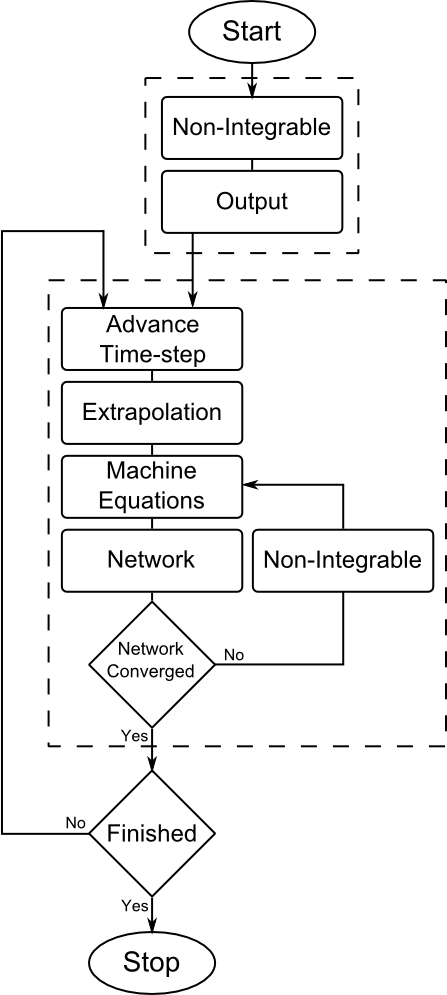
\includegraphics[scale=0.7]{simulatorflow.png}
      \caption{Dynamic Simulator Flow Diagram}
      \label{SimulatorFlow}
    \end{center}
  \end{figure}

The mathematical model is broken down in a number of ways to speed up the running of the simulation program:

\begin{itemize}
  \item The simulation time is broken down into discreet steps, normally of the order of 10ms. The time step can be varied such that during a fault a low value is used for accuracy while a large one is used to increase simulation speed.
  \item Each generators' dynamics are calculated separately from the others; this is then put into a load-flow to determine the voltages on the transmission system.
  \item The system is reduced from three phase to direct \& quadrature using Park's transformation \cite{Park1929,Park1933}.
  \item Within each generator's calculation, the linear and non-linear elements of the equations are solved separately. This allows the use of well established and fast methods for solving linear equations \cite{Brenan1987}.
\end{itemize}

The choice of algorithm for solving the linear part of the generator's equations is an important one. An incorrect algorithm will produce erroneous results, often without indication that they are wrong or it may simply take an inordinate amount of time to solve. The problem of producing erroneous results is exacerbated by the fact that the controllers in power systems often contain both small and large constants, which causes many methods for solving the equations to become unstable, regardless of whether the system you are simulating is unstable or not.

Systems that have both small and large constants are known as \emph{stiff systems}. Unfortunately the class of algorithms that provides the best results in terms of accuracy/time falls foul to this problem, having to use a very small time-step to overcome it. The small time-step means that more steps are needed to simulate the same amount of time, hence the simulation takes longer removing the previous advantage. One way to overcome this is to modify the equations by removing the small time-constants. However this is not a simple task. Wheatley \cite{Gerald2003} and Ascher \cite{Ascher1998} provide good comparisons of the different types of algorithm.

For transient stability modelling programs, such as the one being considered, the best algorithm is a trapezoidal integration algorithm, it is \emph{a-stable}, meaning it responds well to stiff systems. By repeatedly feeding the answer back in to the algorithm an estimate for the error can be obtained and used to alter the step-size or iterate to improve the answer.

There are different ways of mathematically describing a synchronous machine, and within that there are different levels of detail that can be considered. Milano \cite{Milano} gives a comparison of the different levels of detail for the \emph{voltage behind sub-transient method}; Dandeno \cite{IEEE2003} gives a comparison of the more popular \emph{flux-linkage} models. Both methods can work but to ensure correct results are obtained, a suitable level of detail within the models must be used.

\subsection{Numerical Integration}

A good numerical integrator is key to having a realistic simulator. In general a numerical integrator takes a set of equations describing a system, along with an initial condition, and calculates the state of the system at any point in time. In power systems the numerical integrator is used to find the solution to the linear components of the ODE.

The general form is where the integral ($\dot{x}_n$) can be calculated from the system state (${x}_n$) and the inputs ($u_n$) for any value of time Eqn \ref{eqn-system-states}. It also requires that the initial system states and inputs are known Eqn \ref{eqn-integration-initial}. The outputs ($y_n$) are simply a function of the states at that time: the inputs are a function of both states and outputs.

The objective is to be able to accurately predict the outputs at any given time given only this information \cite{Chang2006}. Sometimes the input changes based upon external factors but this does not change the calculation.

\begin{eqnarray}
\dot{x}_n = f( x_n, u_n ) \label{eqn-system-states}\\
y_n = g(x_n) \label{eqn-integration-output} \\
u_n = h(x_n, y_n) \label{eqn-integration-input} \\
x(0) = x_0, u(0) = u_0 \label{eqn-integration-initial}
\end{eqnarray}

\subsubsection{Euler's Method}

The most basic form of numerical integration uses a linear extrapolation from the current point using the slope known from Eqn \ref{eqn-system-states} to provide a rather crude estimate for the next system state. This only uses the known values of states, input and the time step duration: $h$ (i.e.\ the amount of time between two time steps) \cite{Lengyel2003}.

\begin{equation}
x_{n+1} \approx x_{n} + \left[ f( x_n, u_n ) \right] \label{eqn-euler}
\end{equation}

The error in each iteration is proportional to the square of the time step duration $h$. This is known as the \emph{local error}. Over a number of iterations the error is proportional to the time step duration and is known as the \emph{global error} \cite{Gerald2003}.

\begin{eqnarray}
localerror \propto O(h^2) \label{eqn-localerror}\\
globalerror \propto O(h) \label{eqn-globalerror}
\end{eqnarray}

\subsubsection{Heun's Method}

We know that Euler's method will always underestimate the correct value for lines whose slope is positive over the time-step in question. We can use the approximation for the system's states, $x_{n+1}'$, can be used to make another estimate, this time using the derivative from the new value. This will be an overestimate and hence by averaging we get a closer approximation to the real value.

\begin{eqnarray}
x_{n+1} = x_{n} + \frac{k_1 + k_2 }{2}  \label{eqn-heun} \\
k_1 = h \times f( x_n, u_n )  \label{eqn-heun-k1}\\
k_2 = h \times f\left( x_n + h, u_n + k_1 \right) \label{eqn-heun-k2}
\end{eqnarray}

\subsubsection{Runge Kutta}

This method takes the idea in the previous section further and makes multiple predictions and averages them together. The most common of these is RK4. It uses four weighted predictions using the derivative at each and the middle of the time-step.

\begin{eqnarray}
x_{n+1} = x_{n} + \frac{h}{6} \left( k_1 + 2 k_2 + 2 k_3 + k_4 \right)  \label{eqn-rk4} \\
k_1 = f\left( x_n, u_n  \right)\\
k_2 = f\left( x_n + \frac{h}{2}, u_n + \frac{h}{2} k_1 \right)\\
k_3 = f\left( x_n + \frac{h}{2}, u_n + \frac{h}{2} k_2 \right)\\
k_4 = f\left( x_n + h, u_n + h k_3 \right)
\end{eqnarray}

\subsubsection{Multi-step Methods}

The last three methods are all single step, that is, they all only use the current state to work out the next one. A more accurate estimate can be made for continuous curves if previously calculated steps are used. This will only work on systems that have the first few time steps specified, though these could be worked out using other methods. Other method include using higher order integrals of the system states. A summary of numerical methods for ODEs is given in Table \ref{tbl_numericalmethods}.

\begin{sidewaystable}[!p]
\caption{Comparison of Numerical Methods for ODEs}
\begin{center}
\begin{tabular}{|l|c|c|c|c|p{2cm}|l|}
\hline
\textbf{Method} & \textbf{Type} & \textbf{Local Error} & \textbf{Global Error} & \textbf{Stability} & \textbf{Variable step-size} & \textbf{Ref.} \\ \hline
Euler                     & single-step & $O(h^2)$ & $O(h)$   & good & good & Lengyel p.448  \\ \hline
Improved Euler            & single-step & $O(h^3)$ & $O(h^2)$ & good & good & Lengyel p.448  \\ \hline
Modified Euler            & single-step & $O(h^3)$ & $O(h^2)$ & good & good & Wheatley p.303 \\ \hline
Taylor Series             & multi-step  &          &          &      &      & Wheatley p.301 \\ \hline
Runge-Kutta 4  & multi-step  & $O(h^5)$ & $O(h^4)$ & good & good & Wheatley p.306 \\ \hline
Milne                     & multi-step  & $O(h^5)$ & $O(h^4)$ & poor & poor & Wheatley p.314 \\ \hline
Adams-Moulton             & multi-step  & $O(h^5)$ & $O(h^4)$ & good & poor & Wheatley p.318 \\ \hline
\end{tabular}
\end{center}
\label{tbl_numericalmethods}
\end{sidewaystable}


\subsubsection{Stability}

Although RK4 or multi-step methods provide great advantages in terms of speed and accuracy, they only useful if the solution is stable. This has nothing to do with the stability of the power system that is being modelled. Very stiff systems require very small time steps to give a correct answer, this cancels out any advantage gained by the superior method.

For any explicit integration method to be stable its time-step must satisfy the following relationship (where $\lambda$ is the largest eigenvalue and $\tau$ is the smallest time constant):

\begin{eqnarray}
h < \frac{2}{|\lambda|} \\
h < 2\tau
\end{eqnarray}

Certain integration methods are A-stable meaning they do not depend on the size of the time step. Linear implicit Euler (backward Euler) and \emph{trapezoidal integration} both have this property. Small time constants are simply not visible in the output rather than making the system unstable. As stated before the trapezoidal integration is the best method for such problems owing to its stability.

\subsubsection{Linear and Pseudo-Linear Systems}

Linear systems allow simplifications to increase the speed of calculation. Although power systems are highly non-linear they can be rewritten so that the non-linear components form algebraic equations giving new inputs to the system. In this way the advantage of linear systems can be utilised while only sacrificing a higher iteration number on highly non-linear parts.

\begin{eqnarray}
\underline{\dot{x}_{n}} = [A]\underline{x_n} + [B]\underline{u_n} \label{eqn-linear-state} \\
\underline{\dot{y}_{n}} = [C]\underline{x_n} \label{eqn-linear-output}
\end{eqnarray}

By substituting the above equations into the trapezoidal method a simplified form can be obtained that depends only on three constant matrices. To assist the costly matrix inversion the decomposition of one matrix into lower and upper triangular form can be performed. This \emph{LU decomposition}, as it is known, preconditions the calculated matrices. As these matrices stay constant in a power system a huge time saving can be achieved. The process of LU decomposition can be improved by pivoting. This changes the order of rows in the matrix to either reduce the error or keep the matrix as sparse as possible.

This is shown in Eqn \ref{eqn-trapezoidal}.

\begin{eqnarray}
x_{n+1} \approx x_{n} + \frac{h}{2} \left[ f( x_n, u_n ) +  f( x_{n+1}, u_{n+1} ) \right] \label{eqn-trapezoidal}\\
x_{n+1} \approx x_{n} [M] + [N] \left( u_n + u_{n+1} ) \right) \label{eqn-trapezoidal-linear}\\
M = \left( \mathbb{I} + \frac{h[A]}{2} \right) \left( \mathbb{I} - \frac{h[A]}{2} \right)^{-1}\\
N = \left(\frac{h[B]}{2} \right) \left( \mathbb{I} - \frac{h[A]}{2} \right)^{-1}
\end{eqnarray}

A further advantage of the trapezoidal method is that it is possible to iterate to improve the accuracy of the solution.

\begin{eqnarray}
(L.U)^{-1} x_{n+1} \approx x_{n} \left( \mathbb{I} + \frac{h[A]}{2} \right)
\end{eqnarray}

\subsection{Optimising Run-time Speed}

In addition to the method described above there are many less frequently used techniques available to increase the execution speed of dynamic simulations.

Power systems will give rise to \emph{sparse matrices}, that is most of the matrix will be filled with zeros. This can be exploited so that only the non zero sections of the matrices get calculated. Unfortunately other techniques can change the sparsity of the matrices giving the technique less impact. The matrices can be \emph{partitioned} so that larger areas are sparse or even so that different computing cores can calculate the result in parallel. There are many format for sparse matrices. After comparing a number of them (dense, linked list, CSR, CSC, coordinate format \cite{Saad1992} the vector of linked lists used in PSSENG was deemed to be best owing to the speed of both calculation and initialisation.

The reordering required for partitioning has a tendency to make one area of the matrix dense removing some of the aforementioned advantage. Chan \cite{Chan1992} worked extensively on matrix partitioning for an old version of PSSENG.

Rather than try to execute parts of the matrices in parallel a simpler method is to separate the execution by generator. As the simulator already separates generators for calculation and as they already have a low input and output they are ideal for \emph{parallel execution}. Managing the threads of execution would be difficult to do at the required speed but as multi-core chips are increasingly common it could provide significant advantages.

If the generators ODE calculations are being passed to another computation unit it would be worthwhile finding the best type of chip to use. Obviously the calculations will work on a general purpose CPU but the type of calculations involved mean that fast floating point arithmetic is advantageous. \emph{SIMD} is an extension to x86 instruction sets in most common computers. It is made specifically for pipelining floating point arithmetic for quick solutions.

Even more specialised is the GPU, or graphics card, is made for computer games. It excels at just the task required for power system simulation. Only recently have developers been able to use graphics cards for general purpose calculations (this is known as \emph{GPGPU} \cite{Che2008}). This would require a major rethink due to the idiosyncrasies of the device but the advantage should be large.

As the majority of the ODE calculations are fixed throughout the life of the simulation a possibility if to use a \emph{FPGA} set for the specific system. This programmable computer is a halfway house between hardware and software and could be used to give huge speedups in execution at the expense of a large set-up time.

Another possible improvement proposed by Rod Dunn of the University of Bath is to somehow separate the network equations by taking into account the speed of light. As nothing can move faster than light a fault on one area of a network has zero impact on far away components in the next time step. This separation should mean that arbitrarily large systems could be simulated with only a linear slowdown rather than the current exponential cost.

Finally optimisations can be done at the top most level; the entire simulation. Edwards \cite{Edwards1995} trained an \emph{Artificial Neural Network} (ANN) to recognise systems that would become unstable using only the first second of a dynamic simulation. That system decided if the system was definitely stable, the rest had a full 30 seconds of dynamic simulation to see the actual result. This filtered out the need for a huge number of simulations to be run and gave time for a simple SCOPF based upon a Genetic Algorithm (GA) to be run.

If many simulations need to be run on the same basic system then the problem is trivially parallelizable. Each simulation can be added to a queue to tasks. When a computer is free it simply grabs the next task off the queue. If there is a change that the exact system state will be asked to simulate repeatedly the result can be saved in a database rather than calculated again. This is called \emph{memoization}.

As with any optimisation careful profiling is necessary to determine if the proposed changes are worth the effort. At the rate computing power is increasing these methods, while advantageous, may fall short of the more pragmatic method of simply buying faster computers as they become available.


% ------------------------------------------------------------------ %
\section{Load-Flow}
% ------------------------------------------------------------------ %

\subsection{Load-Flow (Power-Flow)}

\begin{myquote}[\cite{Arrillaga1990}]The object of load-flow calculations is to determine the steady-state operating characteristics of the power generation/transmission system for a given set of busbar loads\dots The solution is expected to provide information of voltage magnitudes and angles, active and reactive power flows in the individual transmission units, losses and the reactive power generated or absorbed at voltage-controlled busbars\dots constraints make the problem non-linear and the numerical solution must therefore be iterative in nature.\end{myquote}

A load-flow is one of the most common forms of simulation owing to its simplicity and speed. To perform a load-flow we require knowledge of certain parameters on each busbar. There are three types of busbar depending on the components attached:

\begin{enumerate}
\item $PV$ - Voltage controlled busbar - Generator. Assumes P \& V held constant by power electronics.
\item $PQ$ - Von-voltage controlled busbar - Load. Assumes that P \& Q is not affected by small voltage changes.
\item $V\theta$ - Slack (swing) busbar. Corresponds to the one busbar that does frequency control.
\end{enumerate}

The $PV$ busbar represents a generator where we assume governor action holds the real power $P$ at a given value, hence it is specified and an AVR fixes the voltage in the same way. A $PQ$ is used for busbars without control from an AVR. These are mainly load centres without an accompanying generator, hence the complex power is known. It is assumed that the power will not be affected by small changes in voltage, a reasonable simplifying assumption in most instances.

One busbar is needed to take up the slack as the load-flow requires matched generator-demand balance and the line losses are unknown. This slack busbar has its voltage fully specified in both phase and magnitude. In most instances a phase balanced operation is assumed hence only one phase is modelled but it is possible to have a three-phase load-flow \cite{Arrillaga2001}.

Initial conditions are supplied to start the iterative equation assuming that the phase is zero and voltage is one for busbars where it is not known. The iteration continues until the mismatch between power and/or voltage is below a certain threshold.

A power-flow calculates complex power flow and losses on each power line as well as the following data for every busbar on the system:

\begin{enumerate}
\item $P$ -- Real (active) power
\item $Q$ -- Reactive (quadrature) power
\item $V$ -- Voltage magnitude
\item $\theta$ -- Voltage phase angle
\end{enumerate}

A load-flow is an invaluable tool but it has its limitations. Most of these come from its inability to simulate dynamics which results in  many stability effects being masked. It also has limits on its ability to accurately show the steady state effect of large disturbances.

A load-flow can be used in conjunction with a dynamic simulation to partly overcome these limitations . A dynamic simulation can determine a set of load-flow conditions that cause problematic transient phenomena. These conditions form \emph{constraints} that can be used with a load-flow to detect possible stability issues that it normally would not be capable of detecting.

A dynamic simulation and a real system will respond to a line outage in a complex way, whereas a load-flow can only compensate for the change by either changing the reactive power profile or changing the power of the slack bus. Because of this, a poorly designed load-flow simulation can become more a test of the capabilities of a slack busbar rather than the system as a whole.

Every generator will experience a slight change in power following a line fault on a real system. This relationship is non-linear but depends on network topology, prime mover inertia and generator droop characteristics.

A distributed slack busbar compensates for this shortcoming in the load-flow by having more than one slack bus. At its logical extreme, if every busbar acts like a slack busbar the load-flow will behave more like a dynamic simulation. It obviously will not be able to simulate dynamics but it is more likely to end up at a similar steady state solution.

This requires an equation stating how to split power between the slack busbars. This basically is a simplified simulation of inertia, control electronics and droop characteristics. The simplest possible way to achieve this is to assign the mismatched power to be made up by the slack generators according to their current power output. Pseudo-code for this mismatch fixing is given in Appendix~\ref{lbl_sec_code}.

Work was done to modify CPF to allow a load-flow to more accurately deal with faulted systems by using this special form of distributed slack bus.

\subsection{Optimal Power Flow (OPF)}

Owing to their rapid simulation speed, load-flow programs can be embedded inside optimisation programs. There is a variety of things that can be optimised, as well as a variety of techniques for the optimisation \cite{Zhang2007}. PSAT includes an optimal power flow (OPF) program which selects the lowest cost generation that has a load-flow solution without overloads.

This kind of OPF can be seen as an incredibly simplified simulated SO in that one of the roles of the SO is to run the cheapest generation available. The SO's other main operational role is to ensure security; there has been work done on creating automatic security constrained OPF programs but there is still much to be done in that field.

% ------------------------------------------------------------------ %
\section{Modelling Wind Power}\label{lbl_sec_model_wind}
% ------------------------------------------------------------------ %

Wind turbine output is unscheduleable it therefore needs to be predicted unlike conventional generation. Modelling wind farm output is a complex task. Not only do the electromechanics of the machinery need to be considered but so to does the weather.

There are different methods required, depending on the data available and the type of task. If, as in the case of this thesis, an artificial system is used then there is not going to be any real data. It is therefore a task of matching a realistic set of data onto the system.

In a real system there is likely to be some form of historic wind speed database. These speeds can be taken at face value but it is unlikely that there will be a large data-set available at the wind turbine sites themselves. Most data is from weather stations. The task then becomes a case of finding how different the turbine site is to the nearest weather station. This task is known as MCP analysis (Measure Correlate Predict) \cite{Thoegersen2007, Rogers2005}.

Synthetic data may be preferable \cite{Sturt2009} even if a real system is used as the basis for study. The main advantage is that synthetic data does not suffer from a limited number of data points to draw upon -- more samples can be taken at will.

\subsection{Wind Speeds}
The wind speeds are chaotic and dependent on a number of factors. They are both spatially and temporally correlated. This spatial correlation is not just a function of distance but is effect by terrain including valleys, vegetation and buildings. Work by the University of Bath separated the UK into 20 zones, further split by terrain type (lowland, highland, coastal, offshore) to ensure a more accurate model \cite{UniversityofBath2006}.

The time correlation has many periodic cycles, most notably diurnal and seasonal effects as well as short term gusting. Weather fronts will show a change of wind speed moving across a region over a period of time. There is even a correlation with demand level through temperature; a low temperature will affect wind speed as well as causing an increase in demand. This means wind speed prediction is highly complex; luckily there are synthetic models as well as historic data available.

\subsection{Wind Farms and Turbines}

Aside from the wind speed the design of individual turbines as well as the wind farm needs to be accounted for.

The altitude that wind speed is measured at a weather station is often 10m. This is well below the hub height of a wind turbine and hence the speed needs to be altered to reflect this. The term for the way wind speed changes at altitude is wind sheer. This is often a significant effect especially with the hub height of newer turbines reaching over 100m.

The layout of a wind farm will cause two significant effects. One is that there will be wake losses caused by having many wind turbines in one area. Careful planning can reduce this but in \cite{Pudaruth2009} wake losses account for an 8\% reduction. There will also be the positive effect of spatial smoothing. A wind farm will have the effects of gusting averaged out across each turbine leading to less dramatic changes in power when compared to single turbines. This averaging effect also takes place across the country but this effect should automatically come out of the wind speed model.

Early research by the author involved looking into so called `3p` effects. This included the drop in power as each of the three blades passed the tower. On its own the magnitude would not be great but if blades were to synchronise, either from electromechanical effects or wind movements, the effect could be significant. A literature review, shown in the next section, indicated that this effect was negligible and that wind farms could be modelled as a single turbine for system-wide studies.

There are standard equations \cite{Ackermann2005} for converting a wind speed into a generator output power for certain types of turbine and blades. There is four parts to this curve Fig \ref{WindPowerCurve}. The first is where the wind speed is insufficient to cause any generated power at all. Next the power ramps up almost linearly to a maximum before reaching a cut-off where the blades are forced to stop moving to prevent damage to the machinery.

\image{WindPowerCurve}{Wind Power Curve \cite{BWEA2005f}}{windpowercurve.png}

The cut-off region is of great interest as there is a large change in power for a very small change in wind speed. It is not hard to imagine a situation where all wind farms are running at full capacity allowing conventional generators to be switched off. If then wind speed was to increase across the country many wind farms could suddenly stop generating due to this safety cut-off. Because of this a larger amount of spinning reserve is required.

\subsection{Dynamics and Power Electronics}

There has been much work done in the area of wind power generation modelling. The Electrical Power Systems Group, Delft University of Technology, Netherlands provides great detail on dynamic modelling of wind turbines, especially the work by W. L. Kling, J.G. Slootweg, H. Polinder. The most relevant of their work is on initialisation of wind turbine models \cite{Slootweg2001}, and two papers on the modelling \cite{Slootweg2001a, Slootweg2001b} culminating in a “General Model for Representing Variable Speed Wind Turbines in Power System Dynamics Simulations” \cite{Slootweg2003a}.

Their work progresses in two directions.

\begin{enumerate}
\item In creating an aggregated model for wind farms \cite{Slootweg2003}, where it is found that their combined model accurately reflects the detailed model they had created before, even during fault conditions, confirmed by other studies \cite{Castro1996}.

\item They look at the stability effects of distributed generation \cite{Reza2003, Reza2004, Slootweg2002a, Voorden2001} and find that, due to the inability for induction generators to control reactive power, they are a destabilising influence on the network as a whole, whereas double fed induction generators (DFIG) are much more stable.
\end{enumerate}


This is reflected in work by other Institutes which say that normal induction generators can cause voltage sags \cite{Holdsworth2001}, which can lead to voltage collapse, and that double-fed induction generators are not only better than normal induction generators, they are better than synchronous machines due to their power electronics \cite{Usaola2001}. By having a generator that causes voltage collapse during faults they must be tripped. This adds to the severity of the fault \cite{Eriksen2005}. Luckily most recently installed generators are of the variable speed DFIG type.

Reactive compensation can overcome the destabilising effect of fixed speed wind turbines as shown by Palsson et al. \cite{Palsson2002} but these are expensive components.

It is also possible that power storage devices, like flywheels, could average out fluctuations but this technology is not widely exploited and is expensive. Nick Jenkins at Electrical Energy and Power Systems, The University of Manchester, UK takes a higher level approach by looking at the stability aspects of large wind farms on the transmission network \cite{Jenkins1997}.

The paper by Thomas Ackerman et al., at Royal Institute of Technology, Sweden, covers many aspects of wind power security \cite{Eriksen2005}.

\begin{myquote}[\cite{Eriksen2005}]The TSO had been unable to assess the impact of wind generation on system stability due to the lack of suitable dynamic models.

With increasing wind capacity, the TSOs became concerned about the impact of high levels of wind generation on system stability. The integration of wind power has been hampered by the lack of suitable dynamic models for use in transient stability studies.\end{myquote}

Although they go on to say \inlinequote{Wind Turbines do not cause transient stability or any dynamic oscillation issues}, they do agree that scheduling can become problematic. \inlinequote{High wind power penetration levels require a rethinking of the power system operation method because wind power cannot be scheduled with the same certainty as conventional power plants.} In terms of variability the paper says, \inlinequote{large turbines with variable speed operations tend to absorb gusts} and short term fluctuations may become a problem when large off-shore farms are installed. Wind power reductions due to the cut-off can, in extreme situations lead to very large power deviations.

Finally, they state that increasing wind power penetration usually requires more frequent usage of long-term reserves, which would increase balancing market prices, and that wind output may have to be curtailed for stability reasons.


%Goran Strbac at the Electrical Energy Systems, Imperial Collage London, UK has looked extensively into the financial aspect of integrating wind generation.

\section{Chapter Summary}

There are different techniques for reasoning about a power system. This chapter compares different methods. Two in particular, load-flow and dynamic simulations, are explored in detail. This is due to the fact that simulation accuracy and speed are vitally important to the success of the proposed work. There was extensive work done to try and create a very fast dynamic power system simulator. This presented a few promising areas of future work. The chapter ends with a detailed look at the specifics of modelling wind farms.





% ================================================================== %
% ================================================================== %
% ================================================================== %









% ================================================================== %
\chapter{Security Assessment Schemes}\label{lbl_ch_SAS}
% ================================================================== %

This chapter introduces the problem of security assessment from the point of view of a system operator (SO). After detailing the problem it goes on to compare the traditional deterministic schemes with the less used probabilistic method.

\section{The Role of the System Operator (SO)}\label{lbl_sec_so}

The task in security control is to keep the system in the normal state. The normal state is defined as having all system variables within normal range with no overloads; that the system operates securely and is able to withstand a contingency without violating the constraints \cite{Kundur1994}. Security assessment is the analysis of data from security monitoring. The decentralisation of power markets has caused power systems to be driven closer to their operation limits, trading off security for cost. The optimal way to do this trade-off is by having the most accurate security assessment schemes available.

If a sub-optimal security assessment scheme is used it may lead to costly over-securing in certain conditions and dangerously low security in others. This will mean that higher safety margins must be put on poor security schemes which will lead to an unnecessarily high cost.

An accurate scheme should take into account both likelihood and consequence of every possible event. In fact a security assessment scheme should accurately represent the risk of running the system in the current state where risk is a function of both likelihood and consequence for every possible event \cite{Billinton1997}.

\begin{equation}
  \label{eqn_risk}
  R = \sum\limits_{i}^{} L (e_i) \times C(e_i)
\end{equation}

Where $R$ is Risk, $e$ is an event, $L$ is likelihood, and $C$ is consequence. A further definition of security \cite{Balu1992} gives further insight into the problem:

\begin{myquote}[\cite{Balu1992}]Security may be defined as the probability of the system's operating point remaining in a viable state, given the probabilities of changes in the system (contingencies) and its environment (weather, customer demands, etc.).\end{myquote}

A perfect system is infeasible in practise due to time constraints. In the UK, system operators have only one hour to perform final balancing actions between the FPN - the point when they are supplied with the final load/generator data, and the point of delivery. Though the balancing market lasts only one hour, the system operator is likely to make predictions on generator bids beforehand for use in preliminary calculations. Power system security is all about coping with likely changes. Kirschen \cite{Kirschen2002} provides a good overview to some of the challenges involved.

Security cannot easily be defined in absolute terms; there are many trade-offs to be made. The goal is to achieve an acceptable level of security, at the least cost. To deal with the massive complexity involved in this calculation many simplifying assumptions are made and the use of computer simulations are invaluable.

\section{Security Assessment Schemes (SAS)}

The term Security Assessment Scheme (SAS) means a set of rules that are required for a power system to be called secure. For instance N-1 is a SAS which states that a system can be called N-1 secure if, and only if, any single component outage still leaves the system in an acceptable state. Obviously for this scheme to be used in practise the set of components to be considered needs to be more accurately defined as well as the term `acceptable` in this context. SAS are used to ensure a system remains reasonably secure. If the system fails the SAS then further operator action must be taken to ensure it passes. This necessitates simulation to verify the contingencies that are considered.

A SAS in the context of this work does not match wholly with reality. In the UK the SO, National Grid, has a team of engineers creating predictions, contingencies and constraints months in advance of delivery. The predictions are based upon expert knowledge aided by scores of specialist programs and simulations. These are handed down to other teams to refine and update based upon better predictions. These form a set of likely events which are tuned, not only to the specific system, but to the weather, time of day, and even the schedule of TV. Finally, when the FPN (final physical notification) is received, only minor tweaks \emph{should} be needed to be made. Then, as power is delivered, automatic actions as well as constant manual tuning keep the system in check.

This thesis uses a more simplified idea of security assessment. It assumes that one program is given the task of assessing whether the state the power system is in is acceptable. It is therefore the purpose of a security assessment scheme to return either a pass or fail for a system in a given state. The system operator then makes balancing actions which change the system state until it has passed the SAS.

If the SAS reports too many operating conditions as passes then costly emergency operator action will be regularly required. If it reports too little passes then the system is being needlessly over-secured at additional cost. Therefore there is an optimal level of security for the system, henceforth known as the security threshold. There is a direct trade-off between security and cost, which must be managed.

\section{Designing Goals of a SAS}\label{lbl_sec_design_goals}

There are five criteria that a SAS should be measured against. It should be:

\begin{itemize}
  \item Economic,
  \item Secure,
  \item Fast,
  \item Verifiable, and
  \item Fair.
\end{itemize}

The role in designing a SAS is not only to pick the best level of security for the system but also to make sure the SAS accurately represents the security level. The problem arises because we cannot accurately determine the security of a power system in a given state. The assumptions made in designing a SAS may lead to certain conditions being over-secured and others under-secured. The more accurately the SAS can be designed, the lower the margin of error and the greater the financial savings.

In this context we use the definition of security given in \cite{Kundur2004} - that security is the ability of a power system to remain stable and within operational limits following any likely disturbance. In this way security is a function of both the current state of the system and any changes that occur during delivery. It is for this reason that weather can effect the security of all power systems, even ones without renewable generation.

Given this definition it not easy to quantify the security not only due to the number of unknowns but also due to its multi-faceted nature. For the purpose of this discussion let us assume the security level of a power system in a given state can be calculated as a number. Further, let us assume that we have a large number of likely system states. A perfect security assessment scheme would report a pass to all systems that have a security level above the security threshold and a fail to all those below.

\image{perfectSAS}{Example of a Perfect SAS}{perfectsas.png}

This can be visualised as follows: Assume that the security level of a power system in a given state can be represented by a number between 0 and 100, where the higher number is more secure. Further, let us assume that the security threshold is 50, i.e.\ we want a SAS that reports a pass for all systems with a security higher than 50. This is shown in Fig \ref{perfectSAS}.


Fig \ref{SAScomparison} shows a number of different theoretical SAS marked against the same set of system operating conditions. We can see that \ref{SAScomparison}-a is perfectly accurate and precise. It only ever reports a pass to those over 50. This is impossible to achieve in practise due to time constraints.

\ref{SAScomparison}-b is equally precise but the additional passes mean it has low accuracy and is under-secured.  If this was used as a real SAS we would expect emergency operator action to be regularly required.

\ref{SAScomparison}-c is again precise with low-accuracy but this time it is over-secure. The downside to this option is cost. As stated for \ref{SAScomparison}-a it is not possible to have a perfectly precise SAS; \ref{SAScomparison}-d shows a lower precision SAS with high accuracy. This is more like what would be expected from a real SAS.


  \begin{sidewaysfigure}[!p]
    \begin{center}
      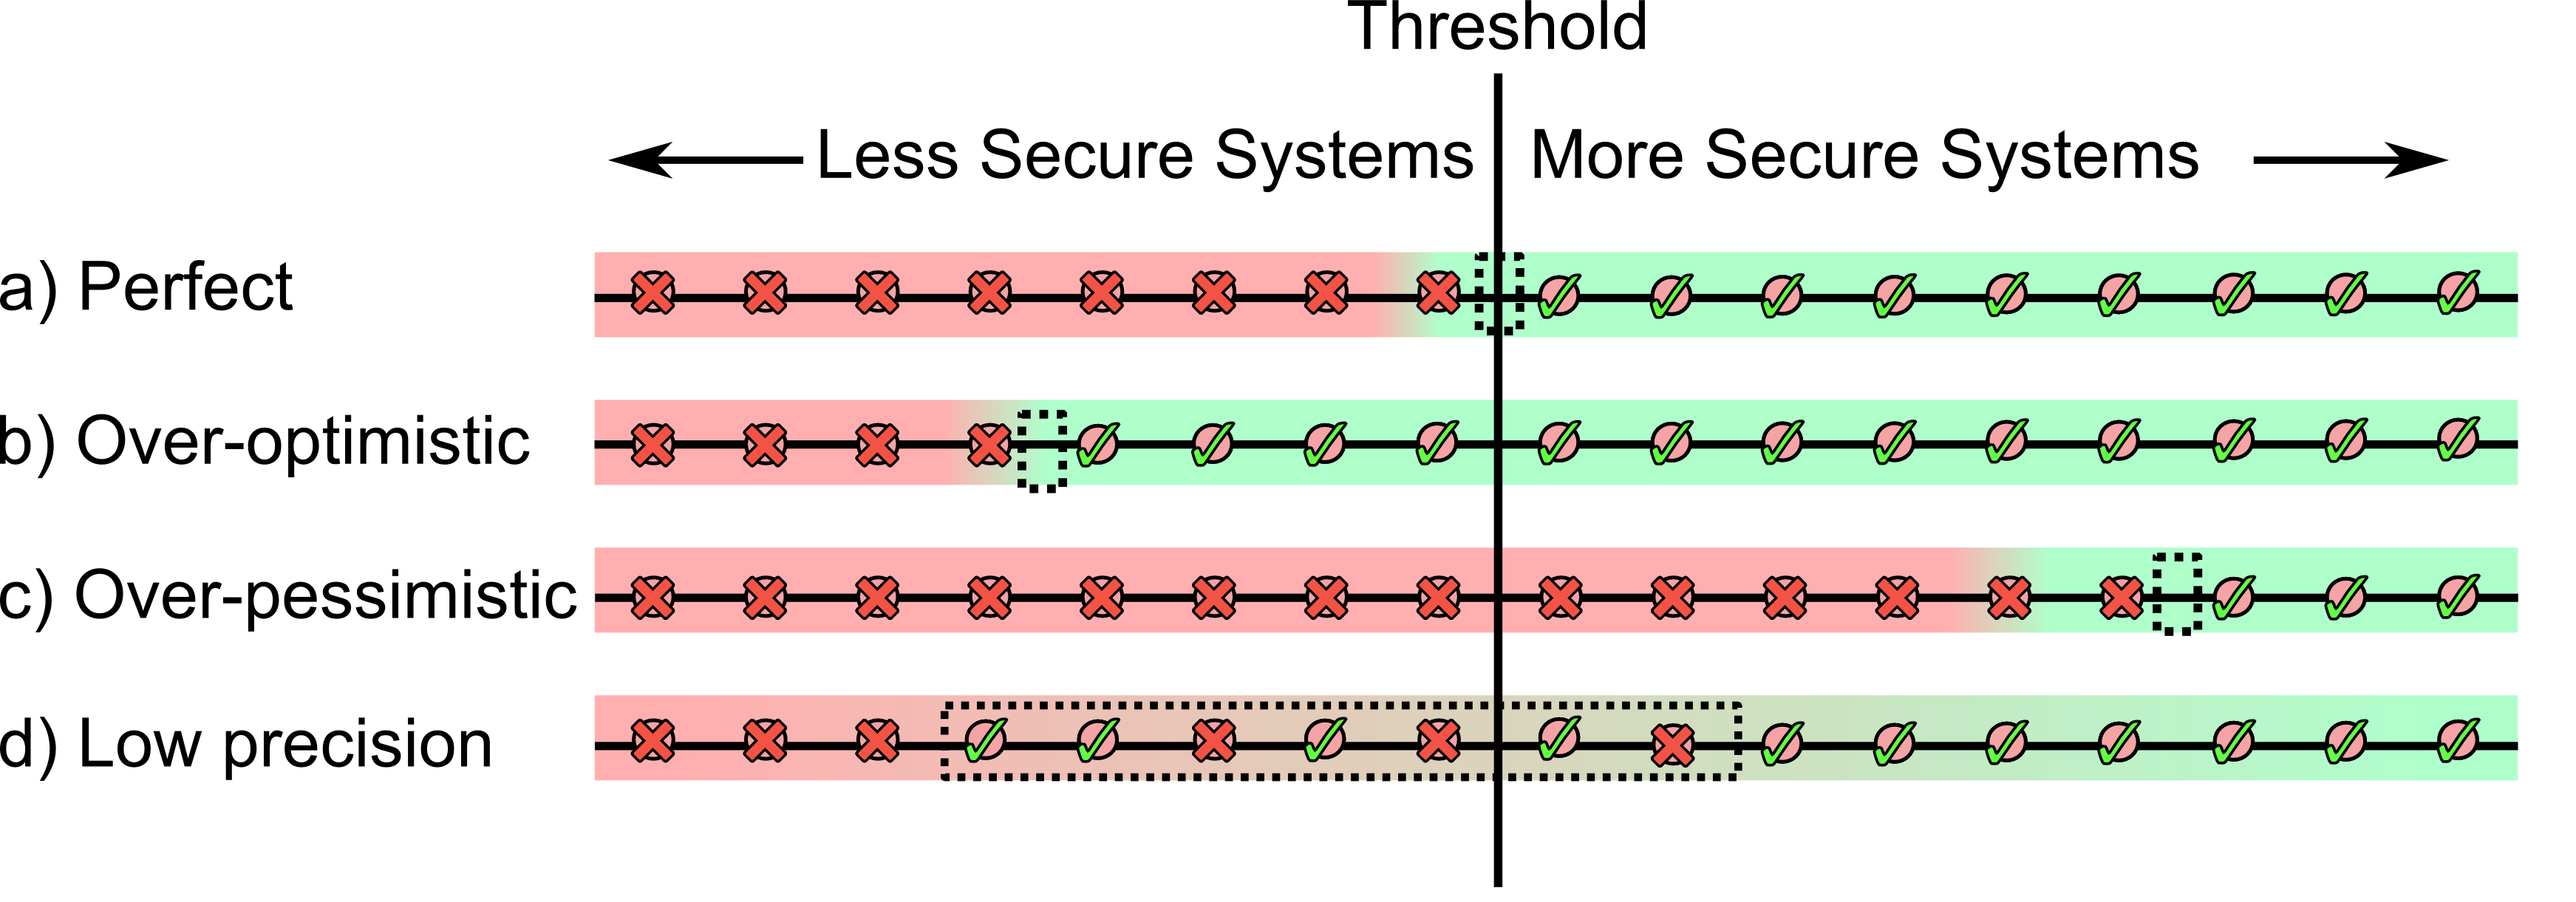
\includegraphics[scale=0.7]{sascomparison.png}
      \caption{Comparison of SAS}
      \label{SAScomparison}
    \end{center}
  \end{sidewaysfigure}



If we have a very low precision SAS then it would have to be altered to be over secure. The reason for this is that only a certain frequency of interruption will be accepted. To ensure that a low precision SAS will have this low frequency of interruption it must have a built-in safety margin. This safety margin is costly.

In addition to the precision and accuracy of the SAS, which give rise to cost and outage rate, there are other criteria that must be addressed. Firstly, the results must be verifiable; that is following an incident such as cascading outages or brown-outs it must be possible to determine who, if anyone, is at fault. The SO has a responsibility to maintain an acceptable reliability and if it had used an inadequate SAS or the SAS is not being used correctly then they should be held accountable. But as stated above there is an optimum level of security and therefore an optimal number of cascading outages, brown-outs and loss of load. If the SAS is deemed adequate and was followed correctly then a certain number of faults should be expected as part of the benefit of having cheaper electricity.

A further requirement is that it does not disadvantage any particular generator and ideally should allow for environmentally friendly operation by rarely curtailing renewables. It has been the case in the UK that wind generations have had to be curtailed for stability reasons.

This must all be able to be run fast enough for the SO to make an necessary modifications and rerun the SAS until the system is adequate.


\section{Deterministic Power System Security}

Traditionally, security assessment schemes manage this complexity by using a set of credible contingencies. These are meant to represent all likely events with a severe consequence -- they should be events with the largest product of likelihood and consequence. There has been significant work in determining which events to include \cite{Balu1992, McCalley1999, Donde2008}. These contingencies are often different for each half-hour delivery period and vary based upon weather and season.

The set of normal contingencies that are considered is given in \cite{Kundur1994}; a sub-set of this is known as \emph{N-1}. N-1 is a security assessment scheme that considers the failure of one component (line, generator or transformer) at a time. In other words, the simultaneous failure of two components is considered too unlikely to count. There have been various modifications to N-1, including the addition of correlated failures, such as the failure of two lines on a common right-of-way.

The UK SO does consider a sub-set of N-2 contingencies where two simultaneous failures are considered but not all possible double failures are checked. This traditional contingency screening has worked well for many years but with the paradigm shift in generation, that is coming in the form of local, unscheduleable generation, it is time to review this idea.

The problem with all such N-x methods (N-1, N-2, etc.) is that they treat likelihood in such a crude way; it assumes all contingencies to be equally likely.

Another disadvantage of any deterministic security assessment scheme is that it can lead to problems if something outside of the expected set happens.

In the UK, the simultaneous failure of two generators was considered non-credible; hence, after it occurred during 2008, emergency operator action was needed. This is far from the only incident of its kind. 2003 saw more than its fair share of major incidents with North America, Libya, London and Italy \cite{El-werfelli2008} all experiencing widespread black-outs.

The credible disturbances are no longer best represented by discrete events. The change in wind power over a one hour period is significant, spatially correlated and continuous. It is possible to treat wind power as a contingency by quantisation at a large resolution into a small number of likely states. In performing this method one must be careful to have enough possible wind states to accurately represent everything that could happen.

If wind farms continue to be built at the current rate wind power will become a major component of the UK's plant mix. Unless the market changes this is likely to disadvantage wind farms due to their uncertainty \cite{BWEA2005}. Some may say that their cost will accurately reflect their difficult of incorporating such uncertainty in a power system but there is no point in building wind turbines if they are not to be fully utilised.  Renewable power should be encouraged from an environmental point of view. However the technical challenges must be overcome. In reality the likelihood is that the wind resource as a whole will not fluctuate drastically, especially if turbines are distributed over a large geographical area. But the risk must be quantified and verifiable before new security assessment methods can be implemented.

\section{Probabilistic Power System Security}

Risk-based, probabilistic, security assessment uses probability much more directly. It is not a new idea, it has been used in other industries since the 1960's; and has been studied in power systems since the 1970's \cite{Patton1972}. But it is computationally expensive and often harder to produce a verifiable result. As the disadvantages of deterministic methods impacts financially, the focus has begun to turn towards probabilistic methods \cite{McCalley1999, Kirschen2002}. This is already happening as balancing market prices have been driven up by wind power \cite{BWEA2005}.

Sobajic et. al. \cite{Sobajic1989} provides a brief overview of four different approaches to the problem of stability assessment. The paper then discusses one such pattern recognition method after highlighting the works of Patton, Billinton, and Wu as contributing significantly to probabilistic methods.

After an extensive literature review, including the mention of Monte Carlo methods, McCalley \cite{McCalley1997} goes on to determine a set of deterministic rules based upon risk-based methods.

Monte Carlo methods are a type of algorithm used commonly in risk assessment where a system with uncertainty is repeatedly sampled. In this way Monte Carlo Methods lend themselves well to the task of probabilistic risk assessment. A comparison of different modifications to standard Monte Carlo Methods is given in \cite{Bell1999}, there a financial value is placed upon outages to give an absolute level of comparison.

For an up-to-date review of the work in risk-based security assessment see \cite{Kirschen2007}. It also provides a good conceptual representation which shows how risk-based security assessment will more accurately reflect the actual level of security. Xiao \cite{Xiao2007} shows graphically how traditional SCOPF can produce a more risky solution due to its fixed constraints.

By assigning a severity to each type of disturbance Ni \cite{Ni2003} created a system for aiding control room decisions based on risk.

\section{Limitations of N-1 Security}

The list of contingencies to be simulated has traditionally been where each line, transformer, and generator are individually taken out of service \cite{Kirschen2007}. This generates a set known as N-1, where N represents the number of system components; to be N-1 secure is to have a system which remains stable after any N-1 contingency occurs. The UK operates somewhere between N-1 and N-2 security (the set of all possible failures on any two components); that is, any single component fault and credible double fault should not cause the system to enter an emergency state.

In this way N-x security treats the probability of failure in a simplistic way; it assumes all contingencies to be equally likely. It fails to recognise that intermittent non-scheduleable generators have a quite inaccurate prediction of their output power \cite{Bathurst2002}. It also fails to take into account correlated failure caused by common right of way, common structure or extreme weather conditions.

Additionally, the set of credible disturbances is no longer discrete. This means the contingency analysis itself is losing some of its past merit. In the case of wind generation the output is stochastically variable, by treating it as a contingency you ignore the fact that the output can vary continuously between its rated capacity and zero power output. Using traditional security assessment will increasingly disadvantage renewable generation as penetration grows \cite{BWEA2006}. The treatment of variable load or supply under N-1 would be one of three cases:

\begin{enumerate}
  \item It is treated as an insignificant variation and hence taken at its expected value. This is how variation in load is currently treated.
  \item The worst case of possible values is used for testing against each contingency. For wind this would be either no output or maximum output.
  \item The variation is treated as a separate contingency, meaning it would not be tested in conjunction with other faults.
\end{enumerate}

To treat the curtailment of wind power as a separate contingency means that it will not be considered in conjunction with other faults in a N-1 security analysis, this will cause an over estimation of system security. Whereas, if it is treated as a unknown variable and hence put at its worst case, i.e.\ either full or no power generation, then wind will be the cause of an under estimation in system stability. For an individual generator there is only a 29\% chance that the output will remain within 5\% of what it currently is; but there is an almost negligible chance of it changing across its entire installed capacity. For this reason wind cannot be treated as an insignificant variation.

In reality there is a certain probability that the output will be at any particular value. This probability density function can be constructed from historic wind data. These have to be considered with each contingency. For instance the stability must be assessed while the wind is doing X with contingency Y.

\section{Chapter Summary}

This chapter sets out exactly what is required in a security assessment scheme. It then performs a thorough literature review of security assessment focusing on comparisons between deterministic and probabilistic methods. This leads to an analysis that forms the basis of the novel work presented in later chapters. The chapter finishes by detailing the problems faced by using deterministic N-1 security.


% ================================================================== %
% ================================================================== %
% ================================================================== %





% ================================================================== %
\chapter{Comparing Security Assessment Schemes}\label{sec_compsas}
% ================================================================== %

This chapter covers how security assessment schemes are assessed and compared then proceeds to detail the creation of a new method for comparing security assessment schemes. Finally, results are presented showing the novel method in action.

The work is based around a two stage Monte Carlo Sampler which uses a load-flow simulation of the IEEE-RTS Area 1. The first stage generates \emph{scenarios}, representing possible states the power system could be in. The second stage is used to create the probability that each of the scenarios from the first stage are acceptable. In this context acceptable means that no emergency operator action is required during the half-hour delivery period. This data is then tabulated to form an overall picture of how secure the system is in a number of cases. This can be useful in its own right but it can be further used to compare security assessment schemes as described below. The outline for this process is given in Fig \ref{figprograms}.


  \begin{sidewaysfigure}[!p]
    \begin{center}
      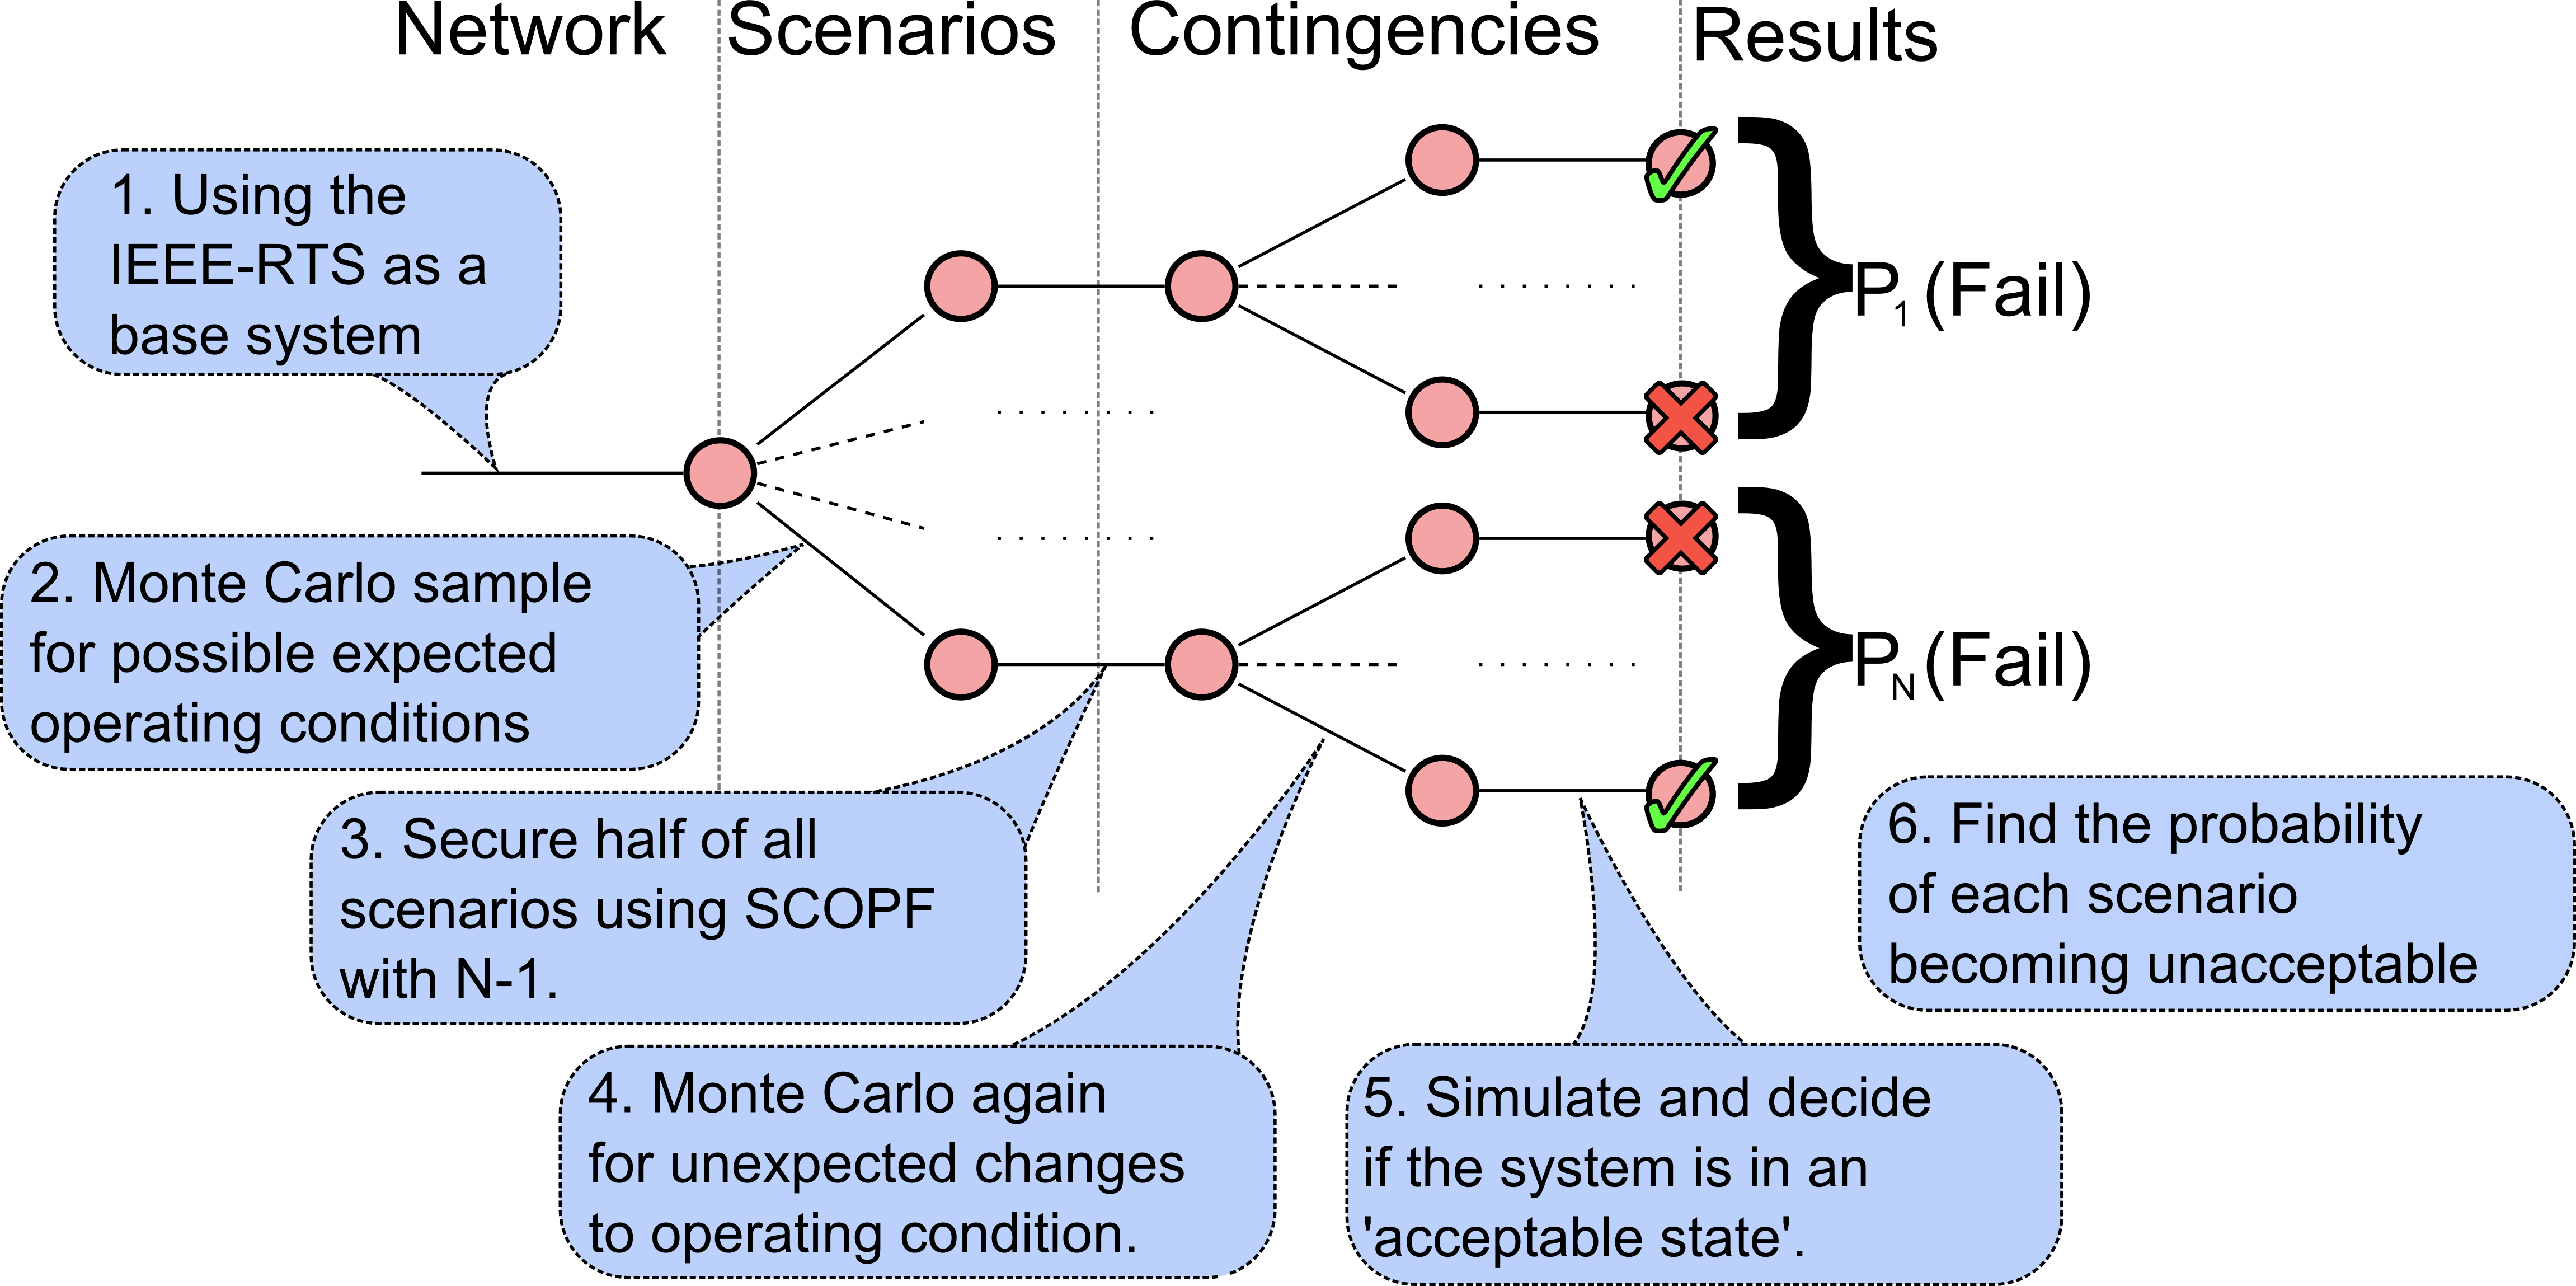
\includegraphics[scale=0.8]{overview.png}
      \caption{Structure of Comparison Program}
      \label{figprograms}
    \end{center}
  \end{sidewaysfigure}






% ------------------------------------------------------------------ %
\section{Method of Comparison}\label{lbl_sec_comparison}
% ------------------------------------------------------------------ %

Although there is significant work on different types of security assessment scheme and how well they perform there is relatively little work performing a direct comparison between two such schemes.

Lets say we have a SAS such as N-1. In other words the system is said to pass N-1 if the failure of any one component does not leave the system in an unacceptable state. We can test N-1 against each of our many operating conditions and see if it passes or fails. This can be shown graphically as in Img~\ref{SAScomparison} above. We can take a number of factors from the results that this gives us. Firstly we known for this specific set of operating conditions how many times our SAS under test differs from the perfect SAS described above. Obviously we want a low number of cases where they are in error.

We can also see whether the operating conditions that were in disagreement were false-positives or false-negatives. A false positive means a pass on the left of the security threshold; this is a system more likely to cause a problem than has been planned for. It is an under secure system. A false negative, a fail to the right of the threshold, represents an over secure system. It is likely that a SO would consider a false positive (under-secure) worse than a false negative (over-secure).

By looking at the specific operating conditions that were in disagreement it may be possible to determine whether the SAS is lacking in some respects. It may, for instance, misrepresent only systems where the wind variability is high.

We can also gather information by looking at the difference between each of the points in disagreement and the threshold. This gives an indication of how badly the SAS is when errors do occur. If a very insecure system, say with a security level of 10 is reported as a failure by a SAS then this is a larger problem than one with a security level of 49. A system with a security level of 10 is very likely to have some problem during its operation. This is by definition. If we allow such a system to run in that state then we are open to the financial cost of whatever stability or limits violation will occur. We can sum up the difference between each operating condition in disagreement and the threshold to come up with a value for the severity of error in the SAS. It should be noted that this number is not meant to represent anything in reality but is simply an indication of how well the SAS is for those operating conditions tested on that specific system. It can however be compared to another SAS run over the same operating conditions on the same system, to see which is best.

\section{Monte Carlo Sampling}\label{lbl_sec_mcs}

Monte Carlo Sampling (MCS) is simply the term given to the random sampling of events by their probability. If enough samples are taken properties of the underline system can be understood. The alternative to MCS is analytical techniques these, rather then performing sampling, use the probability data itself to gain knowledge of the underlining system.

For instance if we want to know the probability of a fair coin landing on heads three times in a row we can either use the analytical technique which simply gives $0.5^3 = 0.125$ or we can perform MCS. For this a computer program would be set up so that a pseudo-random number generator (PRNG) produces uniformly distributed numbers between 0 and 1. If the random number is above 0.5 the result is a head, otherwise it is a tail. After performing many samples we can see how many had three heads in a row as a percentage of the total. This should approximately match the analytical value but as MCS is a random approximation it cannot be expected to get the result perfectly.

Obviously in this example the analytical technique is far simpler but in other applications, such as the one needed for this thesis, analytical techniques become more complicated than MCS. To cope with that complexity large simplifications must be made in the analytical techniques meaning that for complex problems MCS is preferable.

The only caveat for creating a good MCS program is to ensure that the PRNG is suitable. Many programming languages come with random number functions by default but often these are not suitable for MCS. Pudaruth \cite{Pudaruth2009} provides a good comparison of random number generators. He concluded that the Mersenne Twister is the best suited, having both fast execution speed and a colossal period. Further discussion on the generation of random numbers is covered in the classic computer science monograph The Art of Computer Programming \cite{Knuth1998}.

The work detailed later was created in Python which used the Mersenne Twister as its default PRNG:

\begin{myquote}[\cite{Python}]Almost all module functions depend on the basic function random(), which generates a random float uniformly in the semi-open range [0.0,~1.0). Python uses the Mersenne Twister as the core generator. It produces 53-bit precision floats and has a period of $2^{19937}-1$. The underlying implementation in C is both fast and thread-safe. The Mersenne Twister is one of the most extensively tested random number generators in existence. However, being completely deterministic, it is not suitable for all purposes, and is completely unsuitable for cryptographic purposes.\end{myquote}

There are two ways MCS can be used: sequential and random. Sequential sampling builds up a time history of events through sampling whereas random MCS takes independent samples with no time history. Both are equally accurate and must be chosen on their other merits. Due to its faster execution random MCS should be chosen unless a time history is required.

One case where sequential MCS is preferable, as highlighted in \cite{Billinton1996}, is the modelling of pumped hydro storage. The current stored water depends on the power generated in previous samples, hence is best modelled sequentially. This is true of any component with storage that lasts longer than the period of one sample. It may be possible to model the level of storage as a partly random parameter if sequential analysis had shown that it would be accurate enough. In that way even pumped hydro storage could be modelled by random MCS but the extra work, as well as loss of accuracy, means that is rarely done.

Another case where sequential sampling may be required is if the failure rate of a component depends on when it last failed. This is best modelled sequentially because of the time history but if analysis has shown it would be acceptable this could be converted for use in random MCS.

Random sampling is used for the work in this thesis as there are no components that have a significant time dependency.

\section{Modelling of Monte Carlo Parameters}

For a Monte Carlo Sampling program to work well it must have good input probabilities. This sections details some of the possible factors that could be taken into account when creating a MCS program for this purpose.

\subsection{Wind Power Forecasting}

This has been discussed previously in Section \ref{lbl_sec_model_wind}. The simplest method of adding wind into the IEEE-RTS is to fit an existing historic model, such as the UK data available from the MET Office, over the geographic topology given in \cite{Grigg1999}. A more accurate method would be to create a synthetic model which would allow many more samples to be taken without repeating.

\subsection{Wind Forecast Error}

If historic data was used for forecast, then finding the forecast error is simply a case of taking the difference between two successive samples. Persistence forecasting is the name given to the assumption that the wind will stay the same over the time period. At such a short timescale, persistence forecasting is not far behind numerical weather prediction (NWP) methods and is far simpler.

If synthetic wind data was used, then a method such as the one proposed in \cite{Bathurst2002} could be used. This creates a statistical model of the change in wind speed. The report `Operating in 2020' by National Grid \cite{Grid2009} shows that there is a correlation between time of day and wind forecast error, though this may be more due to the difference in load level at those times.

\subsection{Load Forecasting \& Load Forecast Error}

At its minimum the load forecast should have diurnal, weekly, and seasonal cycles. The model in the IEEE-RTS covers all these. There are likely to be much more accurate models available but the supplied data is suitable for the studies required.

\subsection{Component Outages, Maintenance and Correlated Failures}

Component outages can be modelling in many ways, the simplest of which is based around the mean-time-to-fail (MTTF) and mean-time-to-restore (MTTR). Often a two state model is made where separate MTTF and MTTR values are given for good and adverse weather. Line faults are more common during adverse weather hence using separate values is more realistic.

There is also correlated failures to consider. If a single external event can cause the loss of more than one component then this should be considered. One example of this is where two separate transmission lines are located on the same physical tower. Damage to one line can cause damage to the other.

Maintenance is a more complex issue. A generator will only be scheduled for maintenance if it will not cause a problem. This in itself requires extensive testing hence is not included in this work.

\section{Method}
\subsection{Stage 1: Scenario Generation}

Stage one is the creation of scenarios. These scenarios are meant to represent a snapshot of a power system at a given time. They are therefore based upon:

\begin{itemize}
\item Date and Time
\item Weather Forecast
\item Components on outage (either for planned maintenance or a previous unplanned outage that is yet to be repaired)
\item Demand forecast
\item Output power forecast of renewable generation
\item The effects of sympathetic tripping
\item Bid and offer prices for all scheduleable generators
\end{itemize}

These are complex and interdependent, hence simplifying assumptions must be made. Once the above data is gathered, it must be processed to turn it into a testable power system simulation. To do this requires a simulated SO as well as some form of SAS.

Unfortunately, the SAS that is being tested by the entire process can not be used in this stage. Luckily, it is not necessary to have a very good SAS; in fact the method requires a range of security levels, including some that have very poor security, hence it would be advantageous if certain scenarios were better secured than others.

One form of simplified SO that could be used is an OPF that optimises generator cost while maintaining a system that has no overloaded components.

This simulated SO will need to be tweaked to produce a suitable range of outputs.

\subsection{Stage 2: Contingency Generation}

The second stage takes each scenario through another round of Monte Carlo Sampling. This time it samples for unplanned changes, these include:

\begin{itemize}
  \item Load forecast error
  \item Weather forecast error, hence generator power mismatch
  \item Component faults during current operation period (of 0.5 hour)
\end{itemize}

The purpose of this stage is to see what realistically might happen to a power system in such a state. By simulating each of these samples we can obtain a measure of how likely it is that the given scenario will need emergency operator action and hence one measure of security level.

The simulation of the second stage is less involved than the first. Because we are looking for systems where emergency operator action is not needed we do not have to simulate a SO for this stage. This means only automatic actions need to be modelled. The ideal method is to do a full dynamic simulation.

As millions of simulations are likely to be required either distributed computing or a change to the simulator will be required. A load-flow simulation is an order of magnitude faster than a dynamic simulation but does not have the ability to model outages and mismatches in the same way.

Once the simulations are performed and acceptable systems are marked as such we can then move on to the analysis stage.

\subsection{Stage 3: Analysis}

The analysis phase takes the results from the first two stages and determines the best SAS. It does this using the method described in Section \ref{lbl_sec_design_goals} and Section \ref{lbl_sec_comparison} but it will be paraphrased here.

Each scenario is tested with each SAS to find whether they pass or fail. A security threshold is determined by policy where a perfect SAS would pass all scenarios one side of the threshold and fail the others. The SAS that has the most results in agreement with this theoretical perfect SAS is determined to be better for the tested power system under the specified scenarios.

\subsection{Determining the Security Threshold}

The security threshold is an important factor in the success of the proposed scheme. More work needs to be done to determine the actual tolerable level of security as it is defined by the method above.

To find the ideal level of the threshold a cost benefit analysis could be performed. There has been work done on finding the cost of security \cite{Bell1999, Kirschen2003} and this can be used to determine the optimum level. In other words, if the security level was set at X what would be the direct cost and what would be the cost of emergency action and disturbances.

\section{Limitations and Applications}

\subsection{Limitations} \label{sec_limitations}

As with any method this one suffers from limitations. These should not be seen as detracting from the central point of the thesis, namely that by using a Monte Carlo simulation we can learn a lot about the security of a power system and by using these results we can compare how different SAS will fare. Instead the limitations should be taken as further work or a set of considerations which must be checked if this method is to be taken forward.

\begin{enumerate}
\item There is a significant data requirement. Some power systems will not have sufficient data to create the Monte Carlo model.
\item There is a significant computational requirement. Many millions of power system simulations are required.
\item Counting unlikely events means things that were not included in the Monte Carlo could have a greater affect.
\item The method does not distinguish between severity of failure. Both a small overload on a line and a system-wide black-out are considered the same.
\item The proposed method requires a simulated system operator. This is very difficult to accurately achieve.
\item The security threshold needs to be specified but as yet it is an unknown quantity. A poorly chosen value could have severe consequences.
\item Any non-deterministic simulation has a chance of giving misleading results through insufficient samples.
\item This method does not aim to make general claims about the ability of different security assessment schemes.
\end{enumerate}

\subsubsection{1. Data}
Failure rates of components, even in such a simple form as MTTF \& MTTR, are not readily available yet are required for this method to work. System operators do not supply such data but if it were available it would be interesting to perform a study on a real system where system operators already have first hand experience on the quality of their SAS.

Because of the large number of samples that are used the accuracy of the input data will have a massive effect on the result. Real failure rates are correlated with weather, usage and component age. It would be interesting to see  how much of a difference a more detailed failure model would have no the results but it is outside the scope of this work.

Wind speed data is often available in some form but is rarely as required. Missing entries are common but the least of the problem. Historic wind data is rarely available at the specific sites where wind farms are built. The main tool for assessing the wind resource at a site is "measure, correlate, predict" (MCP) analysis \cite{Economist2010}. This involves matching a short-term sample of wind data from the site to longer term data nearby. But this method is fraught with inaccuracy as the article states. Sensitivity to the shape of the landscape as well as nearby forests and the change in wind speed with altitude (the height of the wind hub) mean that there may be little correlation. Techniques do exist to mitigate some of these issues including using NWP (numerical weather prediction methods) or ANN (artificial neural networks) to effectively fill in the gaps in the data. Weather stations take the wind at a relatively low altitude, the calculations for 'wind shear' aim to account for the difference but these can be far from accurate and even a change of four kph results in a 15\% change in turbine output. This resulted from an altitude change of 50 meters but modern turbines can have a hub height of approaching 100 meters. The new estimates for wind resource by National Renewable Energy Laboratory \cite{NationalRenewableEnergyLaboratory2010} are three times what previous studies have estimated based upon these new larger, taller wind turbines.

All this means that although wind data may be available, converting it into a form that can be used for taking millions of samples is not simple. There is work at the University of Bath and Edinburgh to develop a computer program that generates a sample-able set of data given the historic power of the area. This would be a perfect compliment for the work here as even 20 years of data, which is available from many sites in the UK, is not enough if we realise that we have to sample by day or year and hour of day. This leaves only 20 samples. This limitation could be partly mitigated by quantisation at larger intervals. By taking the months or even quarters of a year and splitting the day into three hours rather than single hour blocks we have many more samples available to select from.

\subsubsection{2. Computing Power}

Although the work has not been done to determine the minimum number of simulations required it is expected to be in the millions. This is a very large computational load. Reducing the samples at either stage will introduce errors and therefore is not an option. Luckily time is not a main factor in the proposed method. Unlike a SAS itself the method for comparing them is only limited by patience. A SAS must be quick enough for a SO to make balancing changes then re-run the SAS until the result is satisfactory. The comparison procedure does not need to be regularly run hence it can be left to process for many weeks if necessary.

As each sample is independent the problem is trivially parallelizable. A block of samples can be sent off to a computer for it to process and the result sent back when it is done. The very small input and output required by each sample combined with its high computation cost means it is a perfect application for parallel execution.

A second speed-up can be obtained by memoization combined with careful quantisation of the Monte Carlo outputs. Many of the samples will be the same to a certain degree of accuracy. Initial results show that some 98\% of all stage 2 samples do not have any failed components. In addition, there are less than a hundred values of load forecast meaning that 98\% of all stage 2 samples can be calculated in 100 simulations regardless of how many actual samples are required. The introduction of wind variation makes this effect less pronounced but it is still an important factor in reducing the computation load.

Finally the choice of simulator is also relevant. A load-flow will simply not represent certain stability issues but is far faster than the more detailed dynamic simulation. As previously discussed, modifications can be done to the load-flow which will allow it to give a more realistic result.

\subsubsection{3. The Long Tail}

The objective is to find a SAS that is better that N-1 hence, the most important Stage 2 samples are the ones that have either multiple outages or large forecast errors. This means the important samples are from very unlikely events. The less likely the event the more a small change in input probability or input distribution will affect it.

There comes a point where accuracy of data is more important than number of samples. This can be tested by sensitivity analysis. By changing the inputs slightly, one at a time, we can see how they effect the final result. If any data causes a massive change in results from a small change input then we must be sure that we have the most accurate possible measure of that data. This further goes to highlight the importance of having accurate data.

\subsubsection{4. Severity}\label{sec_limit_severity}

The method shown makes no distinction between an overloaded line and total system black-out. They are both marked as unacceptable. In reality, temporary small overload is not an issue. Certain other states that are unacceptable may be trivial to fix requiring only straightforward operation action.

Ideally we consider the operator action required to stabilise the system. This could be in the form of the amount of power that has to be shed \cite{Kirschen2003}. This adds another layer of complexity to an already complex method and is not considered here but is a very useful addition. If the modification were made it would not be trivial to add it to the rest of the stages.

The idea of a single stability value would have to be rejected in exchange for a probability that the required load to be shed is less than X. This probability density function would make further calculations more difficult as well as the problem of interpreting the results but it would be a great advantage to the system.

\subsubsection{5. Simulated System Operator}

A system operator (SO) is not an individual, it is a company with a team of people planning years ahead and refining those plans to create specific knowledge about how the system will run. All this cannot be replaced by a simple computer program. There is simply too many unknowns.

As we must accept this situation then we must realise that we are limited by the accuracy at which we choose to model the SO. An overly simplified SO will lead to unrealistic scenarios. Luckily we do not need a greatly accurate SO. We want the system to fail in certain instances as we want to compare the number of times a system is unacceptable. This means a large part of a system operator's action, namely the on-line action, can be greatly reduced or removed entirely.

Even if we could simply all operator action down to a computer program it could not be used here. We cannot use a specific SAS as part of the method when testing that SAS. If all scenarios were secured to N-1, then in the analysis phase all scenarios would pass N-1 by definition. This means we would not have any failure data with which to compare the effectiveness of different results. It is possible that wind forecast errors alone could create problems leading to failed scenarios but it would be far more effective if there were a wide range of security levels.

That said the less the simulated SO represents reality, the less applicable the results are. Remembering that the SAS will be applied to both unsecured systems and secured ones leads us to the idea that some of the scenarios should be secured and others simply stable.

\subsubsection{6. The Security Threshold}

The security threshold is the minimum level of security that we can have which we want to pass our perfect SAS. Although the idea has existed before, here it is used as a concrete value. It is vital to the success of the scheme that this value is chosen correctly. There is no research available on the optimal value for the security threshold because it has not been used in this way before. This work does not aim to address it.

\subsubsection{7. Statistical Anomaly}

As with any non-deterministic simulation this one also has a chance of giving misleading results through insufficient samples.

\subsubsection{8. Limits of Claims}

This method does not aim to make general claims about the ability of different security assessment schemes.

\subsection{Applications}

This method gives us one measure of security of a number of possible scenarios. From this a number of useful applications can be envisaged. Secondly, the method creates a database of likely consequences of certain system states. Below is a few possible applications that the method could be used for. Note that some of these will require changes and would require further testing.

\begin{enumerate}
\item Comparing SAS
\item Aid in developing a new SAS
\item Locating weakness in an electrical power system
\item Identifying weakness in a SAS
\item Testing the effect of network changes on security
\end{enumerate}

\subsubsection{1. Comparing SAS}

As described above we can use the idea of a perfect SAS to find the number of mismatched results in two sets of data.

\subsubsection{2. Aid in developing a new SAS}

Once we have data from the analysis phase of the proposed method we can quickly test modifications to a SAS. This allows improvements to be made quickly. If weakness are found then the SAS can be modified to overcome these.

If we had infinite computational power we could simply run stage 2 as a SAS. It would come up with the probability that the current system state will lead to an unacceptable system. Sadly we are far from having enough computational power to do a representative Monte Carlo. Hence what is required is a fast SAS that gives the same results as using stage 2 as a SAS. In other words, it is finding a mapping between the system state and its security level.

The problem of mapping is ideal for ANN but it is yet to be seen if they can cope with the complexity of security assessment. Human neural networks still make mistakes more often than we would like and ANN is a long way off having human intellect.

\subsubsection{3. Locating weakness in an electrical power system}

As it is necessary for such a large number of simulations to be performed we can get a feel for which components are likely to cause problems. For instance, in the RTS the underground cable may be a source of reactive power issues or there may be certain components that are likely to lead to unacceptable systems than others.

This set of likely problems would be a fantastic resource for operator training. Not only are they realistic scenarios but they would be the kinds of problems likely to occur.

\subsubsection{4. Identifying weakness in a SAS}

The results of testing can be valuable even if the decision is made to not change the SAS . By analysing the false positive and false negatives, weakness in the SAS can be identified. This can either result in modification to the SAS to better deal with those types of events or prepare the SO better to notice and react accordingly.

\subsubsection{5. Testing the effect of network changes on security}

It may be possible to test the effect of small network changes although it is far beyond the scope of this work. This could be done by re-running the scheme with the same samples to see if it causes any changes in output.


\section{Chapter Summary}

This chapter covers how security assessment schemes are themselves assessed. It then proceeds to detail the creation of a new method for comparing security assessment schemes. The possible applications and limitations are explored in detail.


% ================================================================== %














% ================================================================== %
% ================================================================== %
% ================================================================== %









% ================================================================== %
\chapter{Computer Program}
% ================================================================== %

The aim of this chapter is to detail the development of a computer program made to test and compare SAS. It is then tested using rough analytical calculations.

\section{Program Data Sources}

Here the sources of data used in the final program, as well as external tools, are discussed. They are broken down into three areas:

\begin{itemize}
\item The Power System Network
\item The Network Simulator
\item The Probabilities for the Monte Carlo Sampler
\end{itemize}

\subsection{Network - The IEEE Reliability Test System 96\label{lbl_RTS}}

The IEEE Reliability Test System 96 (IEEE-RTS) \cite{Grigg1999} is a sample power system with a thorough set of data for operation, emissions, and reliability. It was for this reason that it was chosen as the test system for this work. For the bulk of the simulation the three area version was used, which is composed of 99 generating units, 73 busbars, 120 lines, 51 loads and two voltage levels.

It was not meant to be representative of any particular power system but aimed to represent all the different technologies and requirements that could be encountered. Because of this it has been updated to include new technologies as the sector advances. The first version of this system was developed in 1979 \cite{IEEERTSTaskForceofAPMSubcommittee1979} it was then updated in 1986 \cite{Allan1986} and once again in 1996 \cite{Grigg1999}.

In addition to new data the system has increased in size to incorporate three almost identical areas. As they are almost identical only the details of the components in the first area are shown in the following tables, a full listing is given in Appendix \ref{paper_rts}.

There have been many changes to power systems in the last 14 years and it would be good if the IEEE-RTS could be updated to incorporate these changes. The largest of the changes is the increase in penetration of renewable generation. As it stands the IEEE-RTS includes no renewable generators. Although the literature is showing examples of individuals who have added wind turbines there is no consensus or standard forming on where and how much renewable power should be added.

As this paper is used extensively in this work it is included for reference in Appendix \ref{paper_rts}.


\begin{table}[htbp]
\caption{Line Probabilities}
\label{table_line}
\centering
\begin{tabular}{c||c||c||c||c}
\bfseries Line ID & \bfseries From & \bfseries To & \bfseries Fail Rate & \bfseries MTTR \\
\hline \hline
A1 & 1 & 2 & 0.24 & 16 \\
A2 & 1 & 3 & 0.51 & 10 \\
A3 & 1 & 5 & 0.33 & 10 \\
A4 & 2 & 4 & 0.39 & 10 \\
A5 & 2 & 6 & 0.48 & 10 \\
A6 & 3 & 9 & 0.38 & 10 \\
A7 & 3 & 24 & 0.02 & 768 \\
A8 & 4 & 9 & 0.36 & 10 \\
A9 & 5 & 10 & 0.34 & 10 \\
A10 & 6 & 10 & 0.33 & 35 \\
A11 & 7 & 8 & 0.30 & 10 \\
A12-1 \superscript{*1} & 8 & 9 & 0.44 & 10 \\
A13-2 \superscript{*1} & 8 & 10 & 0.44 & 10 \\
A14 & 9 & 11 & 0.02 & 768 \\
A15 & 9 & 12 & 0.02 & 768 \\
A16 & 10 & 11 & 0.02 & 768 \\
A17 & 10 & 12 & 0.02 & 768 \\
A18\superscript{*2} & 11 & 13 & 0.40 & 11 \\
A19 & 11 & 14 & 0.39 & 11 \\
A20\superscript{*2} & 12 & 13 & 0.40 & 11 \\
A21 & 12 & 23 & 0.52 & 11 \\
A22 & 13 & 23 & 0.49 & 11 \\
A23 & 14 & 16 & 0.38 & 11 \\
A24 & 15 & 16 & 0.33 & 11 \\
A25-1\superscript{*3} & 15 & 21 & 0.41 & 11 \\
A25-2\superscript{*3} & 15 & 21 & 0.41 & 11 \\
A26 & 15 & 24 & 0.41 & 11 \\
A27 & 16 & 17 & 0.35 & 11 \\
A28 & 16 & 19 & 0.34 & 11 \\
A29 & 17 & 18 & 0.32 & 11 \\
A30\superscript{*4} & 17 & 22 & 0.54 & 11 \\
A31-1\superscript{*5} & 18 & 21 & 0.35 & 11 \\
A31-2\superscript{*5} & 18 & 21 & 0.35 & 11 \\
A32-1\superscript{*6} & 19 & 20 & 0.38 & 11 \\
A32-2\superscript{*6} & 19 & 20 & 0.38 & 11 \\
A33-1\superscript{*7} & 20 & 23 & 0.34 & 11 \\
A33-2\superscript{*7} & 20 & 23 & 0.34 & 11 \\
A34\superscript{*4} & 21 & 22 & 0.45 & 11 \\
\hline
\end{tabular}\\
\vspace{5pt}
\scriptsize {* starred lines are on a common right of way with those of the \\
same number if one fails the other will also fail with a\\
probability $0.08$}
\end{table}


\begin{table}[htbp]
\caption{Generator Probabilities}
\label{table_gen}
\centering
\begin{tabular}{c||c||c||c}
\bfseries Generator ID & \bfseries Busbar & \bfseries MTTF & \bfseries MTTR \\
\hline \hline
G1 & 1 & 450 & 50 \\
G2 & 1 & 450 & 50 \\
G3 & 1 & 1960 & 40 \\
G4 & 1 & 1960 & 40 \\
G5 & 2 & 450 & 50 \\
G6 & 2 & 450 & 50 \\
G7 & 2 & 1960 & 40 \\
G8 & 2 & 1960 & 40 \\
G9 & 7 & 1200 & 50 \\
G10 & 7 & 1200 & 50 \\
G11 & 7 & 1200 & 50 \\
G12 & 13 & 950 & 50 \\
G13 & 13 & 950 & 50 \\
G14 & 13 & 950 & 50 \\
G15 & 14 & -1 & -1 \\
G16 & 15 & 2940 & 60 \\
G17 & 15 & 2940 & 60 \\
G18 & 15 & 2940 & 60 \\
G19 & 15 & 2940 & 60 \\
G20 & 15 & 2940 & 60 \\
G21 & 15 & 960 & 40 \\
G22 & 16 & 960 & 40 \\
G23 & 18 & 1100 & 150 \\
G24 & 21 & 1100 & 150 \\
G25 & 22 & 1980 & 20 \\
G26 & 22 & 1980 & 20 \\
G27 & 22 & 1980 & 20 \\
G28 & 22 & 1980 & 20 \\
G29 & 22 & 1980 & 20 \\
G30 & 22 & 1980 & 20 \\
G31 & 23 & 960 & 40 \\
G32 & 23 & 960 & 40 \\
G33 & 23 & 1150 & 100 \\
\hline
\end{tabular}
\end{table}



% ================================================================== %
\subsection{Load-flow Simulator - CPF}

A detailed discussion of simulation techniques and tools in general is covered in Chapter \ref{chap_simulation}; this section discusses the specific requirements and decisions for this particular application.

\subsubsection{Requirements}
The requirements of the simulator were as follows. It must have:

\begin{itemize}
\item The ability to simulate the chosen network using either a load-flow or dynamic simulation.
\item The ability to be run from command line without user interaction.
\item A fast simulation speed.
\item Results that are easily analysed by another computer program.
\item The ability to remove individual lines, busbars and generators. To simulate planned outages or failures during operation.
\item The ability to easily change the load level of busbars in the input file.
\end{itemize}

\subsubsection{Niceties}

In an ideal world both stages of the program would have different simulation parameters. The first stage needs to represent a random snapshot in time of the power system as a system operator might see it. It would be a useful extension to the project to add an OPF to the first stage. 

The second feature that was non-essential but would have improved accuracy would be an ability to simulate in multiple stages. After the OPF of the first stage it would have been good to feed the results into a load flow simulator after applying contingency changes. 

\subsubsection{PSAT}

The two niceties must both be present in the same program for it to work as a whole. A number of different simulation tools were reviewed, the closest match was PSAT, a Matlab toolbox. Although it appeared to fit all the criteria, problems were found during testing and couldn't be resolved. Ultimately this was because PSAT is not meant to be used in such a way. The output file is meant to be read by humans not a computer and as such was very difficult to parse (get the computer to read an interpret the results). 

Another significant challenge was communicating between PSAT and the Monte Carlo Simulator which had already been written in another programming language. Communicating directly with PSAT inside Matlab proved too complex. Hence to run a simulation, the output of the Monte Carlo Sampler is saved to disk. Matlab is run as an external program using those stored results as it's input. This process, although complex and slow worked. It would make more sense to use a program that properly supported data streams to avoid the slow hard drive access and one that was meant to be run from a command line.

Due to the very slow start-up and shutdown time of Matlab, simulations were done in batches. For example, 100 simulations were written to file to be processed in one go. By grouping simulations this way Matlab could process many simulations each time it was started. This enabled the program to be trivial to parallelise if multiple computer or multiple cores were available.

\image{samplerflow}{Flow Diagram for PSAT Stage 1 Sampling}{samplerflow.png}

In the flow diagram (Image \ref{samplerflow}) the process for Stage 1 is detailed. Here it includes simulation but that is not necessary. In addition to the batch file it was possible to gather statistics about the samples and simulations. These statistics are analysed later.

The sampling program is based around four main data types, each associated with a file type. These are created and modified with a number of scripts.

\begin{itemize}

\item The \underline{PsatData} type is a Matlab file containing information for PSAT about a specific scenario to be simulated. This file is used by Matlab to produce a simulation report. The files end in \underline{.m}. More information on this can be obtained from the PSAT documentation.

\item \underline{PsatReport} is the report produced my Matlab after a simulation is run. It contains power flows, losses and bus bar voltages. It is meant to be analysed by hand and hence it requires parsing to be interpreted by a computer. Report files end in \underline{\_XX.txt} where XX is an incrementing number.

 \item \underline{NetworkProbability} is a data file containing the probability of failure of various components as well as joint failure of different components. It creates scenarios from a network probability data file. Probability files end in \underline{.net}.

\item \underline{SimulationBatch} files hold a list of scenarios. Each scenario contains the changes that have occurred such as a line outage or a change in demand. Batch files can optionally contain simplified simulation results. Batch files end in \underline{.bch}.
\end{itemize}

Ultimately, PSAT was dropped as the power system simulator and a simpler and faster tool was used. The software that was developed is still available (at \url{http:\\github.com\kerspoon\laos}) but it non-functioning.

\subsubsection{CPF}

CPF is part of PSSENG, a Dynamic Power System Simulator developed at the University of Bath by 
Dale \cite{Dale1986}, Berry \cite{Berry1989} and Chan \cite{Chan1992}. CPF was originally used to work out the initial load-flow conditions before a full dynamic simulation. As it was written as part of a dynamic simulator, the core algorithm is very fast. It actually matched all requirements by design and was an easy fit for the simulation. 

Unlike PSAT it also had a very fast start-up time meaning the complicated and complex batch processing, including constantly writing large files to disk, was not needed.

There were some modifications needed. Firstly, to remove components easily they had to be placed on their own line of the input file. These were joined to the original bus by a line of zero impedance so as to make no difference to the simulation results. This meant that removing a component was as simple as deleting a few lines. No calculations were needed. Changing the load level was relativity straight forward as each power was a single number in the file. The modified output could be piped directly into CPF from the Python-based Monte Carlo Simulator 

For these reasons CPF was selected as the simulator for this program.

\subsection{System Probabilities - Monte Carlo Sampler Program}\label{sec_mc_results}

The core of the computer program is the two-stage Monte Carlo Sampler; the general points to consider are covered in Section \ref{lbl_sec_mcs}. The specifics relating to this application are detailed in this section.

\subsubsection{Implementation}

Stage one consists of sampling to generate a range of realistic operating conditions. Outages of lines, busbars and generators are calculated from their mean time to fail (MTTF) and mean time to repair (MTTR) as per Eqn \ref{eqn_outage}. For components that have a failure rate specified, instead of a MTTF, a simple conversion was performed. Busbar failure rate is not included in the original paper so a value of 0.025 was chosen to be consistent with values in the literature \cite{Allan1991,Billinton1993,Brown2004,Evans1997}. Failure rate is given in failures per year and MTTF and MTTR is given in hours. Included in the paper is the probability that the tripping of certain lines will cause tripping of others. This effect was also taken into account in this work.

\begin{equation}
  \label{eqn_outage}
  % \label{Probability of Component Outage}
  P_o = {MTTF \over ( MTTF + MTTR )}
\end{equation}

The second stage takes each scenario through another round of Monte Carlo sampling; this time it samples for unplanned changes. Load forecast error is considered but only in the most basic form, a normally distributed random number with mean 1 and s.d. 0.05 is multiplied by the forecast given in stage one.

A more realistic measure should take better account of the correlation between time and load forecast error as well as weather impacts. Component faults are taken by converting line, generator and busbar value, from the original paper, into the probability that they will fail during the half-hour delivery period. This calculation uses Eqn \ref{eqn_failure}. A weather forecast is unnecessary in this part of the work as the IEEE-RTS does not have renewable generators.

\begin{equation}
  \label{eqn_failure}
  P_f = {1 - e^{- \lambda t}}
\end{equation}

\subsubsection{Demand Forecast Analysis}

The IEEE-RTS supplied data for demand level is based upon the season, hour and week. This section looks at how the load level fluctuates then uses the MCS to form aggregate data.

\image{forecastperhour}{Demand Level per Hour of Day}{forecastperhour.png}

\image{forecastperweek}{Demand Level per Week of Year}{forecastperweek.png}

As can be seen in Figure \ref{forecastperhour} the power use is much lower during the night, it ramps up rapidly from 5am reaching its first peak around 9am, then depending on the specific week observed it either tails off or holds steady until the evening peak between 6pm and 8pm. Week 1, being the start of January, is notably higher than other weeks due to extra energy usage for space heating and, in the evening, lights.

The yearly changes appear much more stochastic (Figure \ref{aggregateforecast}). The most notable trends are a much lower energy usage at weekends as well as the seasonal variation of higher energy use in winter.

\image{aggregateforecast}{Aggregated Load Forecast}{aggregateforecast.png}

When sampled this data-set gives the probability density as shown in Image \ref{aggregateforecast}. In this graph the demand forecast has been quantised to the nearest 0.05. Note that only a very small percentage of samples are at the full demand level (only 603 out of one million samples in the run shown in the graph). Also note that there is a reasonable high probability that the system will be running at 35\% of its maximum. It is not unreasonable to expect wind power alone to meet this demand level which could cause significant problems if not enough spinning reserve was available. As this graph shows the fraction of samples of a given power level it also serves as a good approximation to the probability of a base-case having the given load forecast.

\image{aggregateforecasterror}{Aggregated Load Forecast Error}{aggregateforecasterror.png}

The second stage of Monte Carlo Sampling took the load forecast and created a forecast error. This was simply taken as a normal distribution. The results of quantisation are shown in Figure \ref{aggregateforecasterror}. It has a relatively small effect when compared to the forecast itself but a 10\% increase in power demand is significant both in its frequency and effect.

\subsubsection{Outage Frequencies}

\image{outagefrequencies}{Component Outage (Stage 1) Frequencies}{outagefrequencies.png}

\image{failurefrequencies}{Component Failure (Stage 2) Frequencies}{failurefrequencies.png}

The number of components that have failed or are on outage in each sample are illustrated in Figure \ref{outagefrequencies} and Figure \ref{failurefrequencies}. Rather unexpectedly it shows that up to eight simultaneous component outages can occur in one million samples. This would seriously weaken the network. There is a 77\% change of at least one component outage, hence it is much more likely that the system is not at it's full generating capacity. Generator failures accounted for most of these outages with only 3\% of samples having at least one line failure and only 0.1\% of samples having any busbar failures.

Components failures (Figure \ref{failurefrequencies}), tell a similar story on a much smaller scale. These represent problems that occur to the system during delivery. This means that in four samples out of a million, three unrelated failures all occurred within the same half hour period. This will cause extreme stress to the system but it is an unlikely event. Though independent samples should not be thought of as a time series, one million half-hour samples represents a time period of about 60 years. Taken in the context that Edison set up the first ever power system about 130 years ago this million samples is bound to include some very unlikely events.
































\section{Program Structure}

The program itself was written mostly in Python and is available on-line at \url{http://github.com/kerspoon/kiribati}.

It has a number of functions which all take input from the command line. This allows it to be combined together easily and intermediate parts written out to file for debugging or analysis.

Each heading below denotes a separate use of the computer program developed. 

\subsubsection{Generate Base Cases}

\begin{verbatim}
# generate 10 unique base cases and save to file.
python main.py base-case 10 > base.csv
\end{verbatim}

This option outputs a list of base-cases to the command line. The base cases are generated using Monte Carlo Sampling as described in Section \ref{lbl_sec_mcs}, taking in to account MTTF, MTTR, CROW failures, and load-level.

The parameter is the number of unique base cases to output. For instance, if this was set to 1000 there would be 1000 lines in the files, each representing a different base-case. There would probably be some samples that have already been included in the output and hence are not shown. If two base cases, for example, had a bus bar level of 0.55 and only G23 on outage then it would output a single line.

The advantage of this is that it will cause only one simulation to be run. This has a very dramatic effect on the speed of computation with no loss of accuracy. In one run of 256 billion samples there were only 100,000 simulations required.

The output is a comma separated value file (CSV), meaning it can be opened in any spreadsheet program or text editor. Here is an example output.

\begin{verbatim}
    1, outage, None, , 0.75, G22, G23, G86, G71, G16, G65
    1, outage, None, , 0.7, G62, G23, G91, C30
    1, outage, None, , 0.55, G80, G99, G65
    1, outage, None, , 0.5, G6
    1, outage, None, , 0.65, G39, G35, G1, G90
    1, outage, None, , 0.45, G84, G68, G71, G78
    1, outage, None, , 0.65, G30, G5, G3, G68, G44, G66, G98
    1, outage, None, , 0.5, G80, G57
\end{verbatim}

Each line is one base case. The first column is the number of base-cases that had the following result. So in the example above the line produced would be:

\begin{verbatim}
    2, outage, None, , 0.55, G23
\end{verbatim}

The second column is the type of the sample. For base-cases it is always "outage" but it will change for contingencies or n-x runs.

The third and fourth detail the results of simulation which are not defined until a simulation is run on the file.

The fifth column is the load level. This number is the percentage of the peak that all loads will be scaled to. For instance, if the load for a particular bus was 6.2 before the sample was applied and the load-level was 0.5 the resulting bus level would be 3.1, this is applied equally across the busbars.

The rest of the columns list the names of components that are not to be included in the simulation. In base-cases this represents maintenance or previously failed components that are not available during the delivery period. In contingencies it represents components that will fail during the current delivery period.

Obviously the base-cases it produces are dependent on the input files which specify the components and probabilities. As the only power system considered in this thesis is IEEE-RTS the file names are hard-coded into the program.


\subsubsection{Generate Monte Carlo Contingencies}

\begin{verbatim}
# generate 1000 unique contingencies
# using the base cases in base.csv and save to file.
python main.py contingency 1000 < base.csv > contingency.csv
\end{verbatim}

This option first generates contingencies based upon the probabilistic changes during the delivery period. It then combines the contingencies produced with the base cases given on the standard input.

For example, if there were only two base cases given:

\begin{verbatim}
1, outage, None, , 0.5, G1
1, outage, None, , 1.0, G2
\end{verbatim}

Then it may output something like the following:

\begin{verbatim}
0, base, None, , 1.0
1, failure, None, , 0.95, A1
1, failure, None, , 1.05, A2
1, outage, None, , 0.5, G1
1, combined, None, , 0.475, G1, A1
1, combined, None, , 0.525, G1, A2
1, outage, None, , 1.0, G2
1, combined, None, , 0.95, G2, A1
1, combined, None, , 1.05, G2, A2
\end{verbatim}

The output here is in sections. First is the raw base case with no changes, then the contingencies not combined with a base-case. Next is the first base case in the input followed by that base case combined with each contingency given before in turn. This is repeated for all base cases. This means there will be: $ x = (B+1)*(C+1) $ samples in the output file, and hence that many simulations to perform.

Note that the same samples are used for each base case. This does not necessarily represent reality but as long as there are enough samples it is not a limiting factor to the accuracy of the results.

Just the failures are put into the output and any base-cases are ignored if the command line option \texttt{noInput} is given.

\subsubsection{Generate N-x Contingencies}

\begin{verbatim}
# generate all single component failures
# using the base cases in base.csv and save to file.
python main.py n-x 1 < base.csv > n-1.csv
\end{verbatim}

This option generates contingencies but this time they are not from Monte Carlo. The parameter specifies the number of simultaneous outages to consider. If the parameter is one, for example, then only single component outages are considered. This would cause one contingency per system component. In the IEEE-RTS this would cause 289 contingencies to be created, as there are 289 components.

If the parameter is two using the IEEE-RTS as the input file there will be 41,616 contingencies.

Like the \texttt{contingency} option it combines the set of contingencies with each base case ready for simulation.

\subsubsection{Simulate}

\begin{verbatim}
# generate all single component failures
# using the base cases in base.csv and save to file.
python main.py simulate < base.csv > results.csv
\end{verbatim}

This takes base cases or contingencies and simulates each one in turn using
CPF. The results from each simulation are categorised as either
acceptable or unacceptable. Unacceptable means there was: divergence,
islanding, or a component out of static limits. This represents
whether a system operator would have to perform emergency action to keep
the system running acceptably.

The output file is of the same format as the input, the only change is
to the third and fourth column to set the results.

The file is processed one line at a time, rather than waiting until the entire program is complete before producing any output. This meant that if there was a problem with the simulator it could be checked while it was still running. It was also possible to stop the simulation part way through without losing all the results.

It is possible to specify all steps in one go, eliminating intermediate
files. Unfortunately, this gives no feedback as to progress. It also means
that all steps have to be run again if a change is needed.

\subsubsection{Analyse}

\begin{verbatim}
# summarize the results of a block of simulations
python main.py analyse < results.csv > analysis.csv
\end{verbatim}

The final stage of the program takes the output from a simulation of
contingencies combined with base cases and condenses them down. It
doesn't matter whether the contingencies were generated using Monte
Carlo or n-x.

For each base case it counts the total number of unacceptable samples. This gives the probability of acceptability, which is used in the final assessment.

For example if the input file was:

\begin{verbatim}
0, base, True, ok, 1.0
1, failure, True, ok, 0.95, A1
4, failure, True, ok, 1.05, A2
1, outage, True, ok, 0.5, G1
1, combined, True, ok, 0.475, G1, A1
4, combined, False, ok, 0.525, G1, A2
1, outage, True, ok, 1.0, G2
1, combined, False, ok, 0.95, G2, A1
4, combined, False, ok, 1.05, G2, A2
\end{verbatim}

Then the analysis would produce:

\begin{verbatim}
0, base, True, ok, 1.0
0, 5
1, outage, True, ok, 0.5, G1
4, 5
1, outage, True, ok, 1.0, G2
5, 5
\end{verbatim}

It alternates between printing out the base-case and printing the number
of acceptable cases. Note that it does not simply count the number of
lines as certain lines represent more than one sample, as can be seen in
the example.

\subsubsection{Utilities}

In addition to the main use of the program it also has two utility
functions.

The command \texttt{test} prints out the results of simulating a number of interesting base-cases that stress the program in different ways. It also prints the file that is used as an input for CPF. This is a file that if normally never seen but is useful in checking the behaviour of the program. This is to ensure that it is being produced properly for a number of edge cases. The cases selected also make sure that the simulator is tested on those edge cases as well.

Finally the command \texttt{clear} deletes all files from previous runs so that the working directory is clear to start again.

\subsubsection{Flow Diagram}

\image{imgflow}{Flow Diagram}{flow.png}

The connection between each different use of the program is shown in Figure \ref{imgflow}. For instance you can see that the results of the base case generation feeds directly into the simulation function. The diagram shows a complete run from the creation of bases cases down to the analysis of both N-x and Monte Carlo contingencies. The same process is shown programatically in Section \ref{sec_prog_use}. 

\section{Testing}

To ensure the proper operation of the program there were various tests performed. These ranged from: quick checks of individual functions; checking simulation output with hand worked examples; to an analysis of how many samples were actually needed to ensure that it was not the limiting factor.

\subsubsection{Unit Tests}

The simplest of these checks are the small unit tests. These are best
described by David Thomas et al. in Pragmatic Unit Testing \cite{Hunt2007}:

\begin{myquote}[\cite{Hunt2007}]A unit test is a piece of code written by a developer which exercises a very small, specific area of functionality in the code being tested.\end{myquote}

While the program was being developed unit-tests were programmed to run every time the code was run. If any change caused the unit-tests to fail the feedback would be immediate. The extract of code below shows one of these tests. It makes sure that the individual function \texttt{quantised\_01} does what is expected on a few hand worked examples.

\begin{verbatim}
class Tester_quantised(ModifiedTestCase):
    def test_01(self):
        self.assertEqual(quantised_01(0.00), 0.00)
        self.assertEqual(quantised_01(0.005), 0.01)
        self.assertEqual(quantised_01(0.0049), 0.00)
        self.assertEqual(quantised_01(0.0149), 0.01)
        self.assertEqual(quantised_01(0.9999), 1.00)
\end{verbatim}

These functions, although not individually useful in calculating anything
to do with power systems, form the building blocks that make a useful
program and the unit tests are there to make sure the foundation is
solid.

\subsubsection{Module Tests}

Module tests are the next logical level up from unit tests and could
probably be considered unit tests in, and of, themselves. They test the
boundaries of modules as seen externally. This makes sure that the
interaction of the modules class and its helper functions all work
together properly.

The \texttt{buslevel} module has two main functions exported
for other modules to use. If we ensure that these two functions work
then no further testing of the internals should be necessary. One of
the functions takes as an input the week of the year, day of the week
and hour of the day to produce a single forecast load figure. These can
easily be hand worked. The first hour of the year (01/Jan
at 00:00), for example, should give a load forecast of 0.537 times the base level.
This is what is checked in the first assertion in the code below:

\begin{verbatim}
def test_peak_load(self):
    self.assertAlmostEqual(forecast_load(0, "Monday", 0), 0.537, 3)
    self.assertAlmostEqual(forecast_load(0, "Sunday", 0), 0.504, 3)
    self.assertAlmostEqual(forecast_load(51, "Sunday", 23), 0.578, 3)
    self.assertAlmostEqual(forecast_load(37, "Tuesday", 12), 0.646, 3)
\end{verbatim}

Another example ensures that the samples which form the basis of all
input and output of the program are able to be read and printed
properly. It does this by reading in some test cases then printing then
back out and checking they match the original file.

\begin{verbatim}
def util_readwrite_match(self, inp):
    batch = list(input_scenario(StringIO(inp)))
    stream = StringIO()
    output_scenario(batch, stream)
    self.assertEqual(stream.getvalue(), inp)

def test_1(self):
    self.util_readwrite_match("""
    1, outage, False, bad, 0.55, G49, G32, G22, G12
""")
    self.util_readwrite_match("""
    999, failure, True, ok, 1.0
""")
    self.util_readwrite_match("""
    999, combined, None, ok, 0.01, A1
""")
    self.util_readwrite_match("""
    1, combined, False, message here, 0.525, G31, G66
""")
\end{verbatim}

\subsubsection{Fix Power Mismatch}

This is another example of a module test but is a special case as it
changed the functionality of the load-flow program used for all
simulations, hence it is worth documenting.

Load-flow programs cannot be run with any mismatch. This is by design.
If there is a mismatch it will be cancelled out during calculation by the
slack-bus. If there are significant mismatches, such as from the removal of
certain generators, it can lead to problems.
The simulation may end up testing the ability of the slack-bus to cope
with changing power levels rather than the entire system. For this reason
the expected mismatch is averaged across all suitable generators
according to their current power levels.

The code ensures that generators power limits are observed so that if a
generator was to hit a limit it is simply set at full power and the rest
of the power distributed among the other generators.

The code for this is given in Appendix \ref{lbl_sec_code}.

Certain generators are not suitable for variation. These are the ones
where power output is not controllable, for example, wind turbines. In
these cases they are taken to be of a fixed value and the rest of the
generators must make up the difference.

Sometimes the power requirement is too high to be met by the available
generation. This is a problem of adequacy and as such the particular
case can be marked as unsuitable even before a simulation is run. This
did occasionally happen during simulation but it was rare. It required
either the power to be over 15\% higher than the forecast maximum or
that the power was still very high and large generating units were out
of service. As this could happen in a real power system it is not a
problem with the simulation but accurately represents a problem in the
system.

The following piece of code is an example of one of the tests for the mismatch fixing code. It
checks that a mismatch is evenly split when applied to two generators whose power equal.

Note that it would not always be split equally. If one generator had a
limit of less than 1.5 p.u. or the initial powers of the generator differed
from each other the resulting power on each generating unit would be
different.

\begin{verbatim}
def test_2(self):
    current_power = [1, 1]
    max_limits = [2, 2]
    min_limits = [-2, -2]

    res = fix_mismatch(1.0, current_power, max_limit, min_limit)
    self.assertAlmostEqualList(res, [1.5, 1.5])
\end{verbatim}

\subsubsection{Integration Testing of Monte Carlo Simulation}

The Monte Carlo simulation spanned a number of modules. It had code to
read in the input files, generate random numbers in various
distributions, and output the results. As such the testing involved is
no longer known as unit tests and becomes integration testing:

\begin{myquote}[\cite{Hunt2000}]Integration testing shows that the major subsystems that make up the project work and play well with each other.\end{myquote}

If the Monte Carlo simulation was working correctly it should have an
output that almost matches the theoretical results. For example, the
theoretical result of tossing a coin 1000 times would be 500 head and
500 tails. A working Monte Carlo sampler will give results
similar to this.

The exact analytical solution to the problem we are simulating is
complex involving failures that change the probability of other events
occurring such as CROW failures (see Section \ref{sec_mc_results}). These effects should be dwarfed by the overall
probabilities and as such are ignored.

\paragraph{Theoretical Results}

A simple calculation of the expected number of failures per component was performed as a test for the Monte Carlo sampling. This simply uses the average outage probability multiplied by the number of components. The expected number of failures given in Table \ref{table_theo} should approximately match the results obtained from the Monte Carlo Sampling in the next section.

\begin{table}[!t]
\renewcommand{\arraystretch}{1.3}
\caption{Theoretical Results}
\label{table_theo}
\centering
\begin{tabular}{c||c||c||c||c}
\bfseries Name & \bfseries No. & \bfseries Min & \bfseries Max & \bfseries Average\\
\hline\hline
Bus $P_o$	& $24$ & $3.70 \times 10^{-005}$ & $3.70 \times 10^{-005}$ & $3.70 \times 10^{-005}$ \\
Bus $P_f$	& $24$ & $3.00 \times 10^{-006}$ & $3.00 \times 10^{-006}$ & $3.00 \times 10^{-006}$ \\
Line $P_o$	& $38$ & $3.42 \times 10^{-004}$ & $1.75 \times 10^{-003}$ & $6.69 \times 10^{-004}$ \\
Line $P_f$	& $38$ & $2.00 \times 10^{-006}$ & $6.20 \times 10^{-005}$ & $3.90 \times 10^{-005}$	 \\
Generator $P_o$ & $32$ & $1.00 \times 10^{-002}$ & $1.20 \times 10^{-001}$ & $4.34 \times 10^{-002}$ \\
Generator $P_f$ & $32$ & $3.40 \times 10^{-004}$ & $2.22 \times 10^{-003}$ & $8.80 \times 10^{-004}$ \\
\hline
\end{tabular}
\end{table}

\paragraph{Monte Carlo Results and Comparison}

One million samples were run and it can be seen from Table \ref{table_cmp} that the theoretical and Monte Carlo results match to within a few per cent. It should be noted that lines can also fail because of correlated common right of way failures. For this reason, the line outages are expected to differ more than the other components. It is likely due to the low probability of this tripping type that it is not noticed in the final results. The error is likely to be even smaller if individual probabilities are used instead of averages.

\begin{table}[!t]
\renewcommand{\arraystretch}{1.3}
\caption{Comparison of Theoretical and Monte Carlo Results in 1,000,000 samples}
\label{table_cmp}
\centering
\begin{tabular}{c||c||c||c||c}
\bfseries Name &\bfseries Theoretical & \bfseries Monte Carlo &
\bfseries \% Error & \bfseries Abs Error\\
\hline\hline
Bus $P_o$	&  888	  &   861     &	 3.0	  &    27    \\
Bus $P_f$	&  72	  &   65      &  9.7	  &    7     \\
Line $P_o$	&  25110  &   25117   &  0.0	  &    7     \\
Line $P_f$	&  1481	  &   1441    &  2.7	  &    40    \\
Generator $P_o$ &  758554 &   764102  &  0.7    &    5548  \\
Generator $P_f$ &  27779  &   27657   &  0.4    &    122   \\
\hline
\end{tabular}
\end{table}

\subsubsection{Testing The Simulator}

Although the simulator has been used before and has formed an important
part of other Ph.D. theses \cite{Dale1986, Berry1989, Chan1992} it was
important to ensure it worked in the context of what was done for this
work. There was also additional code that needed to be checked.

14 test cases were generated that tested a variety of code paths and
covered a range of edge cases. These are given in the code below.

\begin{verbatim}
def main_test(out_stream):
    """print the results and the intermediate file for
       a number of interesting scenarios, so we can check
       by hand if the intermediate file generator and the
       simulator are doing the correct thing.
    """
    batch_string = ""
    # base - as normal
    batch_string += "1, base, None, , 1.0\n"            
    # half load power
    batch_string += "1, half, None, , 0.5\n"            
    # tenth load power
    batch_string += "1, tenth, None, , 0.1\n"           
    # island
    batch_string += "1, island, None, , 1.0, B11\n"     
    # removed 1 slack bus
    batch_string += "1, slack, None, , 1.0, G12\n"      
    # removed all slack busses
    batch_string += "1, slack-all, None, , 1.0, G12, G13, G14\n"  
    # remove 1 line
    batch_string += "1, line, None, , 1.0, A2\n"        
    # remove 1 generator
    batch_string += "1, gen, None, , 1.0, G24\n"        
    # remove 1 bus without generators
    batch_string += "1, bus, None, , 1.0, 104\n"        
    # remove 1 bus with generators attached
    batch_string += "1, bus-gen, None, , 1.0, 101\n"    
    # remove slack bus and all slack generators
    batch_string += "1, bus-slack, None, , 1.0, 113\n"  
    # remove bus that causes island
    batch_string += "1, bus-island, None, , 1.0, 208\n" 
    # load power high 
    batch_string += "1, high-load, None, , 1.10\n"      
    # load power above max gen power
    batch_string += "1, over-max, None, , 1.15\n"       
\end{verbatim}

These were tested and simulated. The results of the simulation as well
as the intermediate file were checked by hand to make sure the program
was working correctly.

The intermediate file is the combination of the sample and the base
load-flow file that forms the input to the load-flow program. There were
various things that could be checked. The most important was checking
that the correct components had been removed and that the load and
generator power totals were correct. The base load-flow file has 172
busbars and 222 branches with result in a file with a total of 397
lines. If no components have been removed this should remain the same.
The removal of a generating unit should \emph{not} cause a change in the
total power output as it should be counteracted by the mismatch fixing
code described earlier, but there should be a reduction in the number of
busbars and branches to reflect that change.

Once the intermediate files were checked the results of the simulation
were checked as well. The removal of line B11, for example, causes the
system to be islanded which should result in a result of ``false''
coming back from the simulator.

Table \ref{table_sim_test_a} and Table \ref{table_sim_test_b} shows the summary of the results and forms a quick
reference for future checking. Creating such checks means that the program itself can be changed easily for
reasons of speed or clarity without worrying that it may have broken some part of the program. Changes such as this are discussed in the next section.

\begin{table}[htbp]
\caption{Simulation Test Checklist - Intermediate File}
\label{table_sim_test_a}
\centering
\begin{tabular}{c||c||c||c}
\bfseries Test Name & \bfseries \# Busbars & \bfseries \# Branches & \bfseries Lines in File \\
\hline \hline
base      & 172& 222     & 397 \\
half      & 172& 222     & 397 \\
tenth     & 172& 222     & 397 \\
island    & 172& 221     & 396 \\
slack     & 171& 221     & 395 \\
slack-all & 169& 219     & 391 \\
line      & 172& 221     & 396 \\
gen       & 171& 221     & 395 \\
bus       & 171& 220     & 394 \\
bus-gen   & 167& 215     & 385 \\
bus-slack & 168& 215     & 386 \\
bus-island& 171& 219     & 393 \\
high-load & 172& 222     & 397 \\
\hline
\end{tabular}\\
\end{table}

\begin{table}[htbp]
\caption{Simulation Test Checklist - Results File}
\label{table_sim_test_b}
\centering
\begin{tabular}{c||c||c||c}
\bfseries Test Name & \bfseries Result & \bfseries $\Delta$ Load Power & \bfseries $\Delta$ Generator Power \\
\hline \hline
base      & True  &             & \\
half      &       & -4275       & -4275 \\
tenth     &       & -7695       & -7695 \\
island    & Island&             & \\
slack     & True  &             & (95.1-95.1) \\
slack-all & Slack &             & (172-172) \\
line      &       &             & \\
gen       &       &             & (400-400) \\
bus       &       & 74          & -74 \\
bus-gen   &       & -108        & -108+(172-172) \\
bus-slack & Slack & -265        & -265+(285.3-285.3) \\
bus-island& Island& -171        & -171 \\
high-load & True  & 855         & 855 \\
\hline
\end{tabular}\\
\end{table}

\subsubsection{Improving Simulator Performance}

It was possible to improve the program to make it run faster, once the program was working and the tests were largely automatic. The largest
improvement was built in to the design of the program, namely to only
simulate samples that were different from each other. This saved many
orders of magnitude of time enabling testing to be done on one computer
rather than hundreds.

Manually improving the speed of code is notoriously difficult. Optimisations that seem logical can slow down execution due to cache sizing issues and compiler optimisation. The key tool in reducing the run-time of a program is the use of a profiler. Python, the language this program is written in, comes with it's own profiler which is thankfully easy to set up.

If the following code \texttt{-m cProfile -o profile.prof} is added to
any python run it creates a file containing profile information. This can
be analysed in various ways but the easiest is to do the following:

\begin{verbatim}
elif args[0] == 'profile':
    if len(args) != 2:
        p = pstats.Stats('profile.prof')
    else:
        p = pstats.Stats(args[1])
    p.strip_dirs().sort_stats('time').print_stats()
\end{verbatim}

This produces a text-based output of the profile, which makes it easy to
see which parts of the program are the slowest. The focus of
optimisation can then be directed to the most important part.

The program used for this work is actually made of a number of almost completely separate code paths and hence the results of profiling are completely different depending on the options given to it. This meant that the profiler had to be run on each stage of the programs operation and the results of it analysed separately. 

On one run of the program there were 355 functions included in the output in total. Of these only 39 functions actually spend more than 0.01 seconds executing. It seems obvious that the focus of the optimisation should focus on just those 39. Of those 39, 12 functions spent more than 15 seconds executing and three actually took longer than a minute. Table \ref{table_profile_mc} shows the results of this run but the exponential decay is more easily seen in Figure \ref{imgprofilemc}. Note that most of the functions are internal functions which I cannot optimise but I may be able to reduce the number of times they are called.

Table \ref{table_profile_sim} and its corresponding graph in Figure \ref{imgprofilesim} show that although there is the same drop-off rate in function execution time the different task causes various different functions to be the main cause of slowdown. 

In Table \ref{table_profile_sim} the function called \texttt{Ensure} takes a fair amount of the execution time but its only purpose is to check the program is working properly, it performs no useful calculation. As long as the program has been well tested this function could be removed saving over 6 mins from the execution time without changing the output at all.

\image{imgprofilemc}{Execution Time of Slowest Monte Carlo Functions}{profile.png}


\begin{table}[htbp]
\caption{Profiler Output for Monte Carlo Generation}
\label{table_profile_mc}
\centering
\begin{tabular}{c||c||c}
\bfseries \# calls & \bfseries time  & \bfseries function  \\ 
\hline \hline
3125914  &  233.799  &  sample\_failures  \\ 
911953657  &  94.213  &  random  \\ 
124417069  &  67.913  &  as\_csv  \\ 
12997901  &  59.788  &  str.join  \\ 
1  &  42.152  &  main\_failure  \\ 
12996899  &  33.858  &  Scenario.str  \\ 
9860000  &  25.726  &  combine\_scenarios  \\ 
12996899  &  22.045  &  as\_csv  \\ 
9870987  &  21.325  &  file.write  \\ 
3125921  &  16.555  &  dict.items  \\ 
12996914  &  14.743  &  Scenario  \\ 
1  &  7.376  &  generate\_n\_unique  \\ 
3125915  &  6.463  &  failure\_scenario\_generator  \\ 
3125914  &  6.452  &  random.normal  \\ 
3125914  &  5.938  &  get\_crow  \\ 
3125914  &  5.891  &  round  \\ 
3125915  &  4.452  &  make\_sample\_generator  \\ 
3125914  &  2.724  &  actual\_load2  \\ 
3125914  &  2.529  &  crow\_failures  \\ 
4279242  &  2.095  &  math.log  \\ 
3125914  &  1.924  &  quantised\_05  \\ 
3127096  &  0.629  &  len  \\ 
11000  &  0.111  &  scenario\_from\_csv  \\ 
1001  &  0.076  &  stream\_scenario\_generator  \\ 
1  &  0.034  &  output\_scenario  \\ 
12008  &  0.023  &  str.split  \\ 
68501  &  0.014  &  str.strip  \\ 
6031  &  0.005  &  rnd\_random  \\ 
1  &  0.003  &  main.py  \\ 
10265  &  0.002  &  list.append  \\ 
1  &  0.001  &  Sampler.read  \\ 
1  &  0.001  &  modifiedtestcase.py  \\ 
1  &  0.001  &  loadflow.py  \\ 
2  &  0.001  &  collections.py  \\ 
1  &  0.001  &  \_\_init\_\_.py  \\ 
1  &  0.001  &  main.py  \\ 
120  &  0.001  &  read\_branch  \\ 
1  &  0.001  &  \_\_init\_\_.py  \\ 
\hline
\end{tabular}\\
\end{table}

\image{imgprofilesim}{Execution Time of Slowest Simulation Functions}{profilesim.png}

\begin{table}[htbp]
\caption{Profiler Output for Simulation }
\label{table_profile_sim}
\centering
\begin{tabular}{c||c||c}
\bfseries \# calls & \bfseries time  & \bfseries function  \\ 
\hline \hline
156309881  &  199616.866  &  poll  \\ 
3786873971  &  43658.848  &  scsv.writerow  \\ 
156561165  &  32776.221  &  posix.read  \\ 
9870987  &  25062.888  &  lfgenerator  \\ 
9751366  &  15107.11  &  cleanup\_output  \\ 
3814361971  &  7376.932  &  readline  \\ 
13730243660  &  6967.25  &  str.strip  \\ 
9866241  &  5251.293  &  fix\_mismatch  \\ 
3765844391  &  4033.054  &  str.split  \\ 
9870987  &  3268.428  &  posix.fork  \\ 
2105257643  &  3070.346  &  lineinlimit  \\ 
3746102409  &  2754.014  &  string.split  \\ 
9870987  &  2696.547  &  \_execute\_child  \\ 
3814361989  &  2547.835  &  str.find  \\ 
7356139055  &  2333.641  &  list.append  \\ 
9751366  &  2248.675  &  limits.check  \\ 
1697809764  &  2191.069  &  is\_slack\_bus  \\ 
9059008903  &  2138.692  &  len  \\ 
9870987  &  1916.243  &  \_communicate\_with\_poll  \\ 
3814361971  &  1193.221  &  \_complain\_ifclosed  \\ 
9870987  &  1169.734  &  simulate  \\ 
1621342034  &  1068.585  &  businlimit  \\ 
9870989  &  891.71  &  filter  \\ 
95573879  &  890.89  &  sum  \\ 
4210515286  &  871.37  &  abs  \\ 
2105257643  &  856.336  &  max  \\ 
1939278531  &  737.549  &  find\_total\_gen  \\ 
19741974  &  512.453  &  dict.keys  \\ 
9870987  &  496.926  &  subprocess.py  \\ 
1  &  491.271  &  main\_simulate  \\ 
9870987  &  453.826  &  \_communicate  \\ 
157935792  &  444.363  &  fcntl  \\ 
39451985  &  439.006  &  dict.items  \\ 
19741974  &  434.167  &  \_eintr\_retry\_call  \\ 
29612961  &  422.776  &  posix.fdopen  \\ 
1003352127  &  382.654  &  Ensure  \\ 
39497561  &  377.3  &  str.join  \\ 
9751366  &  374.08  &  check\_limits  \\ 
9601860  &  332.461  &  find\_limit\_min  \\ 
29612961  &  296.08  &  file.close  \\ 
\hline
\end{tabular}\\
\end{table}

\subsubsection{Required Number of Simulation Samples}

Tests were performed, as detailed below, to ensure that enough samples were taken. If there were not enough samples results could be spurious. This is discussed in Section \ref{sec_limitations} as point 7. Performing too many samples wastes time; time which could be spent improving the accuracy of the simulation in other ways.

The number of required simulations was determined in the simplest fashion that
works well. If the result is stable in repeated runs then the number of
samples is not the limiting factor hence it is unlikely
the result will change simply by running more
simulations.

First, a set of 100 base-cases were generated to form the basis of the
test. Next, contingencies were generated using the Monte Carlo Sampler.
This was done repeatedly starting with 1 unique sample going up an
order of magnitude each time until 100,000 unique samples had been tested. These
results were analysed to find the probability of acceptability in each
case.

If the probability of acceptability for each base case is the same for
any two sets of sample sizes then we know that the smaller of the two
has enough samples. For example if 1,000 and 10,000 both had the same
results to a certain number of significant figures then running more
samples is not likely to change that number.

The results for one such test on a particular base-case are shown in Table \ref{table_sample_size} and Figure \ref{imgsamplesize}. The change tapers off as the number of samples increases. The difference in
the results with 10,000 and 100,000 samples is very small meaning it is
not worth doing more than 10,000 samples.


\begin{table}[htbp]
\caption{Finding the Required Number of Samples}
\label{table_sample_size}
\centering
\begin{tabular}{c||c||c||c}
\bfseries \# Unique & \bfseries \# Unacceptable & \bfseries \# Actual & \bfseries P(Acceptable) \\
\hline \hline
1      &  0        &  1          &  0.0000  \\
5      &  0        &  14         &  0.0000  \\
10     &  0        &  34         &  0.0000  \\
50     &  2        &  580        &  0.3448  \\
100    &  8        &  1347       &  0.5939  \\
500    &  98       &  14213      &  0.6895  \\
1000   &  522      &  67813      &  0.7698  \\
5000   &  7539     &  1078238    &  0.6992  \\
10000  &  21832    &  3150946    &  0.6929  \\
50000  &  448340   &  64421520   &  0.6959  \\
100000 &  1794430  &  257651817  &  0.6965  \\
\hline
\end{tabular}\\
\end{table}

\image{imgsamplesize}{Finding the Required Number of Samples}{samplesize.png}

\section{Using the Program} \label{sec_prog_use}

The following piece of code is the shell script that does each stage of simulation in order to
produce the final analysis. First, it removes old files, then generates
base cases and simulates them. Then it generates contingencies and
simulates the combination of both. Finally analysis is done on the
results of the simulation.

\begin{verbatim}
#!/bin/sh
echo "start", $1, $2
python2 main.py clean

python2 main.py base-case $1 > base-case.csv
python2 main.py simulate < base-case.csv > base-case-result.csv
echo "base-cases done"

python2 main.py contingency $2 < base-case-result.csv > combi.csv
echo "generate contingencies done"

python2 main.py simulate < combi.csv > result.csv
echo "simulate contingencies done"

python2 main.py analyse < result.csv > analysis.csv
echo "analysis done"
\end{verbatim}


\section{Chapter Summary}

This chapter details the software used to form the results of this thesis. It details decisions made during its construction, such as why a particular network was chosen. It also discusses and analyses some of the tests created as part of the program to ensure its correct operation.






% ================================================================== %
\chapter{Results}
% ================================================================== %

This chapter contains the results gained from the computer program detailed in the previous chapter. It is broken down into a number of sections. First the results are gathered after creating the contingencies from Monte Carlo Sampling. The next two sections have results created from single (N-1) then double (N-2) component failures. This allows a comparison of how well N-1 and N-2 are predictors of the Monte Carlo sampling.

After that the program is modified to begin incorporating unscheduleable generation and then modified again to look at unpredictable power output. The aim is to determine how the level of security changes with unpredictable generation such as wind.

\section{Base Cases}

The script given in Section \ref{sec_prog_use} was run producing 1000 base cases and 10,000 unique contingencies all generated from Monte Carlo Sampling. This section looks at the base-cases generated.

\begin{sidewaystable}[!p]
\caption{First 20 Base-Cases Tested Using Basic Monte Carlo}
\label{table_results_summary}
\centering
\begin{tabular}{c||c||c||c||l}
\bfseries \# Unacceptable & \bfseries \# Samples & \bfseries P(Acceptable) & \bfseries Load Level & \bfseries Outaged Components \\
\hline \hline
981   & 3125913 & 0.000313 & 0.85 & G80, G45, G46, G10  \\  
1151  & 3125913 & 0.000368 & 0.35 &   \\  
1303  & 3125913 & 0.000416 & 0.65 & G13, G67  \\  
1126  & 3125913 & 0.000360 & 0.35 & G52, G44  \\  
8277  & 3125913 & 0.002647 & 0.7  & G39, G87, G2, G1, G72  \\  
1301  & 3125913 & 0.000416 & 0.55 & G26, A25-1  \\  
1651  & 3125913 & 0.000528 & 0.85 & G7, G30  \\  
13308 & 3125913 & 0.004257 & 0.8  & G38, G65, G71, G78, G6  \\  
1402  & 3125913 & 0.000448 & 0.5  & G52, G44, G56  \\  
1242  & 3125913 & 0.000397 & 0.45 & G6, G33, G23, G1, G68, G57, G56, G72, G17  \\  
1303  & 3125913 & 0.000416 & 0.55 & G31, G24, G68  \\  
1296  & 3125913 & 0.000414 & 0.45 & G34, G40, G85, G87, G56, G99  \\  
1323  & 3125913 & 0.000423 & 0.5  & G13, G86, G22, G66, G38  \\  
1430  & 3125913 & 0.000457 & 0.5  & G2, G76, G89, G1, G87  \\  
10363 & 3125913 & 0.003315 & 0.75 & G39, G71  \\  
3086  & 3125913 & 0.000987 & 0.8  & G79, G40, G77, G19, G17, G66  \\  
1261  & 3125913 & 0.000403 & 0.45 & G31, G5, G37, G90  \\  
1362  & 3125913 & 0.000435 & 0.55 & G74, G42  \\  
1119  & 3125913 & 0.000357 & 0.45 & G1, G21, G8, G80, G70, G72, G14, G78, G56  \\  
1304  & 3125913 & 0.000417 & 0.75 & G16, G1, G11  \\  
\hline
\end{tabular}\\
\end{sidewaystable}

It is not necessary or helpful to give all 1000 base cases in the text. Table \ref{table_results_summary} shows the summary of 20 base cases selected at random to give an idea of the sort of output the computer program produced.

The column that is of most interest is the third one. This is the number of unacceptable contingencies divided by the total number. It is this number that aims to represent the overall security of that base case. Taking the first row as an example, in around 3 million contingencies about 1000 were unacceptable and would need emergency operator action. If the number of unacceptable cases were higher it would mean it was more likely that the system operator would need to perform emergency action. This is discussed further in the next section. This section focuses on the fourth and fifth column which describe the make up of a base-case.

An intuitive feel for the normal state of system operation can be gained from Table  \ref{table_results_summary}. In most of the cases there were a number of components out of service; these were almost all generators. This is what was expected from the probabilities these are based upon but by viewing it this way it becomes easier to visualise. 

\subsubsection{Load Level Forecast}

The load level mostly hovers at around half the maximum output, indeed it is the modal value with between 14 and 16\% of base-cases having a power level of 0.5 times the maximum. The range of powers spanned from 0.35 at the lowest to 1 at the highest. It is interesting to note that the median value was around 0.6 meaning that on average 40\% of installed capacity was unused. This is shown in Table \ref{table_load_levels}. It is shown graphically in Figure \ref{aggregateforecast} in an earlier chapter.

\begin{table}[htbp]
\caption{Frequency of Load Levels in Base-Cases}
\label{table_load_levels}
\centering
\begin{tabular}{c||c}
\bfseries Power Level & \bfseries Frequency (\%) \\
\hline \hline
0.35 & 1.8 \\ 
0.4 & 5.9 \\ 
0.45 & 11.0 \\ 
0.5 & 15.4 \\ 
0.55 & 11.4 \\ 
0.6 & 11.2 \\ 
0.65 & 8.6 \\ 
0.7 & 7.5 \\ 
0.75 & 8.8 \\ 
0.8 & 8.5 \\ 
0.85 & 6.9 \\ 
0.9 & 2.3 \\ 
0.95 & 0.4 \\ 
1 & 0.1 \\ 
\hline
\end{tabular}\\
\end{table}

Interestingly if the forecast was high in the base-case, a contingency may cause the power required to be higher than the power available. This is a clear example of an adequacy issue. Not very surprising as the system in question is used in a lot of adequacy studies.

\subsubsection{Number of Components on Outage in Base Cases}

The number of components that are out for repair or maintenance in each base case ranges from 0 to 13, the exact frequencies are shown in Figure \ref{outagefrequencies1000} and Table \ref{table_outage_frequency}. One surprising result is that in one base-case 13 separate components were unavailable. This does not take into account the fact that the loss of a single busbar may remove a number of generating units, which could make that result higher. The modal value of component outages was 4 with 5 coming in a close second. The median was also between 4 and 5 meaning, for this system, at any given time one would expect 4 components to be non-functioning.

97.5\% of all failures were of generating units making up 4123 of the total 4229 components that were on outage in all the 1000 bases-cases. There were 100 line outages in the base cases corresponding to a total of 2.4\%. The final 0.1\% of outages were caused by a fault on a busbar, there were only 4 of these in all the base-cases.

\image{outagefrequencies1000}{Component Outage Frequencies in Base Cases}{outagefrequencies1000.png}

\begin{table}[htbp]
\caption{Frequency of Outages in Base-Cases}
\label{table_outage_frequency}
\centering
\begin{tabular}{c||c||c}
\bfseries Outaged Components & \bfseries Number of Base Cases & \bfseries Percentage of Total  \\ 
\hline \hline
0 & 9 & 0.9  \\ 
1 & 60 & 6.1  \\ 
2 & 137 & 13.9  \\ 
3 & 164 & 16.6  \\ 
4 & 189 & 19.1  \\ 
5 & 184 & 18.6  \\ 
6 & 133 & 13.5  \\ 
7 & 62 & 6.3  \\ 
8 & 30 & 3.0  \\ 
9 & 11 & 1.1  \\ 
10 & 5 & 0.5  \\ 
11 & 2 & 0.2  \\ 
12 & 0 & 0.0  \\ 
13 & 1 & 0.1  \\ 
\hline
\end{tabular}\\
\end{table}


\subsubsection{Excluded Base Cases}

There were 13 bases cases that were excluded from further analysis (see Table \ref{table_unacceptable_base_cases}). These were ones that were not stable or they had limit violations even before contingencies were applied. For example, there is no reason to run all the contingency tests on a base case that is already islanded. Unless random failures manage to remove all but the main island it will never have any acceptable cases and will simply skew the results without adding to them.

It would have been possible to manually re-balance the failed system, this is what would happen in reality; unfortunately it opens more questions than it solves. If the system were to have been balanced for the failed cases; why not balance all of them to the same degree. If that is done then analysis would depend heavily on the type of stability/security constrained optimal power flow that was used. For this reason it was decided that all base-cases that fail an initial simulation would not be included in the rest of the analysis.

Given more time it would be interesting to study the failed base-cases. They are likely to be of interest to a system operator and excluding them is not ideal.

\begin{table}[htbp]
\caption{Unacceptable Base Cases}
\label{table_unacceptable_base_cases}
\centering
\begin{tabular}{c||c||c}
\bfseries Failure Reason & \bfseries Load Level & \bfseries Outages Components \\
\hline \hline
limits &  0.8  &  G71, G6, G35, G72  \\ 
limits &  0.8  &  G24, A10, G34, G89, G70, A12-1, G67, G56, A32-1 \\ 
limits &  0.75 &  G22, B24, G71, G45, G72, G63 \\ 
divergence              &  0.6  &  G74, G90, G13, C5, G47 \\ 
islanded                &  0.85 &  C11, G35, G23, G72 \\ 
limits &  0.9  &  G24, G39, G74, G45, B10, G98 \\ 
limits &  0.85 &  G31, G23, G97, G96, G57, G55, G47, G13, G64 \\ 
limits &  0.4  &  G33, B15, G89, G19, G90 \\ 
limits &  0.7  &  G71, G24, G3, G72 \\ 
islanded                &  0.65 &  G41, C11, G83, G72 \\ 
limits &  0.55 &  G31, G5, C10, G12 \\ 
limits &  0.7  &  G76, B10, G1 \\ 
divergence              &  0.8  &  G57, G66, G56, G90 \\ 
limits &  0.65 &  G6, G5, G67, G99 \\ 
\hline
\end{tabular}\\
\end{table}

\section{Contingencies from Monte Carlo Sampler}

This section looks at the contingencies generated by Monte Carlo Sampling. There were a total of 10,000 unique sample which resulted in an actual total of 3,125,913 samples. A selection of these is given in Table \ref{table_contingencies}. The same set of contingencies were used against each base-case to find the number of acceptable cases, hence only one set of Monte Carlo Sampled contingencies were generated.

\begin{table}[htbp]
\caption{First 20 Contingencies Generated using Monte Carlo Sampling}
\label{table_contingencies}
\centering
\begin{tabular}{c||c||c||c}
\bfseries Repeat & \bfseries Simulation Result & \bfseries Load Level & \bfseries Outages Components \\
\hline \hline
3 & islanded & 0.9 & C34, C30 \\ 
24 & ok & 0.95 & C12-1  \\ 
1 & ok & 0.95 & G94, B21 \\ 
1 & ok & 1 & G97, G72 \\ 
1 & ok & 1 & G97, G73 \\ 
3 & ok & 0.95 & G50, G99 \\ 
1 & ok & 0.95 & G62, A30 \\ 
1 & ok & 0.95 & G50, G93 \\ 
1 & ok & 1 & G7, G55 \\ 
1 & ok & 0.95 & G50, G94 \\ 
1 & ok & 1 & G94, G57 \\ 
2 & ok & 1.05 & G67, G10 \\ 
1 & ok & 1.05 & G67, G18 \\ 
1 & ok & 1.1 & G77, G1 \\ 
1 & mismatch & 1.2 & G3  \\ 
1 & mismatch & 1.2 & G5, G55 \\ 
1 & ok & 0.9 & G67, G10 \\ 
25 & ok & 0.85 & G79  \\ 
21 & ok & 0.85 & G78  \\ 
13 & ok & 0.85 & G75  \\ 
\hline
\end{tabular}\\
\end{table}

Table \ref{table_common_contingencies} shows that certain contingencies occurred very often. Over a million samples had no change to the base case as can be seen in the first line. It is also interesting to note how quickly the number of repeated contingencies drops off, with an order of magnitude decrease from the 5th to the 6th most frequent contingency.

The result in the 7th row (where the Simulation Result is "mismatch") means the simulation failed as there was a mismatch between the supply and demand, i.e. there was not enough generator capacity.

\begin{table}[htbp]
\caption{Excerpt of Most Frequent Contingencies}
\label{table_common_contingencies}
\centering
\begin{tabular}{c||c||c||c}
\bfseries Repeat & \bfseries Simulation Result & \bfseries Load Level & \bfseries Outages Components \\
\hline \hline
1092920 & ok & 1 & \\ 
692195 & ok & 1.05 & \\ 
691647 & ok & 0.95 & \\ 
173354 & ok & 0.9 & \\ 
172965 & ok & 1.1 & \\ 
17200 & ok & 0.85 & \\ 
16850 & mismatch & 1.15 & \\ 
2508 & ok & 1 & G6 \\ 
2494 & ok & 1 & G5 \\ 
2491 & ok & 1 & G39 \\ 
2478 & ok & 1 & G71 \\ 
2477 & ok & 1 & G38 \\ 
2464 & ok & 1 & G35 \\ 
2463 & ok & 1 & G2 \\ 
2452 & ok & 1 & G34 \\ 
2447 & ok & 1 & G68 \\ 
2413 & ok & 1 & G67 \\ 
2398 & ok & 1 & G1 \\ 
2371 & ok & 1 & G72 \\ 
1602 & ok & 0.95 & G34 \\ 
\hline
\end{tabular}\\
\end{table}

\subsection{Load Forecast Error}

The load forecast error (shown in Table \ref{table_contingency_load_level} and Figure \ref{loadforecaseerror}) is rather simple as it is just a Monte Carlo sampled normal distribution with a mean value of 1. At the upper power levels demand actually starts to become greater than the system can supply as can bee seen on the 7th row of Table \ref{table_common_contingencies}.

\image{loadforecaseerror}{Frequency of Given Load Level}{loadforecaseerror.png}

\begin{table}[htbp]
\caption{Frequency of Given Load Level}
\label{table_contingency_load_level}
\centering
\begin{tabular}{c||c}
\bfseries Load Level & \bfseries Frequency \\
\hline \hline
0.75 & 9 \\ 
0.8 & 722 \\ 
0.85 & 18,866 \\ 
0.9 & 18,9425 \\ 
0.95 & 756,143 \\ 
1 & 1,195,666 \\ 
1.05 & 756,986 \\ 
1.1 & 188,946 \\ 
1.15 & 18,429 \\ 
1.2 & 715 \\ 
1.25 & 6 \\ 
\hline
\end{tabular}\\
\end{table}


\subsection{Component Failures}

\begin{table}[htbp]
\caption{Frequency of Component Failures}
\label{table_contingency_component_failure}
\centering
\begin{tabular}{c||c}
\bfseries Number of Failed Components & \bfseries Frequency \\
\hline \hline
0 & 2,858,453 \\ 
1 & 255,453 \\ 
2 & 11,606 \\ 
3 & 390 \\ 
4 & 11 \\ 
\hline
\end{tabular}\\
\end{table}

Table \ref{table_contingency_component_failure} and Figure \ref{contingencyfailfreq} shows the number of contingencies that had exactly X component failures. Obviously these fall at an exponential rate showing how unlikely it is to have multiple components fail within an hour of each other without an external factor causing all the effects. 

Interestingly there were 11 cases where 4 components failed at the same time. This is a hugely unlikely event but it did happen so it is worth looking at. To give a vague idea of this likelihood we can assume that all the one hour samples follow one another. There were over 3 million samples each representing 1 hour and 11 of them have 4 simultaneous failures, this corresponds to 4 simultaneous failures every 32 years. This is however, stretching what is realistic with the statistics, and is used just to form a mental model of how unlikely the event is. To give another comparison, some form of component failure occurred in one in every 12 samples, meaning about twice a day one would expect some sort of malfunction somewhere on the system.

The total number of failed components in all simulations is 279,879 of these 264,025 were of generating units (94.3\%); 15,190 were lines (5.4\%); the other 664 were busbar failures (0.3\%). 

\image{contingencyfailfreq}{Frequency of Component Failures}{contingencyfailfreq.png}

\subsection{Probability of System Becoming Unacceptable}

From the graph in Figure \ref{probacceptable} it is easy to see that the number of failed contingencies is highly non-linear and that there are a few outliers with a very high probability of failure. These are outliers in the sense of being outside the main grouping of results but not such that should be removed. These are interesting cases where a system operator should know that the system is in a precarious state and should be re-balanced to a new and more stable operating point.

\image{probacceptable}{Percentage of Contingencies the Failed in Each Base Case}{probacceptable.png}

Table \ref{table_results_worst} shows 20 of these cases. Even in that selection the number of unacceptable cases goes up two orders of magnitude. The least secure base case on this run actually had more chance of being unacceptable than not. Clearly not a system that an operator would consider running.

By looking at these cases a few things should be obvious. There is not an unusual number of components on outage. The load-power is higher than average but this cannot be the sole determinant as there are many non-problematic cases with a large number of components on outage and a high load forecast level for example the 5th row from the bottom of Table \ref{table_results_summary}. There are some patterns to which generator are included in this set, for example 90 and G71 seem to turn up a lot but this could be due to a statistical anomaly rather than a pertinent feature.

Figure \ref{probacceptable} shows the percentage of unacceptable contingencies. The average percentage of unacceptable contingencies for all base-cases is 0.3\% which works out to be 10,419. This is clearly skewed by a few base-cases. Most cases fall between 1,000 and 10,000 unacceptable contingencies. The base-cases with the fewest unacceptable cases is shown in Table \ref{table_results_best}, the lowest having a percentage of 0.03\%. The largest percentage of unacceptable base-cases was 60\% and is shown in Table \ref{table_results_worst}.

There were a variety of reason why a simulation might fail to find an acceptable solution, these are shown below: 

\begin{description}
\item[ok] There were no problems found in the simulation.
\item[component out of limits] Line limits were exceeded.
\item[divergence] Failed to find stable solution.
\item[islanded] System split into multiple parts.
\item[failed to find a replacement slackbus] All available slack buses removed.
\item[mismatch] The fix-mismatch function found that demand outstripped supply.
\end{description}

Table \ref{table_failure_reasons} lists the frequency of these events for the base case. This varied massively depending on which base case was selected, as is to be expected. The reason the number of power mismatches was so high in the base case was that it has a power level of one which is very close to the maximum amount of load the system can support. A more realistic figure would be the average power level, which is half that of the base case. 

\begin{table}[htbp]
\caption{Reasons for Unacceptable System States}
\label{table_failure_reasons}
\centering
\begin{tabular}{c||c}
\bfseries Result of Simulation & \bfseries Frequency \\
\hline \hline
ok & 3104289 \\ 
component out of limits & 868 \\ 
divergence & 249 \\ 
islanded & 184 \\ 
failed to find a replacement slackbus & 7 \\ 
mismatch & 20316 \\ 
\hline
\end{tabular} \\
\end{table}

\begin{sidewaystable}[!p]
\caption{Base-Cases With Fewest Acceptable Contingencies}
\label{table_results_worst}
\centering
\begin{tabular}{c||c||c||c||l}
\bfseries \# Unacceptable & \bfseries \# Samples & \bfseries P(Acceptable) & \bfseries Load Level & \bfseries Outaged Components \\
\hline \hline
23972 & 3125913 & 0.0076687995 & 0.75 & G24, G12, G89, G77, G87, G73, G47, G14, G78  \\  
24212 & 3125913 & 0.0077455771 & 0.85 & G90, G93, G78, B25-1, G89  \\  
25191 & 3125913 & 0.0080587656 & 0.75 & A7, G97, G57, G46, G90, G49, G79, G99  \\  
25962 & 3125913 & 0.0083054135 & 0.9 & G71, G57, G23, G21  \\  
29263 & 3125913 & 0.009361425 & 0.75 & G51, B28, G90  \\  
29295 & 3125913 & 0.009371662 & 0.45 & G39, B15, G79, G36, G87  \\  
32364 & 3125913 & 0.0103534551 & 0.75 & G17, C16, G47  \\  
38629 & 3125913 & 0.0123576696 & 0.8 & G24, G23, G97, G68, G69, G57, G89  \\  
39178 & 3125913 & 0.0125332983 & 0.85 & G39, G77, G79, G89  \\  
55172 & 3125913 & 0.0176498834 & 0.45 & G75, B17, G80, G45, G36  \\  
183875 & 3125913 & 0.0588228143 & 0.7 & G34, G1, G77, G58, G67, G99  \\  
214245 & 3125913 & 0.0685383758 & 0.95 & G57, G45, G99  \\  
216475 & 3125913 & 0.0692517674 & 0.35 & G71, C16, G9  \\  
216574 & 3125913 & 0.0692834382 & 0.85 & G24, G32, G23, G33, G45, G90  \\  
386576 & 3125913 & 0.1236681891 & 0.8 & G6, G24, G35, G1, G5, G71, G13, G12  \\  
412692 & 3125913 & 0.1320228682 & 0.9 & G39, G38, G47, G78, G90  \\  
699206 & 3125913 & 0.2236805695 & 0.6 & G74, G67  \\  
788947 & 3125913 & 0.2523893019 & 0.7 & G6, G5, G35, G34, G38, G66  \\  
1159364 & 3125913 & 0.3708881213 & 0.95 & G39, G72, G71, G90, G47, G66  \\  
1473545 & 3125913 & 0.4713966767 & 0.7 & G6, G24, G80, G5  \\  
1916405 & 3125913 & 0.6130704853 & 0.75 & G38, G71, G72, G44, G59, G79  \\  
\hline
\end{tabular}\\
\end{sidewaystable}

\begin{sidewaystable}[!p]
\caption{Base-Cases With Fewest Unacceptable Contingencies}
\label{table_results_best}
\centering
\begin{tabular}{c||c||c||c||l}
\bfseries \# Unacceptable & \bfseries \# Samples & \bfseries P(Acceptable) & \bfseries Load Level & \bfseries Outaged Components \\
\hline \hline
911 & 3125913 & 0.000291 & 0.85 & G31, G35, G1  \\  
914 & 3125913 & 0.000292 & 0.85 &   \\  
925 & 3125913 & 0.000296 & 0.85 & G57, G29  \\  
928 & 3125913 & 0.000297 & 0.85 & G46  \\  
933 & 3125913 & 0.000298 & 0.85 & G62, G51, G13  \\  
936 & 3125913 & 0.000299 & 0.85 & G24, G54, G2, G34  \\  
946 & 3125913 & 0.000303 & 0.85 & G42, G67  \\  
947 & 3125913 & 0.000303 & 0.85 & G10  \\  
952 & 3125913 & 0.000305 & 0.85 & G44, G45, G29  \\  
953 & 3125913 & 0.000305 & 0.35 & G2, G57, G45, G47, G49, G79  \\  
953 & 3125913 & 0.000305 & 0.85 & G42, G57  \\  
955 & 3125913 & 0.000306 & 0.80 & G35  \\  
957 & 3125913 & 0.000306 & 0.80 & G85, G24, G22, G56, G54  \\  
958 & 3125913 & 0.000306 & 0.80 & G35, G20  \\  
958 & 3125913 & 0.000306 & 0.85 & G30, G14, G88  \\  
962 & 3125913 & 0.000308 & 0.85 & G24, G57, G1  \\  
966 & 3125913 & 0.000309 & 0.85 & G4  \\  
967 & 3125913 & 0.000309 & 0.80 & G35, G46  \\  
969 & 3125913 & 0.000310 & 0.80 & G53, G68, G57, G10  \\  
969 & 3125913 & 0.000310 & 0.80 & G40, G68, G45  \\  
\hline
\end{tabular}\\
\end{sidewaystable}


\section{Contingencies from N-1 \& N-2}

\subsection{N-1}

Each base case was again tested against a set of contingencies. Unlike the previous section the contingencies were not generated randomly. These were generated by assuming one component fails at a time. As there are 289 components (lines, generating units, busbars) in the system there are the same number of contingencies to test. 

Monte Carlo Sampling required 10,000 contingencies to be generated, hence if N-1 provides a suitable approximation of the full Monte Carlo sampling then we can greatly reduce the computational load required to analyse the security of the system. This will be a great advantage to system operators who want to optimise the system for stability.

Monte Carlo Sampling should give results which match reality closer, i.e. more accurately than N-1. This is because the probabilities of certain events are explicitly taken into account. N-1 is a sort of approximation of the full Monte Carlo Sampling which considers only a certain subset of comparatively likely events. It does fall down in some aspects, for example, the simultaneous loss of generating units G71 and G72 is twice as likely to happen as the loss of line A7. These sort of differences are not taken in to account in N-1. 

Between 11 and 151 out of 289 contingencies failed on the different base-cases. The median value was 18 again showing a high skew, there were a small number of base-cases where a large number of contingencies failed. The results can be seen in Figure \ref{nxlogunacceptable}. 

\image{nxlogunacceptable}{Percentage of Failed N-1 Contingencies (Logarithmic)}{nxlogunacceptable.png}

Table \ref{table_failure_reasons_n1} shows the reasons for failures occurring in all N-1 contingencies across all base cases.

\begin{table}[htbp]
\caption{Reasons for Unacceptable System States in N-1}
\label{table_failure_reasons_n1}
\centering
\begin{tabular}{c||c}
\bfseries Result of Simulation & \bfseries Frequency \\
\hline \hline
ok & 268249 \\ 
component out of limits & 11332 \\ 
divergence & 3508 \\ 
islanded & 2120 \\ 
failed to find a replacement slackbus & 994 \\ 
mismatch & 27 \\ 
\hline
\end{tabular}
\end{table}

\subsection{N-2}

The contingencies from this section were generated by selecting each combination of two components as the ones that will fail. This gave a total of 41,616 contingencies, far more than is needed using Monte Carlo sampling. On average 5200 contingencies resulted in unacceptable system states with the minimum being 3385 and the maximum 13,407. The percentage of failed contingencies is shown in Figure \ref{nx2logunacceptable}. 

\image{nx2logunacceptable}{Percentage of Failed N-2 Contingencies (Logarithmic)}{nx2logunacceptable.png}

\section{Comparing N-1, N-2 and Monte Carlo Sampling}

It would be very useful to see if N-1 or N-2 is a good predictor of the results gained from Monte Carlo Sampling. It is also interesting to see how N-1 and N-2 differ. Figure \ref{scatter-n1-n2} shows a scatter plot of the percentage of failed contingencies in both N-1 and N-2. It is easy to see a high correlation between these two sets of results, this is to be expected, N-1 and N-2 are very similar sorts of tests. This is in contrast to Figure \ref{scatter-mc-n2} which does not have such a high correlation. This figure compares the results gained from N-2 to those from Monte Carlo Sampling. It shows that the number of failed base cases in N-2 (and by their high degree of correlation in N-1) is not a good predictor of the results gained through Monte Carlo Sampling. As those results are meant to represent the overall system security it means that the number of contingencies that fail N-1 is not a good predictor of system security. 

Another way of looking at the data is to plot the percentage of failed contingencies for each base case. This is done in Figure \ref{mc-n1-n2}, in this figure the base cases are sorted by the percentage of Monte Carlo sampled contingencies that failed. If N-1 was a good predictor of the Monte Carlo results it would in some way match the curve of the Monte Carlo results. This doesn't happen enough for N-1 to become a useful predictor. There is some change in the N-1 data point in the right of the figure, although it seems just to be a higher variance.

These results bring in to question the value of performing a full N-2 simulation. It can highlight problematic areas of a system but it will not take into account the probabilities enough potentially leading to securing the wrong parts of the system. Risk is likelihood times consequence and N-2 doesn't consider the likelihood accurately enough. A probabilistic model such as the one used here can give more accurate results in less simulation time. In can even be used to find problematic areas of the system. The current results tell you that for a given system what the likelihood is that it will become problematic. This can be inverted by counting the number of times a component is in an unacceptable system verses an acceptable one. This will give a measure of which components are problematic.



\image{scatter-n1-n2}{Scatter Plot of Percentage of Failed Contingencies using N-1 and N-2}{scatter-n1-n2.png}
\image{scatter-mc-n2}{Scatter Plot of Percentage of Failed Contingencies using N-1 and Monte Carlo}{scatter-mc-n2.png}
\image{mc-n1-n2}{Percentage of Failed Contingencies using N-1, N-2 and Monte Carlo}{mc-n1-n2.png}


\section{Unscheduleable Generators and Wind Power}

In the following two sections renewable energy is added in to the equation, specifically wind power. There are two things notably different about wind power that matters to this application. Firstly the power output of wind cannot be set like it can with a conventional generator. Secondly the wind forecast is often wrong by some extent meaning the predicted value will be partly wrong. The extent to which it is wrong has been looked at in detail by Bathurst et. al. \cite{Bathurst2002}. Table \ref{table_forecast_error} is taken from that paper and shows how likely it is that wind power will deviate from it's current value. 

\begin{table}[htbp]
\caption{Probability of Various Expected Energy Generation with Increasing Forecast Delay \cite{Bathurst2002}}
\label{table_forecast_error}
\centering
\begin{tabular}{c||c|c|c|c|c|c|c|c}
\bfseries  & \multicolumn{8}{c}{ \bfseries Forecast Delay (hours)} \\
\bfseries Expected Energy & \bfseries 0.5h & \bfseries 1h & \bfseries 1.5h & \bfseries 2h & \bfseries 2.5h & \bfseries 3h & \bfseries 3.5h & \bfseries 4h \\
\hline \hline
0.00-0.05 &  - &  - &  - &  1 &  2 &  2 &  2 &  3 \\
0.05-0.15 &  - &  1 &  2 &  3 &  4 &  5 &  5 &  6 \\
0.15-0.25 &  2 &  4 &  5 &  6 &  6 &  6 & 10 & 10 \\
0.25-0.35 &  7 & 10 & 12 & 13 & 13 & 14 & 14 & 13 \\
0.35-0.45 & 24 & 22 & 20 & 19 & 18 & 16 & 14 & 14 \\
0.45-0.55 & 40 & 29 & 25 & 20 & 19 & 19 & 18 & 17 \\
0.55-0.65 & 21 & 19 & 17 & 16 & 15 & 14 & 12 & 12 \\
0.65-0.75 & 21 & 19 & 17 & 16 & 15 & 14 & 12 & 12 \\
0.75-0.85 &  5 & 10 & 10 & 11 & 11 &  9 & 11 & 10 \\
0.85-0.95 &  1 &  4 &  5 &  5 &  6 &  6 &  7 &  7 \\
0.95-1.05 &  - &  - &  - &  1 &  1 &  1 &  2 &  2 \\
\hline
\end{tabular}
\end{table}

One would expect that when the added uncertainty of wind power gets added to a network the security would decrease. However, as this is a complex system with many interacting parts, what is expected can be quite different from what is experienced. 

\subsection{Wind Modelling Requirements}

Wind power is not easy to model in the general case. For the purposes of this work a greatly simplified model can be used as long as it exhibits the two factors discussed above. There are still problems to be overcome, specifically: 

\begin{itemize}
\item where on the network should wind power be added, 
\item what installed capacity should each wind farm be given, 
\item how is the power level for each wind farm is determined in the base-cases,
\item how does the wind forecast error get determined in the contingencies,
\item what should the be total penetration of wind generation.
\end{itemize}

\subsection{Adding Wind To The IEEE-RTS-96}

The first two points will be addressed at the same time as they are related. If new generation was added to the network it would change the adequacy of the system, this would greatly reduce the validity of the comparison between a system with no wind and one with. It would mean that the total installed capacity was greatly increased but that lines were more likely to be overloaded as the installed capacity at the busbars with new generating units would be higher. 

Another option is to replace certain generating units with the same installed capacity of wind generation. But wind power cannot replace conventional generation on a megawatt by megawatt basis \cite{Strbac2007}. It therefore makes more sense to put in wind turbines such that when it is at the average load factor it produces the same amount of generation as the unit it is replacing. Unfortunately this changes the adequacy of the lines. By having the same power after the load factor is taking into account the new wind generator must have an installed capacity much higher than the conventional generator it replaced; if the wind generator ever happens to produce near its installed capacity the line will surely be overloaded. 

It is not the purpose of this comparison to see how the power profiles of very similar electrical networks cause differences in security. The aim is to find out how the same network is affected by having the added uncertainty of wind turbines. 

The easiest way to do this is to not change the network or base-cases at all. Simply take the assumption that some generating units behave like wind generation, in-that their output cannot change to smooth out errors in the load-forecast or take up slack following faults on other components. 

The changes that are required only modify the Monte Carlo Generation of contingencies and they are as follows: 

\begin{enumerate}

\item Change the power output of each generating unit that is designated as renewable by an amount that correlated with the probabilities in \cite{Bathurst2002}. This represents the error in wind forecasting. Although to some extent the errors for each site will cancel out in terms of the total power generated the difference will have to be made up by the conventional generators.

\item Exclude each generating unit that is designated renewable from the \texttt{fix-mismatch} function. This means that those generators will not be able to change power in response to changes in the network. 

\end{enumerate}

This allow easy comparison between the results in previous sections with those that include wind generation. 

\subsection{Location of Wind Generation}

Although wind power is not currently included in the IEEE-RTS a number of published papers have done so \cite{XXX XXX}. Most of these papers have added wind in addition to the current generating units which is not ideal for the current application. Because of this, wind has to be added based on other criteria. As the IEEE-RTS does not represent a real system the location cannot be chosen on factors such as wind availability as it would in reality. All that is required is to adequately mimic what one might see. It is neither possible or desirable to place all wind generation at one busbar, the desired wind penetration is too high to allow that. It also does not makes sense to evenly distribute the wind to all busbars, a real system is likely to have a number of busbars that contain just conventional generation.

\subsection{Choosing Wind Penetration}

As discussed in the introductory chapters many studies have looked at a penetration of wind such that on average 20 \% of the power come from renewable generators. Because of this 2 different penetration levels were chosen one just below at 15 \% and one above at 30 \%. Having the one penetration level to be exactly double the other allows a better comparison. There are certain generating units that are identical on some busbars. The location of the win generators was chosen such that the location of the wind did not change at all by selecting only busbars where there were matched units. 

By further restricting the selection of wind location to be around the desired penetration level and that there should be one of the three areas with no wind generation at all there were only a few options available. The one that matched the desired penetration levels the closest was chosen. There were 12 generating units that made up the 15 \% penetration level selection. These are shown in Table \ref{table_unsch_generators}.

\begin{table}[htbp]
\caption{Unschedulable Generators at 15 \% penetration}
\label{table_unsch_generators}
\centering
\begin{tabular}{c||c||c}
\bfseries Gen & \bfseries Bus & \bfseries Unit Type \\
\hline \hline
G3  & 101& U76 \\
G7  & 102 & U76 \\
G9  & 107 & U100 \\
G16 & 115 & U12 \\
G25 & 122 & U50 \\
G31 & 123 & U155 \\
\hline
G67 & 201& U76 \\
G73 & 202 & U76 \\
G75 & 207 & U100 \\
G82 & 215 & U12 \\
G91 & 222 & U50 \\
G97 & 223 & U155 \\
\hline
\end{tabular}
\end{table}

\subsection{Simulation Results}

As the same base cases are used there is only one interesting column in the output summary. This is the number of unacceptable contingencies. Once again 10,000 contingencies were generated from Monte Carlo sampling. These are different to the continences in the case without unscheduleable generation but, as was shown in an earlier section there are enough samples to make the output reliable across runs. It would have been possible to use the same contingencies in this case but in the latter cases when a wind forecast error is present in the contingencies they need to be different.

There were a number of additional base-cases that failed in both cases with generating unit that were made unscheduleable. These were excluded from further analysis as in the previous section. This meant that some experiments had more base cases than others, to keep the results consistent only the bases cases that weren't problematic in any experiment were included in the final analysis. For example, if a base case had passed when there was 30 \% unscheduleable generation then it would be excluded from the analysis of all other experiments including 15 \% unscheduleable where it might have actually passed the simulation. This reduction left a total of 813 base cases that could be analysed in all experiments.


\section{Wind Variability}

The final stage is to take into account the stochastic nature of wind. Again the bases cases were not changed, only the contingencies were modified. The power output of the selected generators was randomly perturbed based on the figures in the one hour forecast delay of Table \ref{table_forecast_error}. 

This additional variability changed the number of samples that were duplicates, in the case of 30 \% stochastic generators 10011 samples resulted in only 11 that were duplicated. This does mean that results are not quite as accurate but ... 

\todo{ hopefully the results looks right, if so say it here and move on}

There is two ways to look at how the introduction of unscheduleable or stochastic generating units has changed the stability. The first is to look at the number of contingencies failing in each base-case. The summary for these is given in Table \ref{XXX}. The second is to compare two different experiments to see for instance in how many base cases the network with less unscheduleable generation is more secure, this is shown in Table \ref{XXX}. Note that for two runs of the same data one would expect there to be 50 \%  of the cases to be more secure and 50 \% to be less secure.


\section{Chapter Summary}

\todo{results chapter summary}

% ================================================================== %
% ================================================================== %
% ================================================================== %









% ================================================================== %
\chapter{A Novel Security Assessment Scheme}\label{sec_newsas}
% ================================================================== %

The objective of this chapter is to introduce the novel SAS developed by the author. This chapter also talks generally about GA which forms the basis of the novel SAS, henceforth known as XYZ.

XYZ is a probabilistic SAS that uses the Monte Carlo sampler developed in Chapter \ref{sec_mc_results}. In essence, it specifies changes that will not cause problems to the system. This is in the same way that N-1 states that as long as only one failure occurs at a time the system is acceptable. It differs from N-1 in the number of possible changes and the method used to test if a system is secure.

\section{The Parameters}

\subsubsection{X}

The first parameter `X' is the number of failures to consider. The list of failures contains not only single component outages but also doubles, triples and so on. This list is then sorted by probability before making the selection of the items to consider.

Therefore the first item on this probability list is the most likely outage to occur during the next delivery period. It is likely that the top of the list will be all the single line outages followed by generating unit outages. But, because of the low probability of an entire busbar failing, certain correlated or even non-correlated double line outage will be ranked higher.

Once this list is generated only the most probably `X' are used where X is the first of the three parameters of the proposed SAS.

Even if this was the only parameter to consider there is already an advantage over N-1 SAS. Not only can the X parameter be tuned to set the desired level of security but there are simply more states considered. Ranking by probability ensures that the system is more accurately represented than purely considering the number of outage components.

\subsubsection{Y}

The second parameter is more complex; it is the allowed variation in wind speed at any site. What this means is that as long as no wind farm experiences a change in wind speed greater than `Y', the system will remain in an acceptable state. This combines with the first parameter meaning the last sentence must be true during any of the considered outages.

This is not a global property of wind but chosen on a per farm basis. Suppose `Y' was 20\% and, for example, there were three large wind farms. These all could be -10\%, or one could be -10, another 0 and the third +10\%. The wind speed can be quantised to the nearest m/s to reduce the computational load. This simplification means the result can be memoized. With a more realistic number of wind farms there are more simulations than can be expected to run in a SAS. But the result of every simulation is not needed. All that needs to be determined is if the worst state is still acceptable. For this reason a searching technique can be used to find the combination of likely outages and wind speed variations that cause the most problems. If this worse case is an acceptable system then the SAS passes the current state, otherwise it fails.

Possibly it would have been preferable to use probability in the same way that it was used in the first part of this SAS. That is to say, only variations that are more likely than `Y', where Y is a probability. Unfortunately without a huge number of samples or a very accurate synthetic model this is not possible.

\subsubsection{Z}

The third and final parameter is the change in total load forecast to be considered. Unlike the second parameter `Y' this is a global value. In other words, individual demand groups stay proportionally the same but move up or down by the factor `Z'.

These three parameters combine to cover the likely set of changes to the system. The system passes as long as the least acceptable of these is good enough.

\section{Analysis}

One advantage that this method brings is that it can be configured for the requirements of the system. If there is no wind power then the `Y' parameter can be set to zero. In fact setting the three parameters to (N,0,0) produces that is very similar to N-1. A realistic starting point for the parameters would see a small fluctuation in load and wind forecast errors as well as slightly more than N failures, where N is the number of system components.

These parameters can be tuned one of two ways. Either by repeatedly using the comparison program until the optimal values are chosen or by probability alone. As we only want to consider likely events a statistical analysis could provide a level for the parameters, this could the be set by determining a financial threshold.


\section{Chapter Summary}

Here, a new SAS is presented that takes into account three parameters. Firstly, outages on the system; secondly, errors in wind forecast; and finally, errors in load forecast. The method is applied by running a genetic algorithm to find the least stable state. If the system in the least stable state is still acceptable then the overall system is also acceptable.



% ================================================================== %
% ================================================================== %
% ================================================================== %







% ================================================================== %
\chapter{Conclusion}
% ================================================================== %

In this thesis the future of electrical power systems was discussed. It concluded that wind power is likely to greatly increase in penetration level in the coming years.

The impact of that change was reviewed concluding that at a low penetration level there is no negative impact to security of supply but at higher penetrations balancing costs and security are likely to change for the worse.

One way to combat that change is to change the method of assessing security, therefore security assessment was analysed reaching the conclusion that a probabilistic scheme is likely to fair better in a system with high wind penetration.

The aims of security assessment were detailed and it was decided that the main goal for the introduction of a new security assessment schemes has to be to maintain or improve security while keeping down costs.

This led to the development of a novel method of comparing security assessment schemes based upon two stage Monte Carlo sampling combined with power system simulation. Although the idea was sound its implementation was challenging and, like all speculative research, suffers from limitations.

The simulator and data requirements are significant. This led to the development of a new dynamic simulator aimed at fast execution. This was never finished due to its complexity but many areas for improvement were highlighted. It is the author's opinion that dynamic power system simulators can become many times faster than they currently are through these improvements.

After the scrapping of the dynamic simulator an existing load-flow simulator was used. It was noted that this is far from ideal for the application but owing to its simplicity and fast execution speed it was still the best choice. A modified distributed slack but was added to make simulating faulted systems more realistic.

PSAT, a Matlab toolbox, was chosen as the load-flow implementation. Unfortunately it was not designed to be run inside another program. The difficulties of inter-program communication meant there were no results obtained.

Although the final comparison program had no results the Monte Carlo sampler was created and, when tested against analytical results, was found to be accurate.

Finally, a novel and unusual security assessment scheme was developed based around genetic algorithms as well as the probability data from the comparison program. It was the aim to test this scheme using the novel comparison method but as it was never completed no such tests were performed.

This work provides three areas that have been advanced:

\begin{enumerate}
\item Firstly, the work into creating a faster dynamic simulator has shown many promising ideas. Some of which have been tested in other contexts but if combined are likely to make a much faster simulator than current implementations.
\item Secondly, the under explored area of finding a level of security was examined leading to the creation of a novel method to compare security assessment schemes.
\item Finally, a novel security assessment scheme was developed based upon the ideas of the comparison program.
\end{enumerate}



% ================================================================== %
% ================================================================== %
% ================================================================== %







% ================================================================== %
\chapter{Further Work}
% ================================================================== %

More so than most this research opens up many avenues for further work. Much of the work done in this thesis is theoretical hence an obvious extension is to test the ideas presented, particularly in the area of optimising run time speed of a dynamic simulator (Section \ref{sec_dynamic_sim}) and the limitations and applications of the newly developed method of comparison SAS (Section \ref{sec_compsas}). As part of improving the comparison method the new SAS can be tested (Section \ref{sec_newsas}). This chapter expands on a few of those ideas to present possible avenues of research.

\section{GPGPU ODE Solver}

The proposed work demands a large number of simulations to be performed quickly. It was for this reason that so much energy was spent on creating a dynamic simulator that has a faster execution speed than those currently available. There are still great advances to be made in this area and the one that looked the most promising is moving the ODE solver to the graphics cards (GPU). Huge increases in speed have been reported using this method but, as the GPGPU programming is very new, it is an underdeveloped area. It not only allows the speedup to come from the specialised hardware but it we require a redesign that would necessitate being able to calculate different machine equations in parallel. This should have a near linear speed-up due to the low overheads involved.

\section{Assessing the Impact of Wind Variability on Security}

Regardless of the type of wind data used the forecast error can be reduced by changing the actual value to be closer to the predicted value. If the comparison program was run twice, one with very high wind variability and the other with very low then the effect on security should be apparent. As there is significant work in the literature on the effect of wind variability on security the new data can be compared to the literature hopefully further validating the proposed comparison method.

\section{Better Accounting for Consequence in the Comparison Program}

One of the main limitations of this work is its poor treatment of consequence. A line overload is treated as equally bad as system collapse. This is simply unrealistic. One way to overcome this was briefly mentioned in Section \ref{sec_limit_severity}. This scheme involves tripping loads until the system is stable and in-limit. The amount of load that needs to be shed is a measure of how severe that scenario was.

\section{Comparing N-1 to the Proposed SAS}

If all major limitations are overcome and the new SAS is implemented the obvious test for both pieces of work is to compare them to the current de-facto standard SAS N-1. This should be done in a system with a high wind penetration and a high wind variability to reflect the likely future of power systems.


% ================================================================== %
\appendix

\part*{Appendices}


% ================================================================== %
\chapter{The IEEE Reliability Test System}\label{paper_rts}
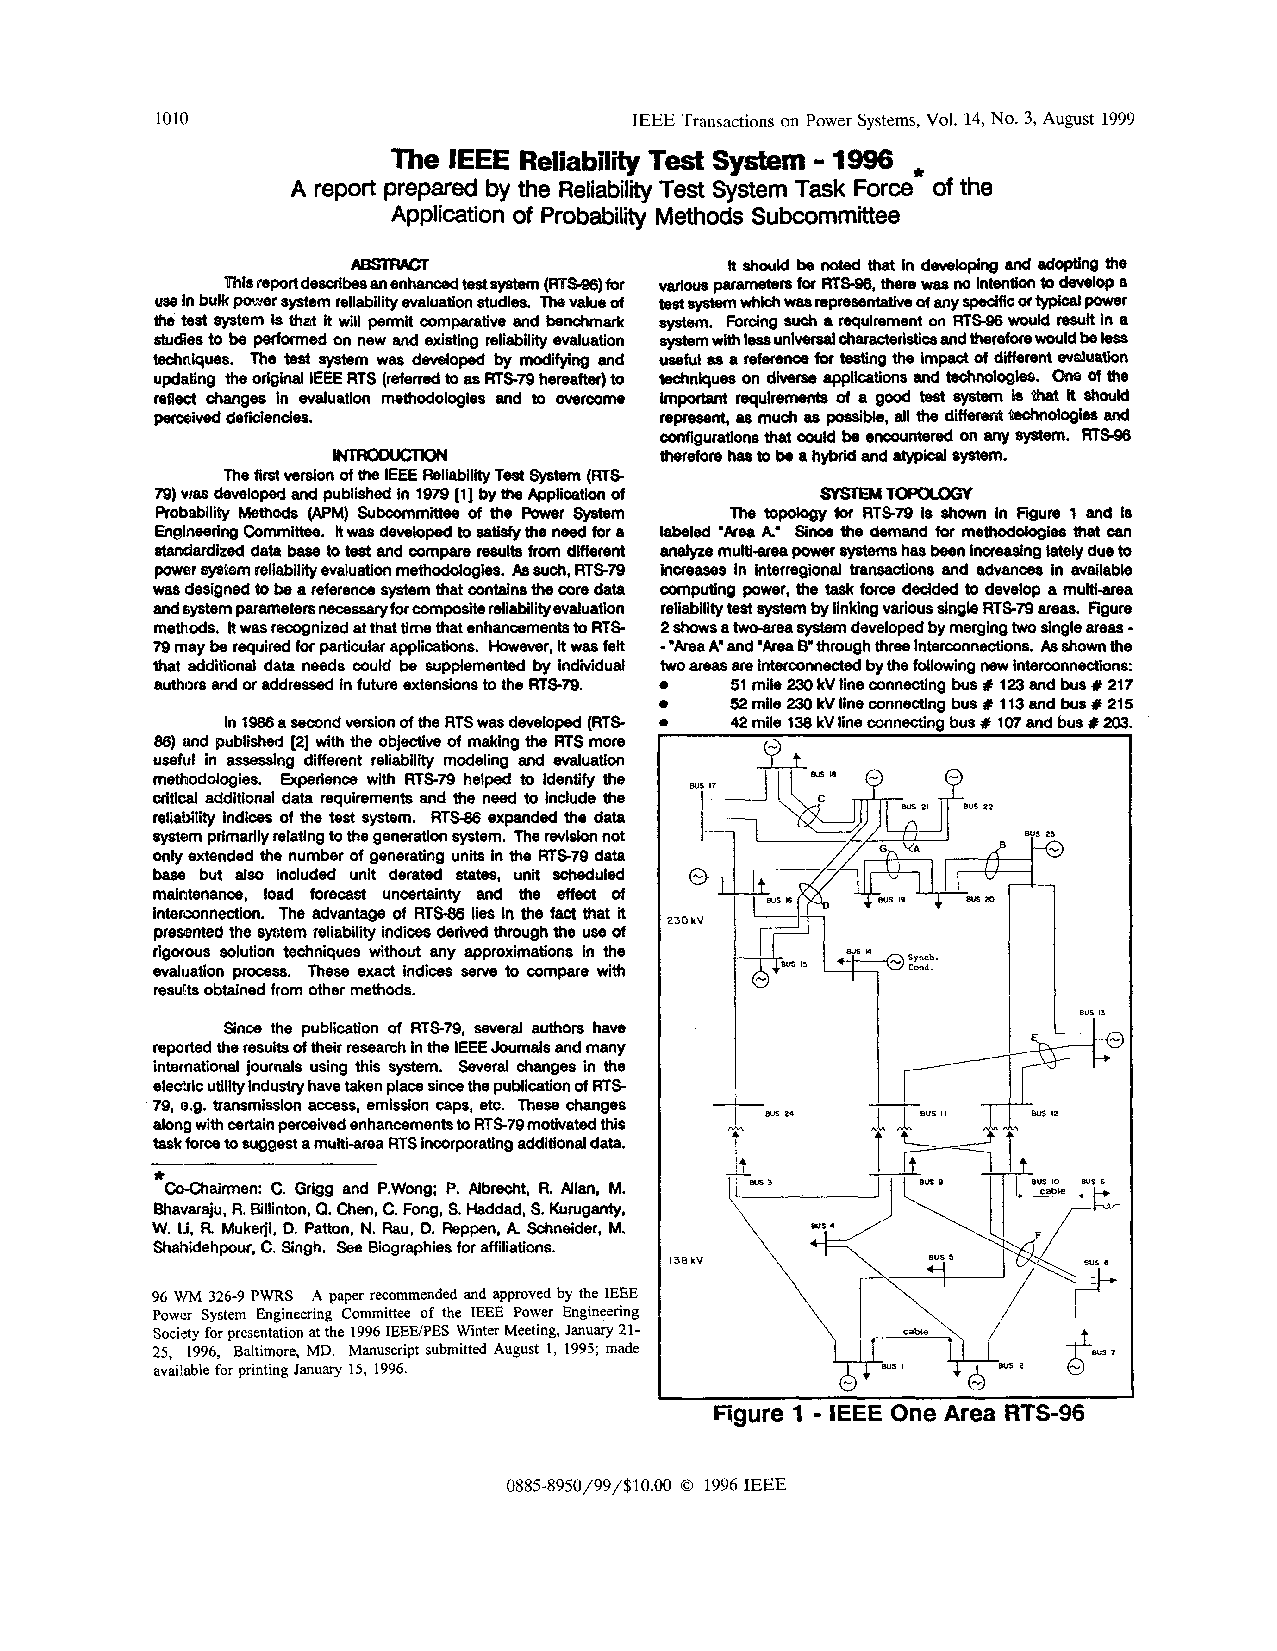
\includepdf[pages=1-last]{RTS96.pdf}


% ================================================================== %
\chapter{Published Papers}

\begin{large}
\begin{enumerate}
\item Comparing Security Assessment Schemes Through Two-Stage Monte Carlo Sampling
\item Analyzing Security Assessment Schemes in Traditional Networks
\item An Optimized Defence Plan for a Power System
\item Controlled Islanding Scheme for Power Systems
\item Analysis of the National 8th November 2003 Libyan Blackout
\item Design of a Transient Stability Scheme to Prevent Cascading Blackouts
\end{enumerate}
\end{large}

\pagebreak

% ------------------------------------------------------------------------------

\begin{center}\begin{large}
{\Huge Paper 1}
\vspace{40px}

Comparing Security Assessment Schemes Through Two-Stage Monte Carlo Sampling
\vspace{40px}

Brooks, J.; Dunn, R.;
\vspace{40px}

Universities Power Engineering Conference, 2010. UPEC 2010. 45th International
\end{large}\end{center}

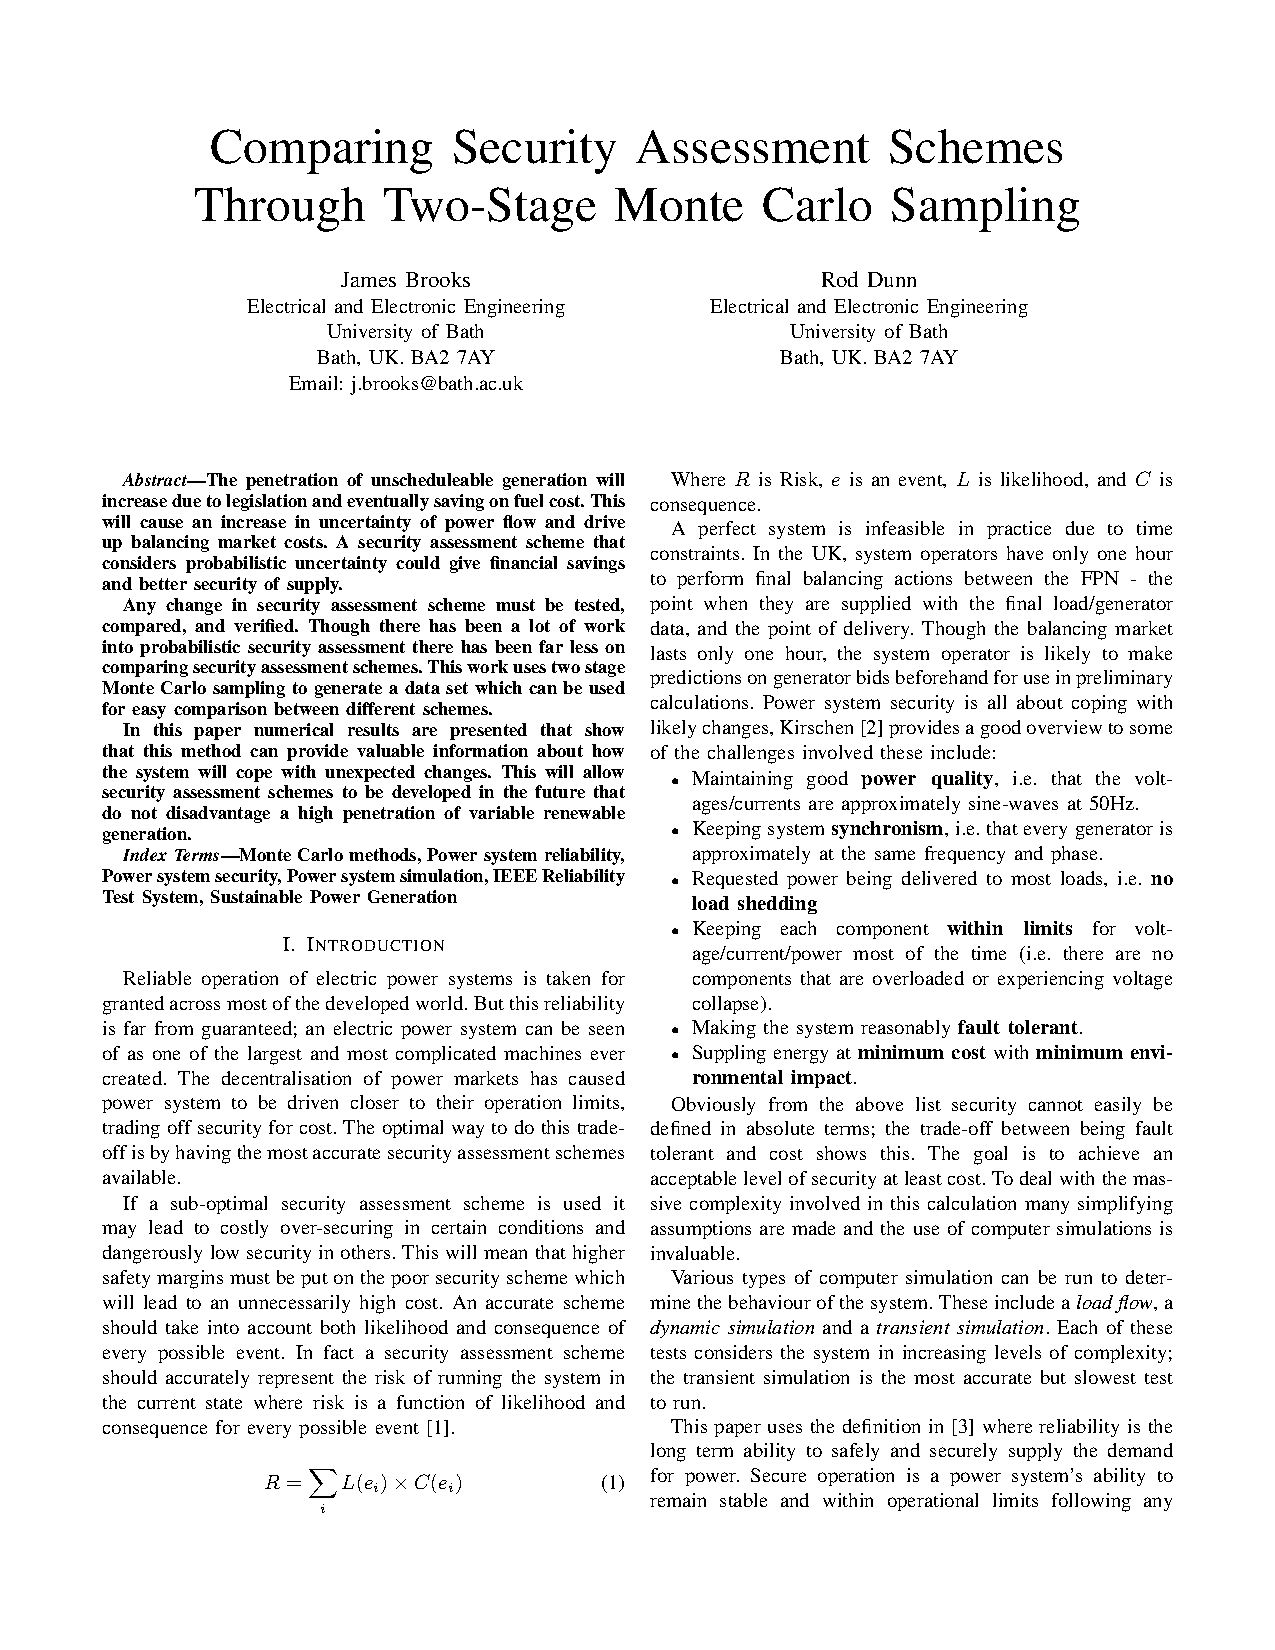
\includepdf[pages=1-last]{getPDF6.pdf}

% ------------------------------------------------------------------------------

\begin{center}\begin{large}
{\Huge Paper 2}
\vspace{40px}

Analyzing Security Assessment Schemes in Traditional Networks
\vspace{40px}

Brooks, J.; Dunn, R.;
\vspace{40px}

Sustainable Power Generation and Supply, 2009. SUPERGEN '09. International Conference on
\vspace{60px}

Digital Object Identifier: 10.1109/SUPERGEN.2009.5348262

Publication Year: 2009 , Page(s): 1 - 6
\end{large}\end{center}

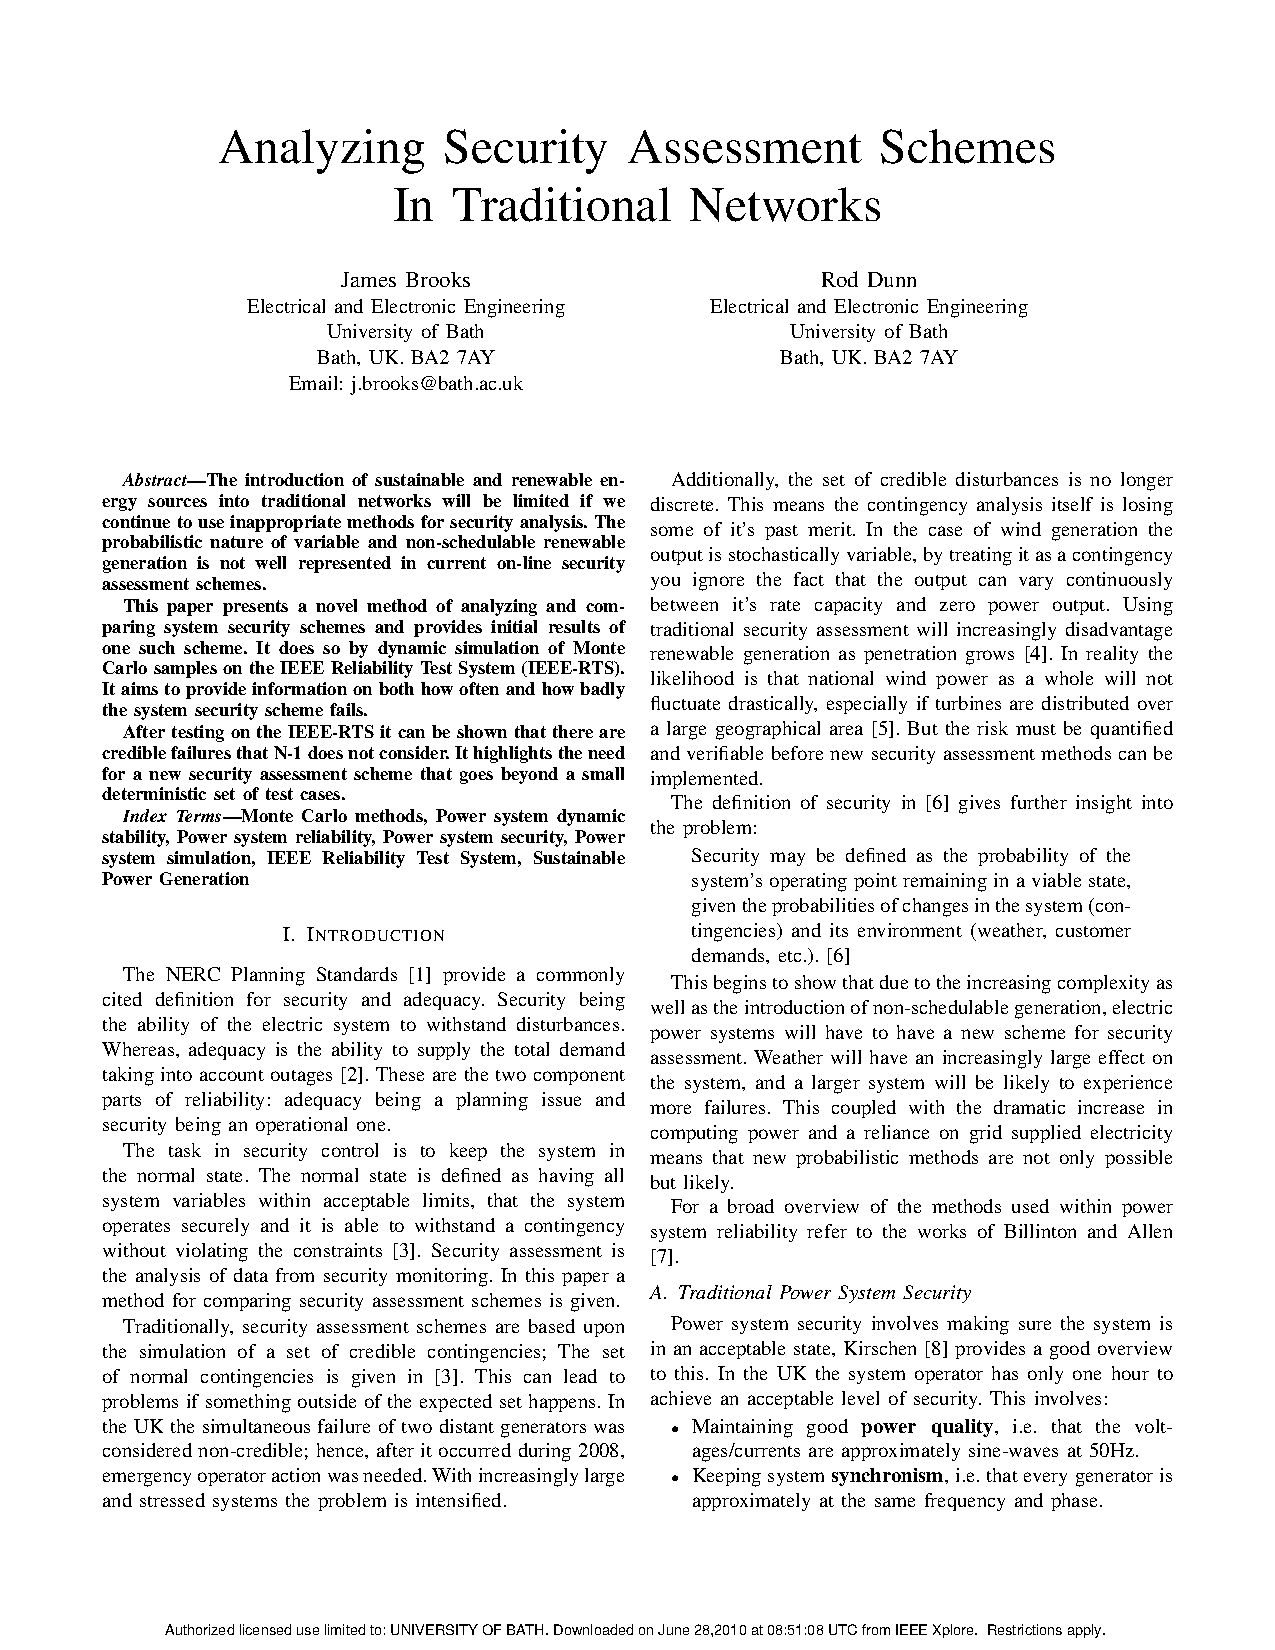
\includepdf[pages=1-last]{getPDF4.pdf}

% ------------------------------------------------------------------------------

\begin{center}\begin{large}
{\Huge Paper 3}
\vspace{40px}

An Optimized Defence Plan for a Power System
\vspace{40px}

El-Werfelli, M.; Brooks, J.; Dunn, R.;
\vspace{40px}

Universities Power Engineering Conference, 2008. UPEC 2008. 43rd International
\vspace{40px}

Digital Object Identifier: 10.1109/UPEC.2008.4651470

Publication Year: 2008 , Page(s): 1 - 6
\end{large}\end{center}

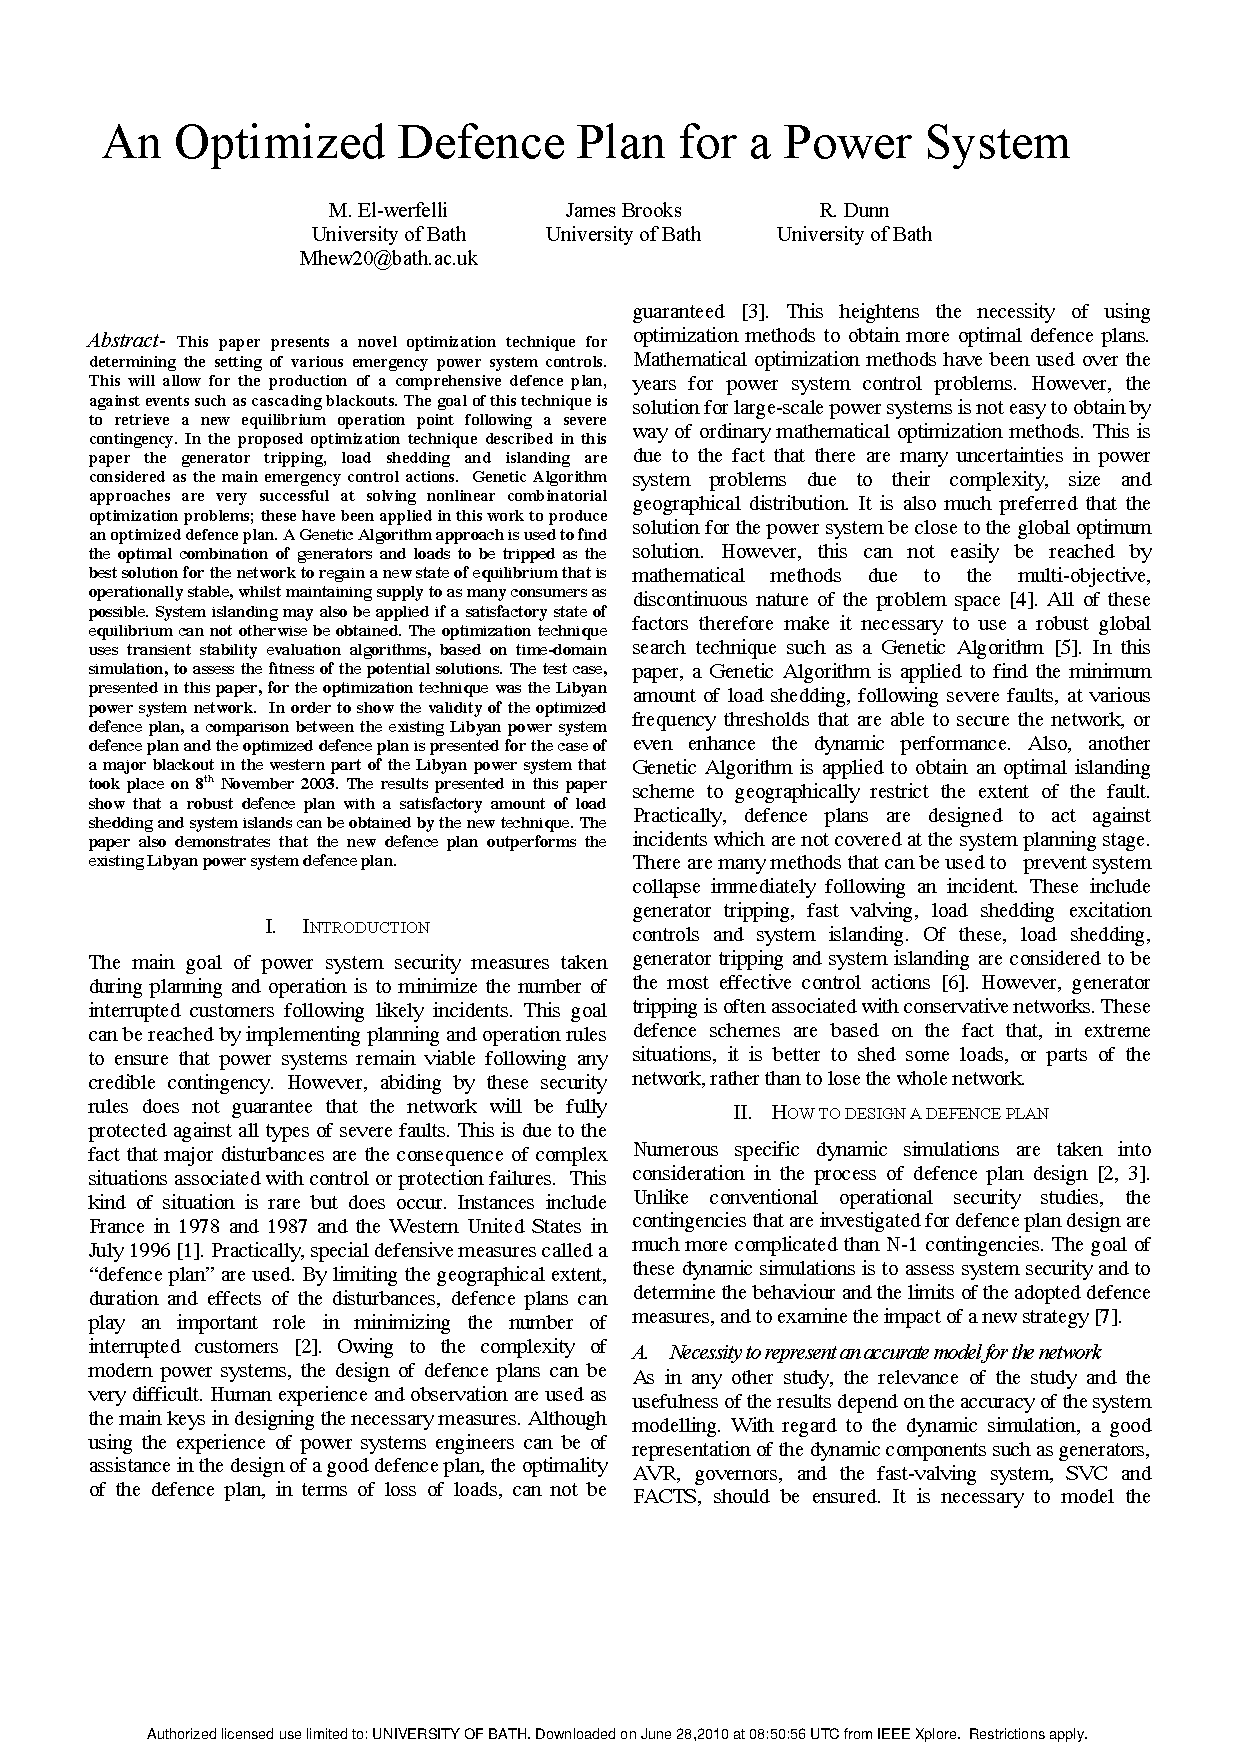
\includepdf[pages=1-last]{getPDF2.pdf}

% ------------------------------------------------------------------------------

\begin{center}\begin{large}
{\Huge Paper 4}
\vspace{40px}

Controlled Islanding Scheme for Power Systems
\vspace{40px}

El-Werfelli, M.; Brooks, J.; Dunn, R.;
\vspace{40px}

Universities Power Engineering Conference, 2008. UPEC 2008. 43rd International
\vspace{40px}

Digital Object Identifier: 10.1109/UPEC.2008.4651471

Publication Year: 2008 , Page(s): 1 - 6
\end{large}\end{center}

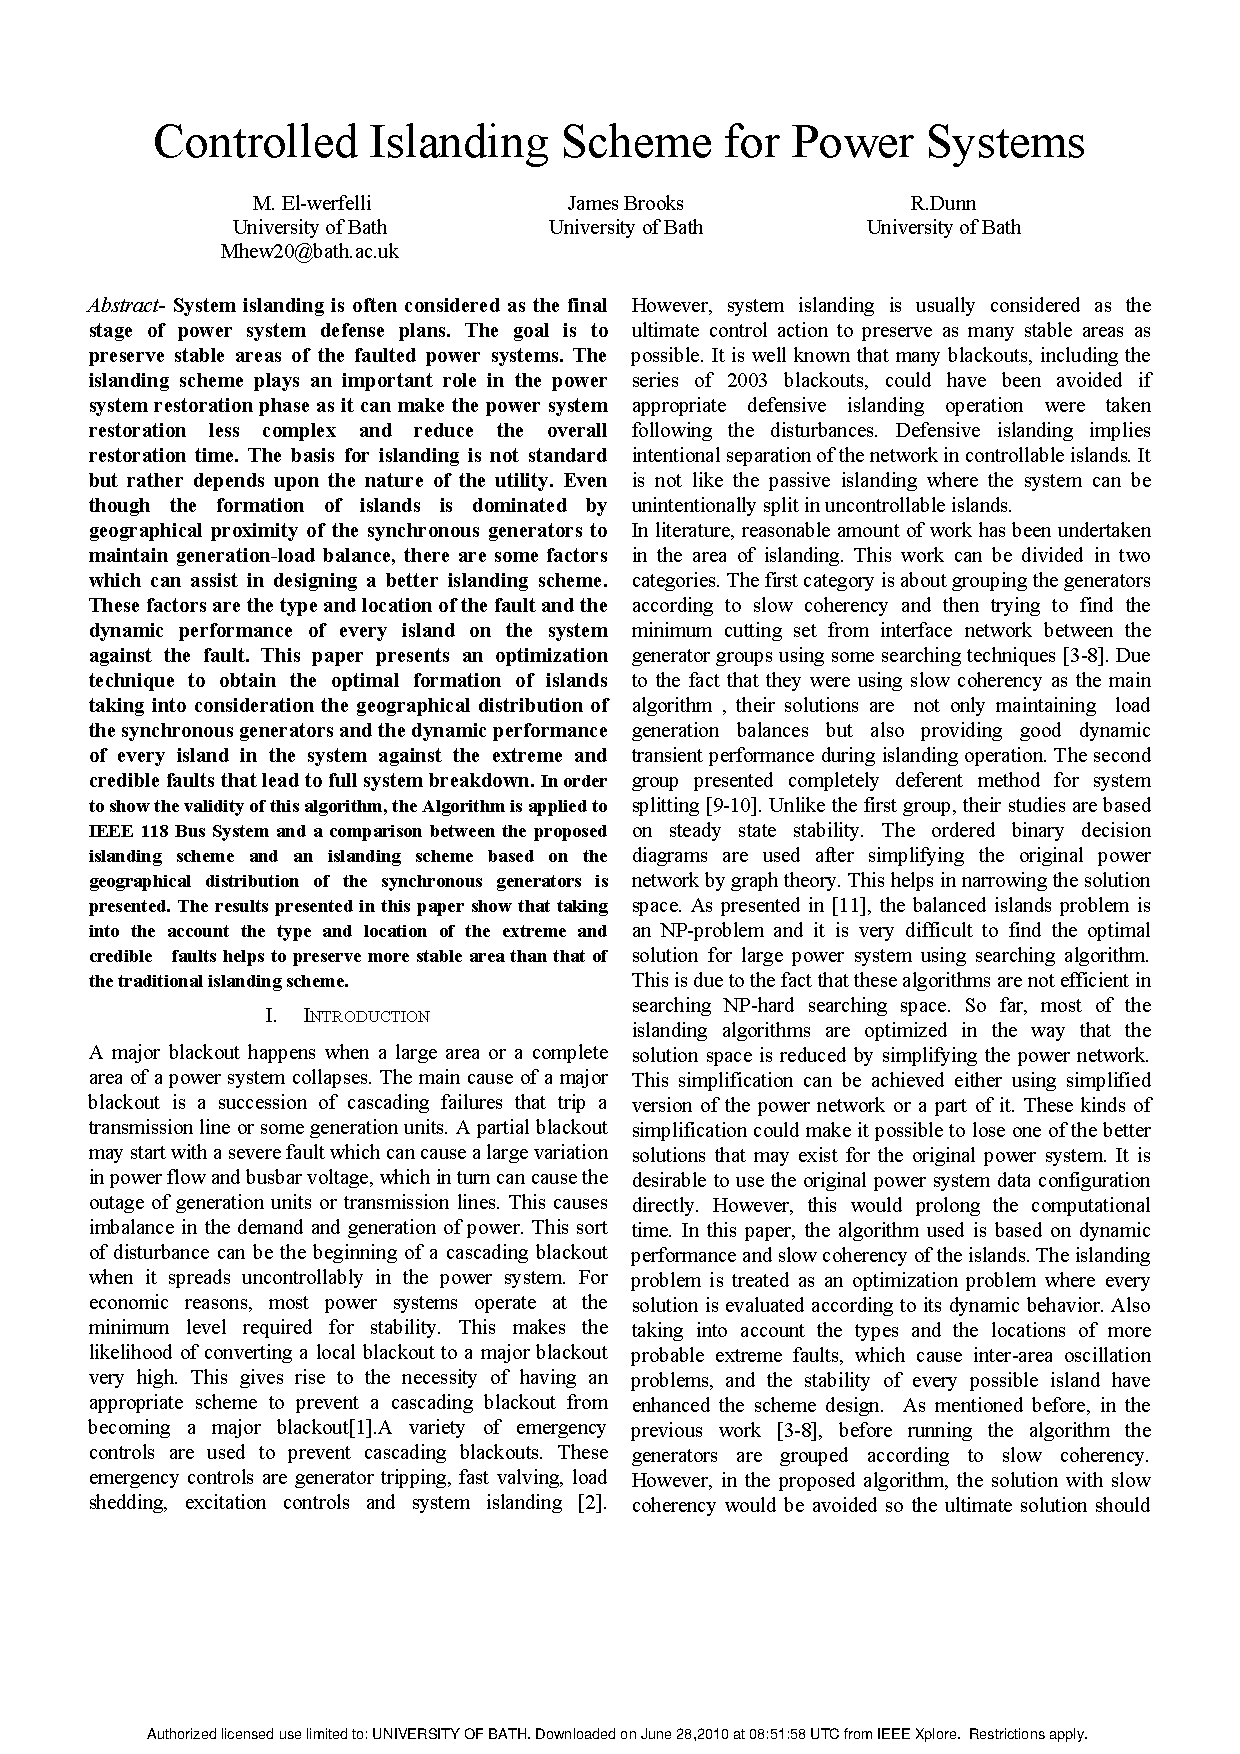
\includepdf[pages=1-last]{getPDF5.pdf}

% ------------------------------------------------------------------------------

\begin{center}\begin{large}
{\Huge Paper 5}
\vspace{40px}

Analysis of the National 8th November 2003 Libyan Blackout
\vspace{40px}

El-Werfelli, M.; Dunn, R.; Redfern, M.; Brooks, J.;
\vspace{40px}

Universities Power Engineering Conference, 2008. UPEC 2008. 43rd International
\vspace{40px}

Digital Object Identifier: 10.1109/UPEC.2008.4651469

Publication Year: 2008 , Page(s): 1 - 5
\end{large}\end{center}

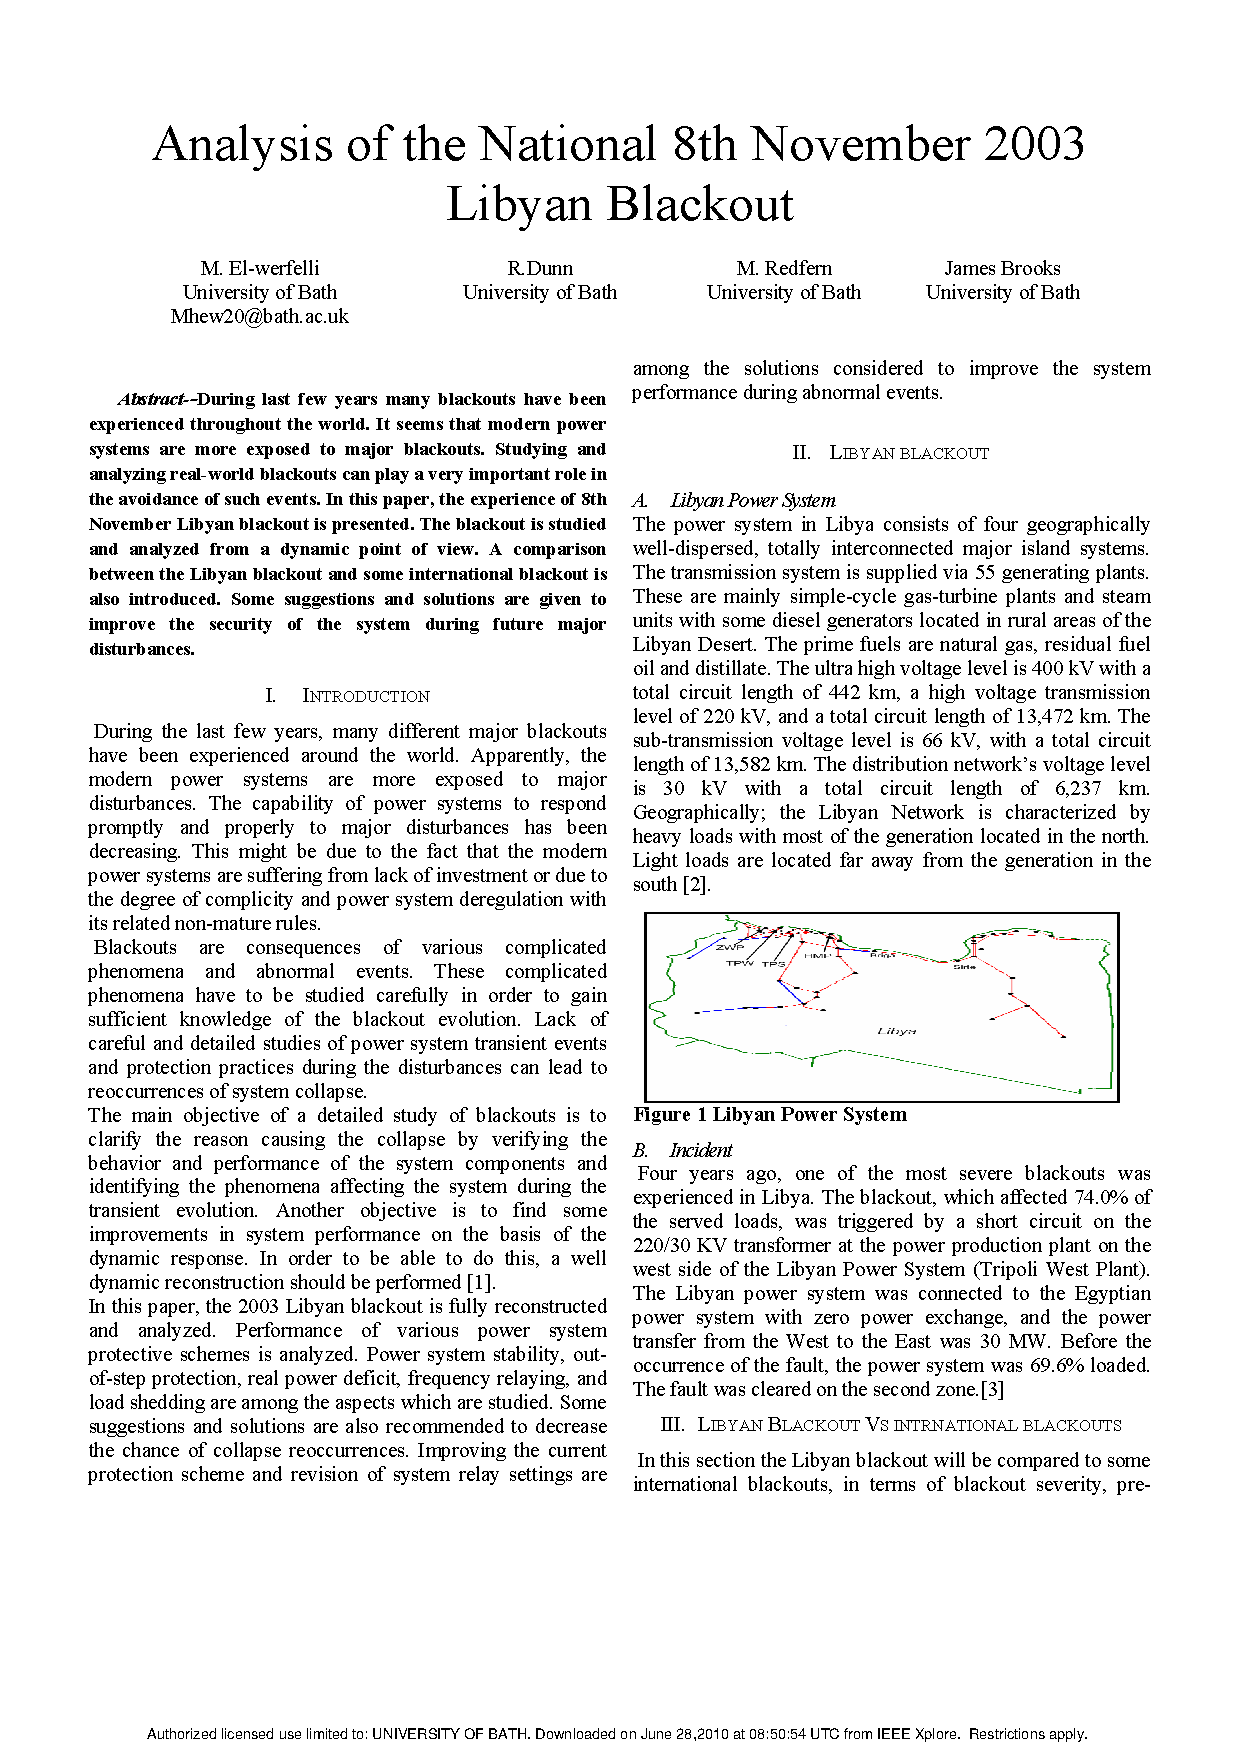
\includepdf[pages=1-last]{getPDF.pdf}

% ------------------------------------------------------------------------------

\begin{center}\begin{large}
{\Huge Paper 6}
\vspace{40px}

Design of a Transient Stability Scheme to Prevent Cascading Blackouts
\vspace{40px}

El-Werfelli, M.H.; Dunn, R.; Brooks, J.;
\vspace{40px}

Universities Power Engineering Conference, 2007. UPEC 2007. 42nd International
\vspace{40px}

Digital Object Identifier: 10.1109/UPEC.2007.4468987

Publication Year: 2007 , Page(s): 443 - 448
\end{large}\end{center}

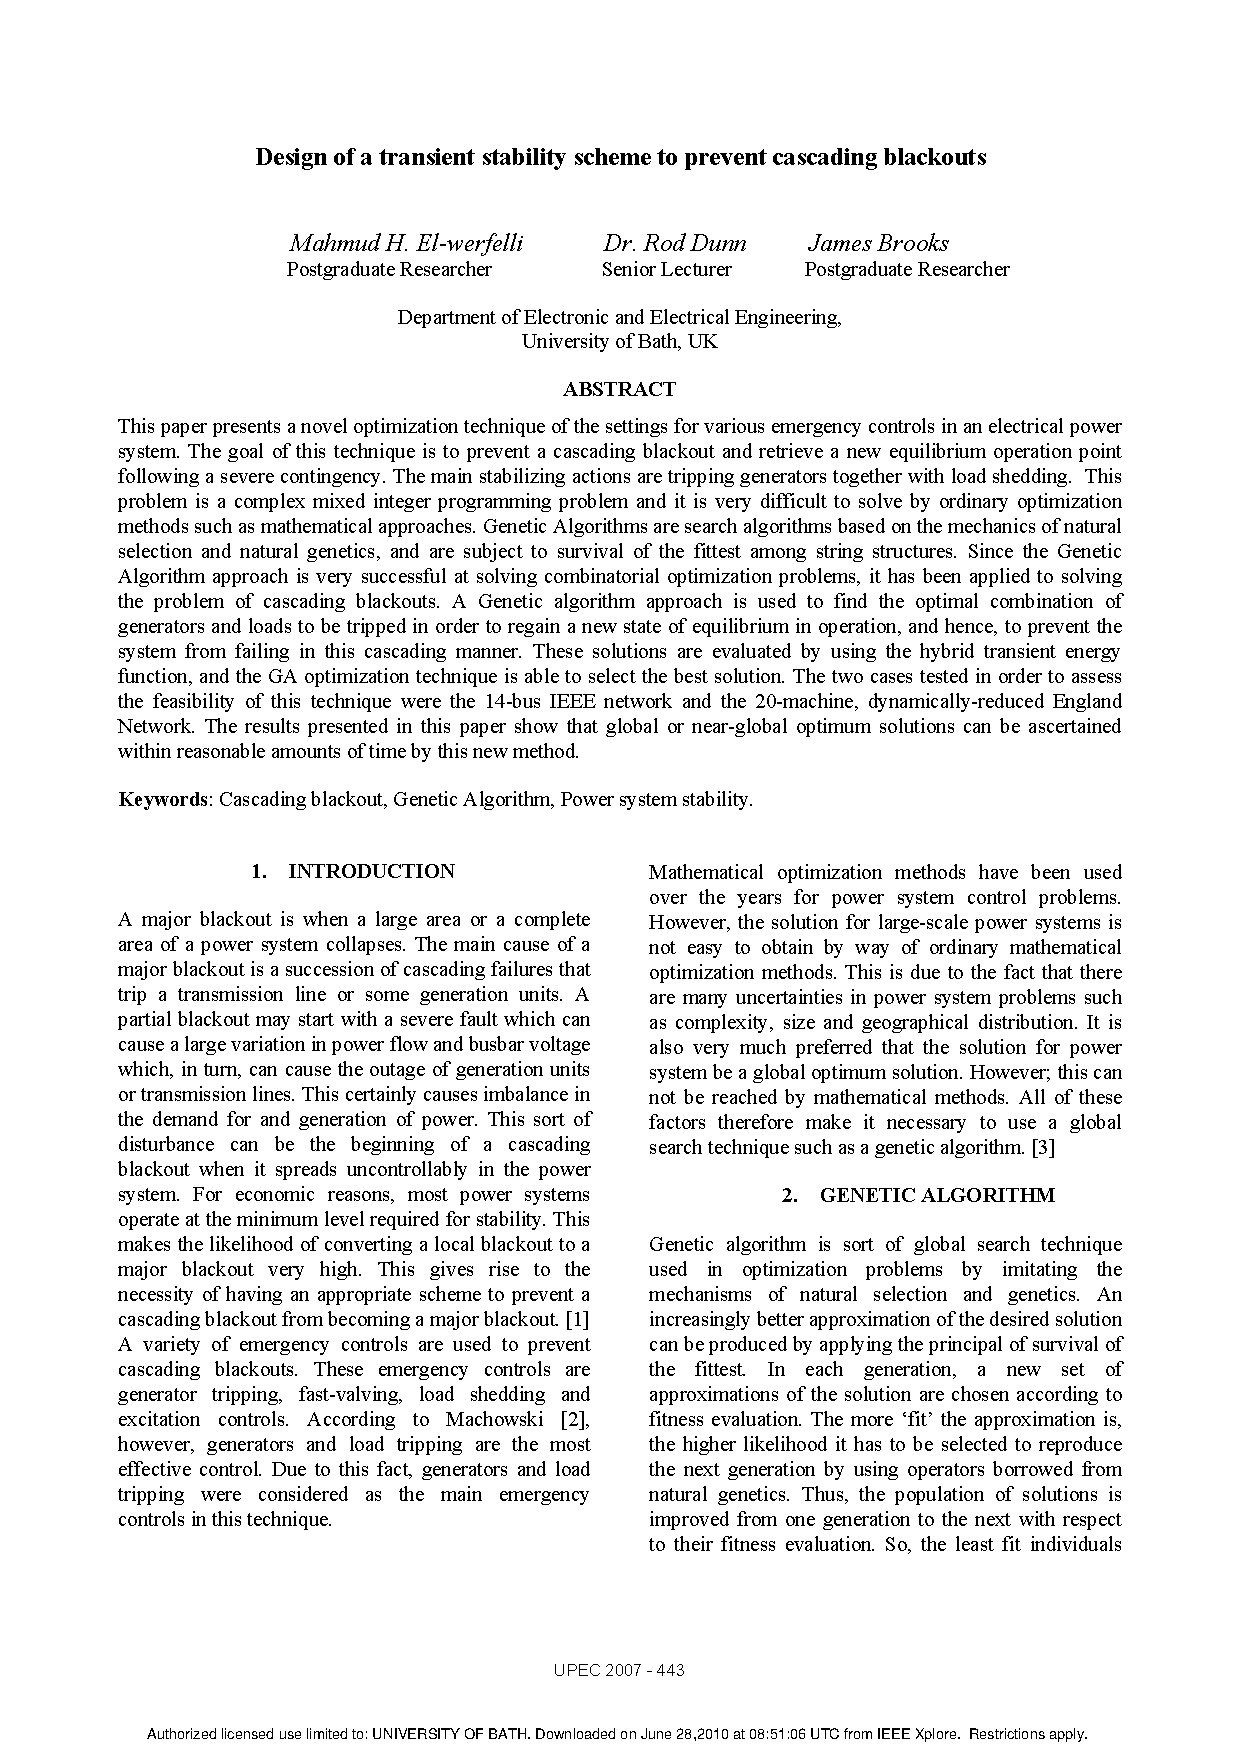
\includepdf[pages=1-last]{getPDF3.pdf}


% ================================================================== %
\chapter{Fix Power Mismatch Code}\label{lbl_sec_code}

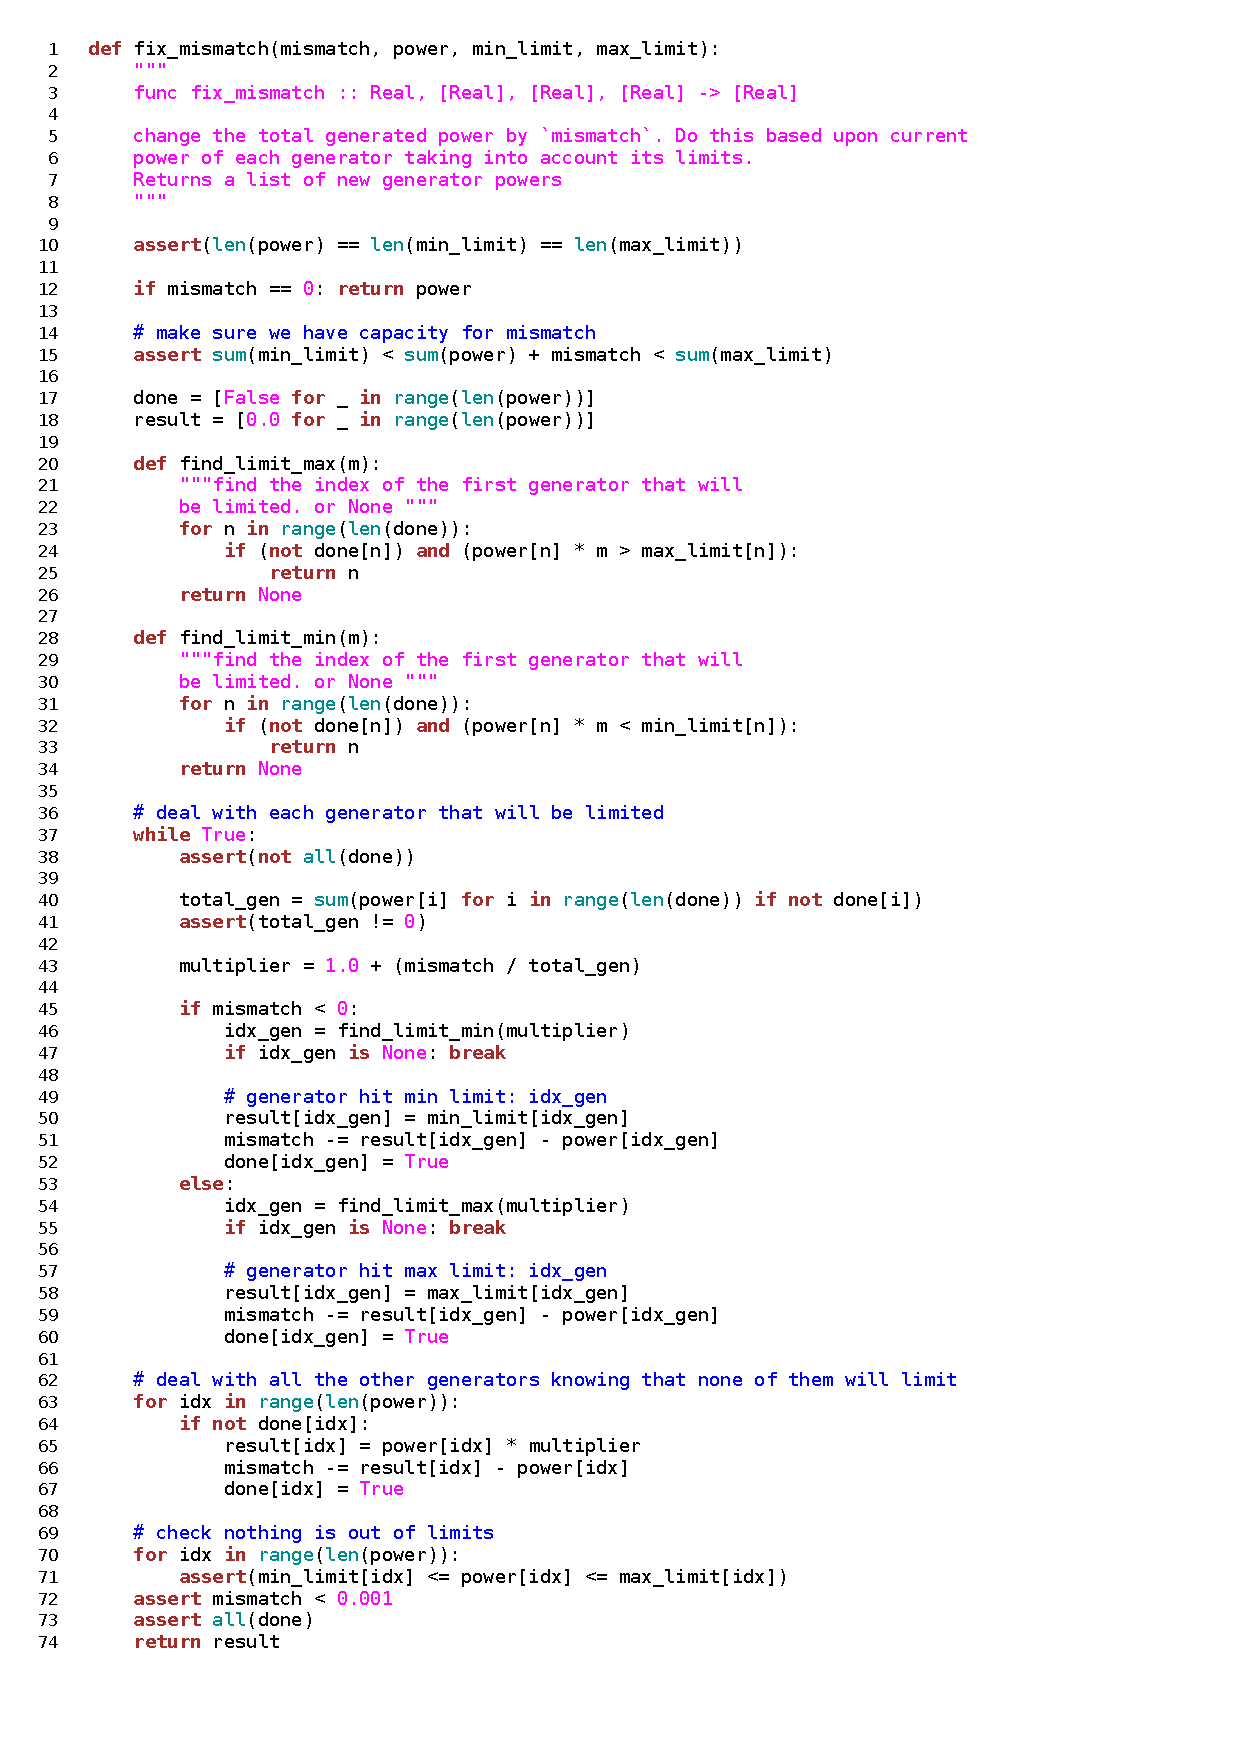
\includepdf[pages=1-last]{code.pdf}


% ================================================================== %
\backmatter
\addcontentsline{toc}{chapter}{Bibliography}
\bibliographystyle{abbrv}
\bibliography{all}
% ================================================================== %
\end{document}
% ================================================================== %

% LocalWords:  synchronism renewables unscheduleable islanded lineariziation
% LocalWords:  scheduleable parallelizable SAS memoization intermittency GA ANN
% LocalWords:  MTTF MCP NWP USD HistoricPowerUse historicpoweruse png quo GW Ph
% LocalWords:  rainforest installedcapacity photovoltaics Zhang MacKay Kundur
% LocalWords:  Jamasb Billinton Ackerman physicalstructure busbars TSO Transco
% LocalWords:  DSO economicstructure FPN ukmarket SBP SSP Elexon's weeklydemand
% LocalWords:  AVR SVC CHP CCGT ROC et al DSM NERC stabilityclassification XYZ
% LocalWords:  busbar BWEA DTI Ofgem PSS rotorsmallstability AVRs de SCIG Kling
% LocalWords:  rotorlargestability HistoricBladeSize windhubheight Slootweg th
% LocalWords:  DFIG Ackermann UK's Pelamis generationtypes Interruptable SCADA
% LocalWords:  everyone's PSAT electro ODEs EMPT simulatortimescales Dandeno RK
% LocalWords:  Arrillaga Brenan HVDC Matlab PSSENG Wheatley Ascher Milano Eqn
% LocalWords:  localerror globalerror Heun's Runge Kutta Multi Lengyel multi PV
% LocalWords:  Moulton CSR CSC SIMD pipelining GPU GPGPU FPGA SCOPF PQ OPF SO's
% LocalWords:  WindPowerCurve windpowercurve Polinder Palsson TSOs Kirschen Img
% LocalWords:  perfectSAS perfectsas Sobajic McCalley Xiao stochastically PRNG
% LocalWords:  Pudaruth Mersenne MTTR memoized pdf Werfelli Redfern UPEC getPDF
% LocalWords:  nd IEEE RTS MCS SO SQSS facto
